% ======= NỘI DUNG =======
\chapter{Phân tích và Thiết kế}
\label{chap:PhanTichVaThietKe}

\section{Phân tích}
\label{sec:PhanTich}

% ======= NỘI DUNG PHẦN PHÂN TÍCH USE CASE =======
\subsection{Mô hình hóa tương tác (Use-case Diagram)}
\label{subsec:BieuDoCaSuDung}

Phần phân tích use case được xây dựng theo phạm vi hệ thống đã hiện thực. Hệ
thống có các tác nhân chính gồm \textbf{Khách}, \textbf{Bạn đọc},
\textbf{Thủ thư} và \textbf{Quản trị viên}; ngoài ra còn có các hệ thống phụ
trợ như \textbf{Google OAuth}, \textbf{PayOS}, \textbf{Dịch vụ Email} và
\textbf{Gemini API}. Để tránh một sơ đồ quá dày, use case được trình bày thành
một sơ đồ tổng quát và sáu sơ đồ module chi tiết.

\begin{figure}[H]
 \centering
 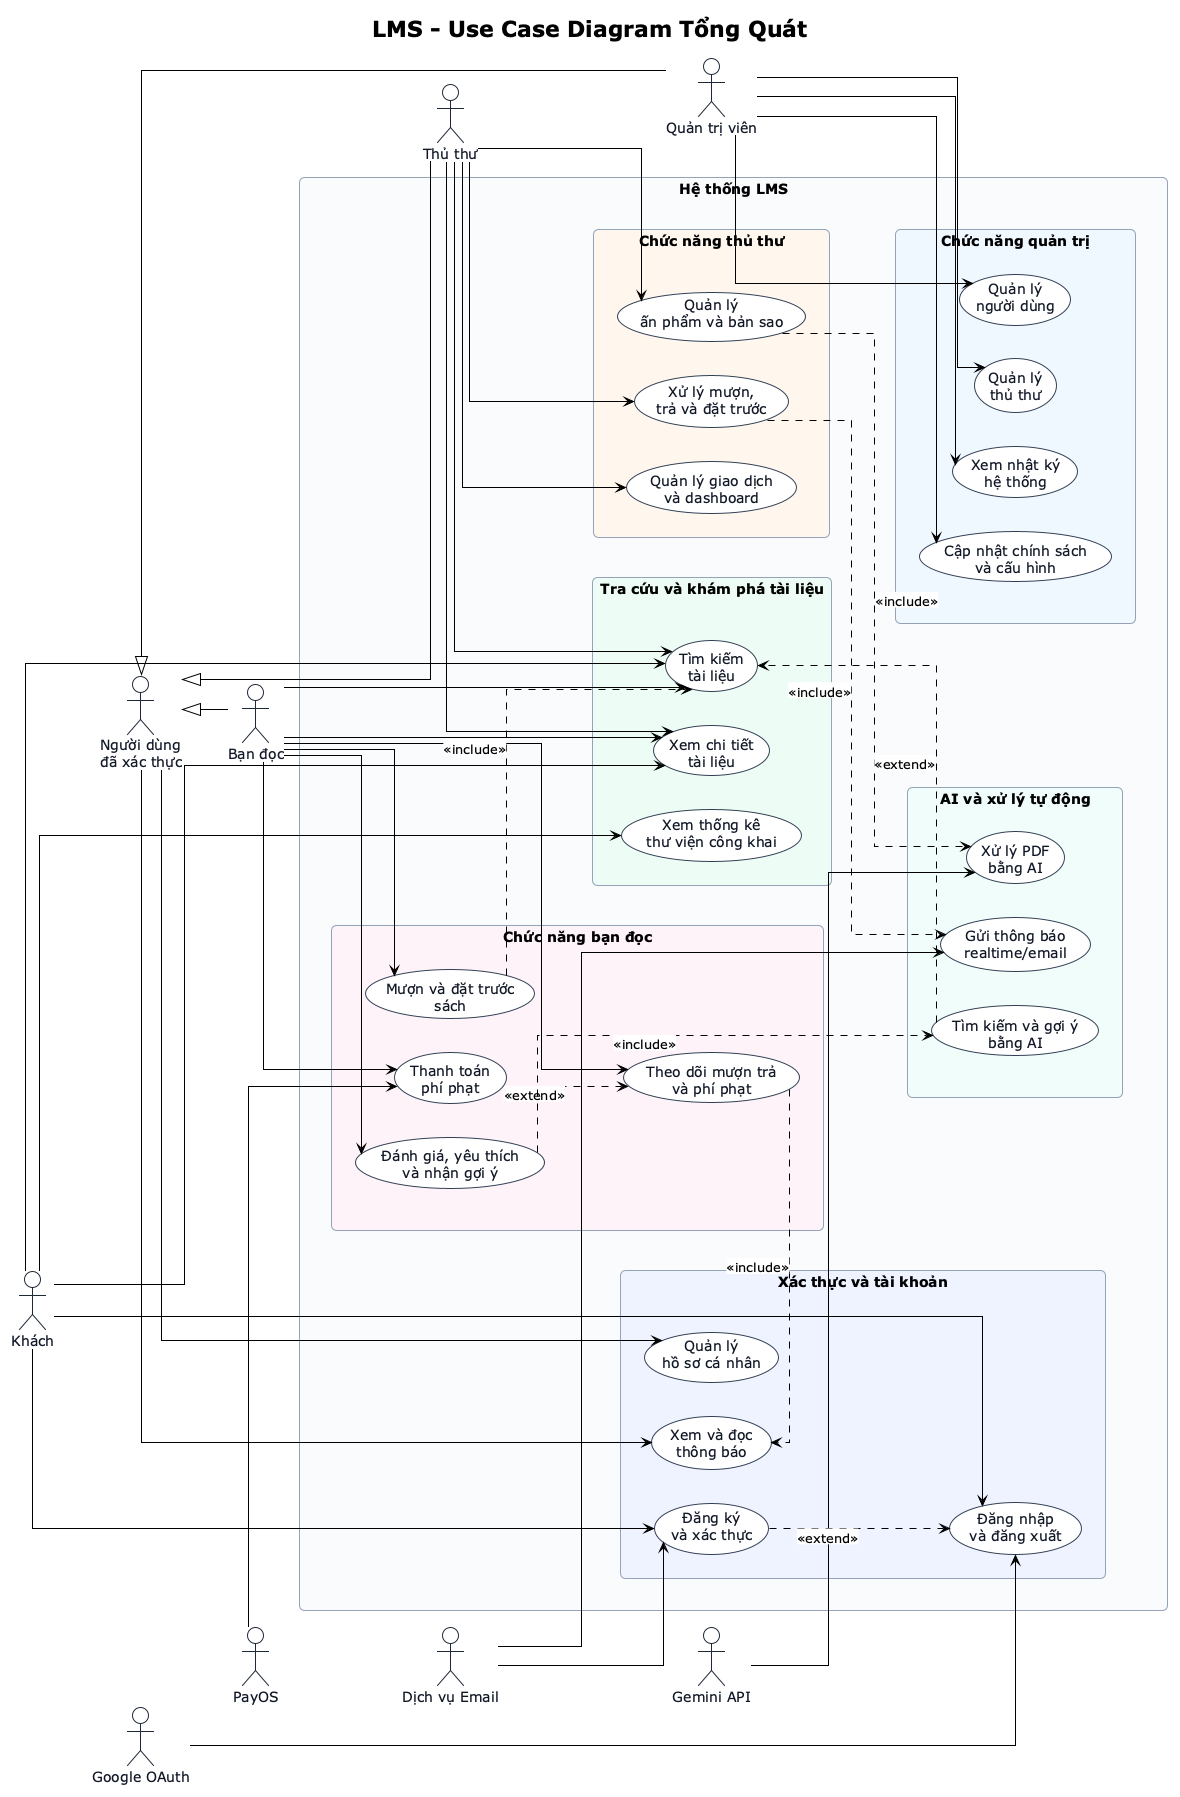
\includegraphics[width=\linewidth, height=0.82\textheight, keepaspectratio]{figures/ch05/usecase/overview.png}
 \caption{Biểu đồ Use Case tổng quát}
 \label{fig:usecase_overview}
\end{figure}

\begin{figure}[H]
 \centering
 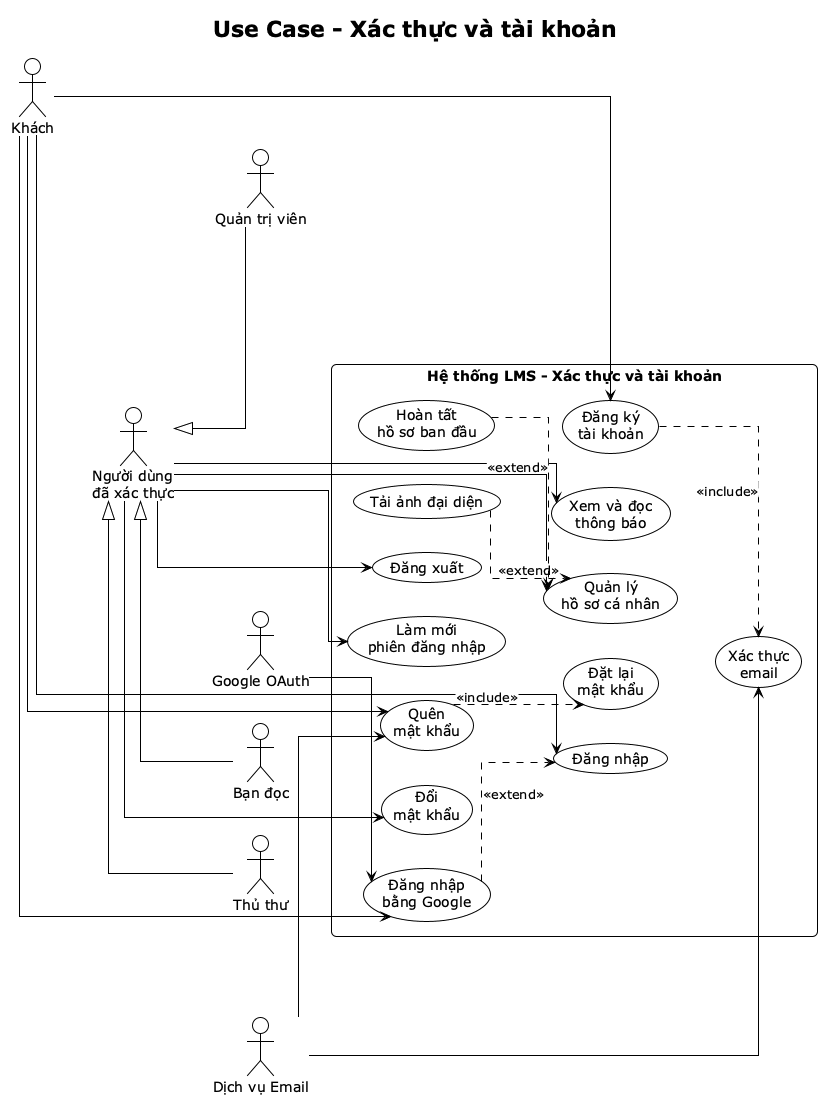
\includegraphics[width=\linewidth, height=0.78\textheight, keepaspectratio]{figures/ch05/usecase/modules/01_auth_account.png}
 \caption{Use Case module Xác thực và tài khoản}
 \label{fig:usecase_auth_account}
\end{figure}

\begin{figure}[H]
 \centering
 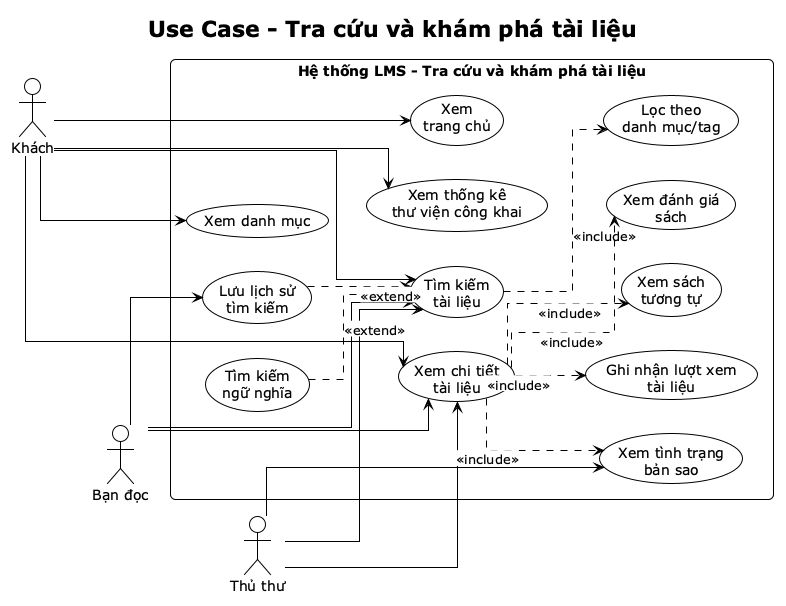
\includegraphics[width=\linewidth, height=0.78\textheight, keepaspectratio]{figures/ch05/usecase/modules/02_discovery_catalog.png}
 \caption{Use Case module Tra cứu và khám phá tài liệu}
 \label{fig:usecase_discovery_catalog}
\end{figure}

\begin{figure}[H]
 \centering
 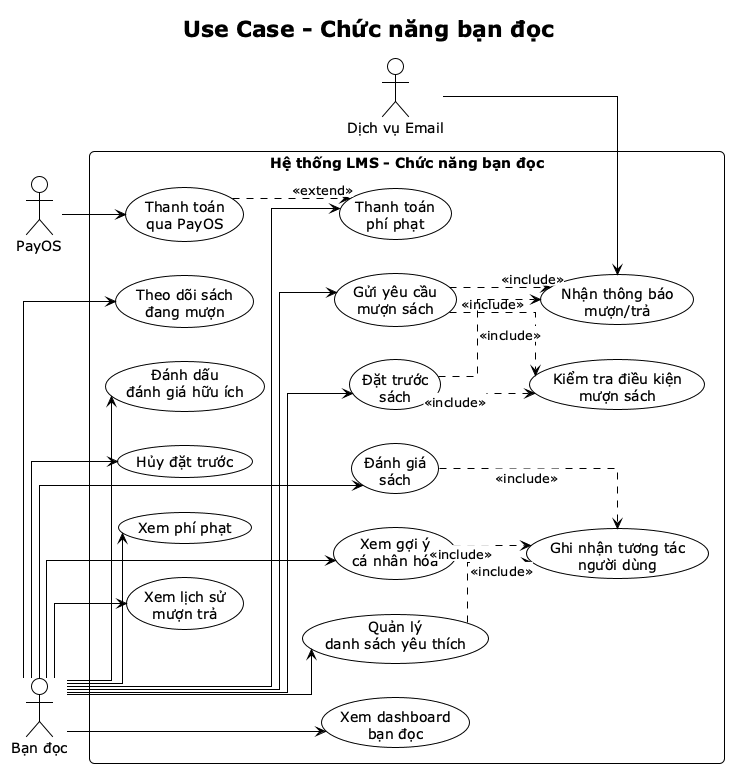
\includegraphics[width=\linewidth, height=0.78\textheight, keepaspectratio]{figures/ch05/usecase/modules/03_reader_services.png}
 \caption{Use Case module Chức năng bạn đọc}
 \label{fig:usecase_reader_services}
\end{figure}

\begin{figure}[H]
 \centering
 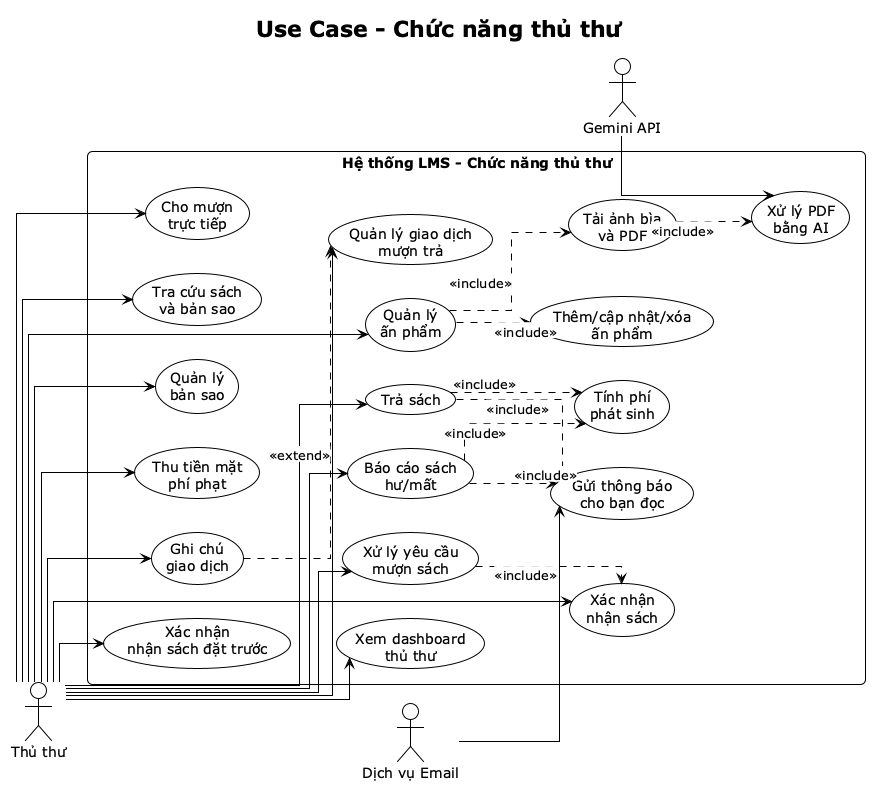
\includegraphics[width=\linewidth, height=0.78\textheight, keepaspectratio]{figures/ch05/usecase/modules/04_librarian_operations.png}
 \caption{Use Case module Chức năng thủ thư}
 \label{fig:usecase_librarian_operations}
\end{figure}

\begin{figure}[H]
 \centering
 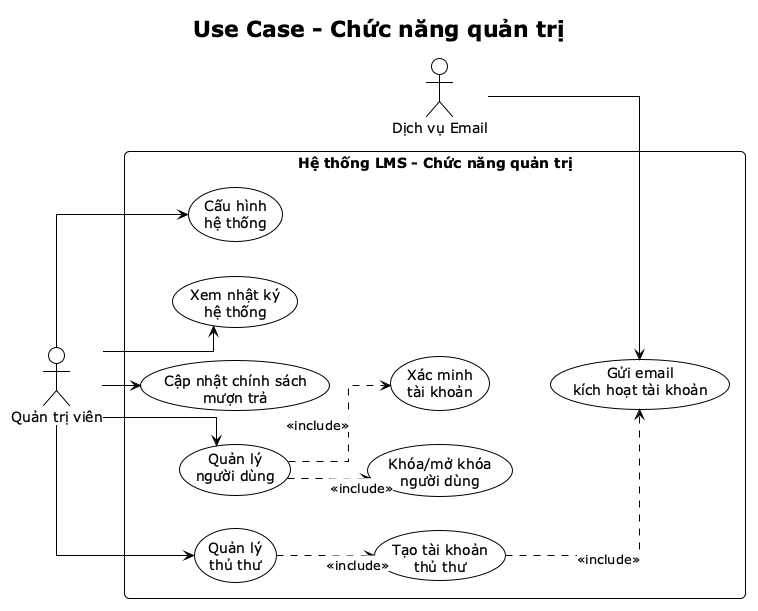
\includegraphics[width=\linewidth, height=0.78\textheight, keepaspectratio]{figures/ch05/usecase/modules/05_admin_management.png}
 \caption{Use Case module Chức năng quản trị}
 \label{fig:usecase_admin_management}
\end{figure}

\begin{figure}[H]
 \centering
 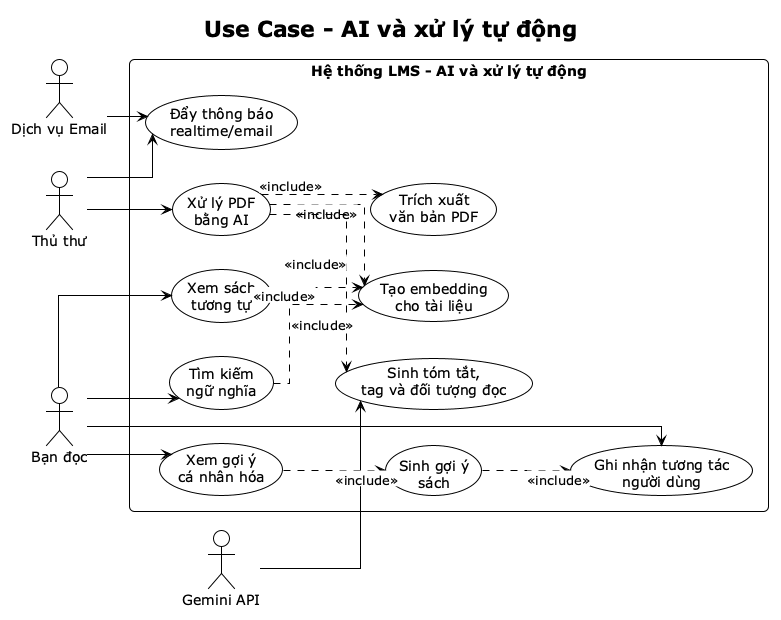
\includegraphics[width=\linewidth, height=0.78\textheight, keepaspectratio]{figures/ch05/usecase/modules/06_ai_automation.png}
 \caption{Use Case module AI và xử lý tự động}
 \label{fig:usecase_ai_automation}
\end{figure}

Sơ đồ tổng quát trong Hình~\ref{fig:usecase_overview} cho thấy ranh giới chính
của hệ thống: nhóm xác thực/tài khoản, nhóm tra cứu tài liệu, nhóm nghiệp vụ
bạn đọc, nhóm nghiệp vụ thủ thư, nhóm quản trị và nhóm AI tự động. Các sơ đồ
module từ Hình~\ref{fig:usecase_auth_account} đến
Hình~\ref{fig:usecase_ai_automation} làm rõ các quan hệ
\texttt{include}/\texttt{extend}: đăng ký bao gồm xác thực email; tìm kiếm có
thể mở rộng sang semantic search; mượn/đặt trước bao gồm kiểm tra điều kiện
mượn; upload PDF bao gồm xử lý AI; trả sách và báo hư/mất bao gồm tính phí và
gửi thông báo.

\begin{table}[H]
\centering
\caption{Đối chiếu nhóm Use Case với hiện thực hệ thống}
\label{tab:usecase_mapping_reality}
\begin{tabularx}{\linewidth}{|p{0.22\linewidth}|>{\raggedright\arraybackslash}X|>{\raggedright\arraybackslash}X|}
\hline
\textbf{Nhóm} & \textbf{Use case chính} & \textbf{Hiện thực tương ứng} \\
\hline
Xác thực và tài khoản & Đăng ký, xác thực email, đăng nhập thường, đăng nhập Google, refresh token, quên/đặt lại mật khẩu, hồ sơ, avatar, đổi mật khẩu, thông báo & Auth/User modules, OAuth2 Google, JWT/refresh token, email verification/reset password, profile API và notification API. \\
\hline
Tra cứu và khám phá tài liệu & Trang chủ, tìm kiếm catalog, semantic search, lọc danh mục/tag, chi tiết tài liệu, bản sao, đánh giá, sách tương tự, thống kê công khai & Public pages và catalog/recommendation API: \texttt{/api/v1/publications/search}, \texttt{/api/v1/ai/semantic-search}, \texttt{/api/v1/publications/\{id\}}, \texttt{/items}, \texttt{/ratings}, \texttt{/similar}. \\
\hline
Chức năng bạn đọc & Mượn, đặt trước, hủy đặt trước, theo dõi sách đang mượn, lịch sử mượn trả, phí phạt, PayOS, wishlist, rating, gợi ý cá nhân hóa & Reader pages, circulation/reservation/fine APIs, PayOS payment, wishlist/rating APIs và recommendation API. \\
\hline
Chức năng thủ thư & Quản lý ấn phẩm, bản sao, upload bìa/PDF, AI ETL, xử lý yêu cầu mượn, mượn trực tiếp, trả sách, báo hư/mất, ghi chú giao dịch, thu tiền mặt & Librarian pages, catalog/item APIs, presigned upload, backend AI gateway, circulation transaction APIs, fine cash payment và notification/email events. \\
\hline
Chức năng quản trị & Quản lý thủ thư, quản lý người dùng, khóa/mở khóa, xác minh tài khoản, chính sách mượn trả, nhật ký hệ thống & Admin pages và admin APIs: librarian/user management, circulation policy, audit log và account verification. \\
\hline
AI và xử lý tự động & Semantic search, recommendation, sách tương tự, xử lý PDF, trích xuất text, embedding, sinh summary/tag/audience, ghi nhận tương tác, realtime/email notification & AI service FastAPI/Celery, RabbitMQ, Gemini API, PostgreSQL pgvector, interaction tracking, Kafka/email/WebSocket notification. \\
\hline
\end{tabularx}
\end{table}

\subsubsection{Đặc tả các nhóm Use Case chính}
\begin{table}[H]
\centering
\caption{Bảng đặc tả UC-01: Xác thực và tài khoản}
\label{tab:uc_auth_account}
\begin{tabularx}{\linewidth}{|p{0.24\linewidth}|>{\raggedright\arraybackslash}X|}
\hline
\textbf{Thuộc tính} & \textbf{Mô tả chi tiết} \\
\hline
\textbf{Tên Use Case} & Xác thực và tài khoản \\
\hline
\textbf{Mã số} & UC-01 \\
\hline
\textbf{Tác nhân} & Khách, Người dùng đã xác thực, Bạn đọc, Thủ thư, Quản trị viên, Google OAuth, Dịch vụ Email \\
\hline
\textbf{Mô tả ngắn gọn} & Quản lý vòng đời đăng ký, xác thực email, đăng nhập thường/Google, refresh token, quên mật khẩu, đặt lại mật khẩu, hồ sơ cá nhân, avatar, đổi mật khẩu và thông báo người dùng. \\
\hline
\textbf{Tiền điều kiện} & Người dùng truy cập trang đăng ký/đăng nhập hoặc đã có phiên đăng nhập hợp lệ khi thao tác với hồ sơ và thông báo. \\
\hline
\textbf{Hậu điều kiện} & \textbf{Thành công:} Tài khoản được tạo/xác thực, phiên đăng nhập được cấp, thông tin hồ sơ hoặc trạng thái thông báo được cập nhật. \newline \textbf{Thất bại:} Hệ thống giữ nguyên dữ liệu và trả thông báo lỗi xác thực, validation hoặc quyền truy cập. \\
\hline
\textbf{Luồng chính} &
1. Khách đăng ký tài khoản hoặc đăng nhập bằng email/mật khẩu hoặc Google OAuth. \newline
2. Backend kiểm tra dữ liệu, mã hóa mật khẩu, tạo token hoặc xử lý callback OAuth2. \newline
3. Với tài khoản mới hoặc quên mật khẩu, hệ thống gửi email xác thực/đặt lại mật khẩu. \newline
4. Người dùng đã xác thực quản lý hồ sơ, avatar, mật khẩu và đọc thông báo. \newline
5. Hệ thống cập nhật trạng thái tài khoản, refresh token, hồ sơ hoặc notification tương ứng. \\
\hline
\textbf{Luồng thay thế} &
\textbf{Email đã tồn tại hoặc token hết hạn:} hệ thống trả lỗi và yêu cầu người dùng nhập lại hoặc gửi lại email. \newline
\textbf{OAuth2 không hợp lệ:} backend từ chối callback và chuyển người dùng về luồng đăng nhập. \\
\hline
\end{tabularx}
\end{table}

\begin{table}[H]
\centering
\caption{Bảng đặc tả UC-02: Tra cứu và khám phá tài liệu}
\label{tab:uc_discovery_catalog}
\begin{tabularx}{\linewidth}{|p{0.24\linewidth}|>{\raggedright\arraybackslash}X|}
\hline
\textbf{Thuộc tính} & \textbf{Mô tả chi tiết} \\
\hline
\textbf{Tên Use Case} & Tra cứu và khám phá tài liệu \\
\hline
\textbf{Mã số} & UC-02 \\
\hline
\textbf{Tác nhân} & Khách, Bạn đọc, Thủ thư \\
\hline
\textbf{Mô tả ngắn gọn} & Cho phép người dùng xem trang chủ, tìm kiếm catalog, tìm kiếm ngữ nghĩa, lọc theo danh mục/tag, xem chi tiết tài liệu, bản sao, đánh giá, sách tương tự và thống kê công khai. \\
\hline
\textbf{Tiền điều kiện} & Catalog có dữ liệu ấn phẩm; với semantic search, tài liệu liên quan đã có vector embedding trong AI database. \\
\hline
\textbf{Hậu điều kiện} & \textbf{Thành công:} Danh sách hoặc chi tiết ấn phẩm được hiển thị, lịch sử tìm kiếm/lượt xem được ghi nhận khi phù hợp. \newline \textbf{Thất bại:} Hệ thống hiển thị trạng thái không có kết quả hoặc thông báo lỗi dịch vụ AI. \\
\hline
\textbf{Luồng chính} &
1. Người dùng nhập từ khóa, chọn bộ lọc hoặc nhập truy vấn tự nhiên. \newline
2. Frontend gọi API catalog search hoặc semantic search. \newline
3. Backend lọc catalog bằng PostgreSQL hoặc chuyển truy vấn sang AI service để tìm vector gần nhất. \newline
4. Hệ thống trả danh sách ấn phẩm, trạng thái bản sao, rating, AI summary và sách tương tự. \newline
5. Khi người dùng mở chi tiết, hệ thống ghi nhận lượt xem và hiển thị metadata liên quan. \\
\hline
\textbf{Luồng thay thế} &
\textbf{Không có kết quả:} giao diện hiển thị trạng thái rỗng và giữ bộ lọc để người dùng điều chỉnh. \newline
\textbf{AI service không sẵn sàng:} hệ thống vẫn có thể dùng tìm kiếm catalog thông thường. \\
\hline
\end{tabularx}
\end{table}

\begin{table}[H]
\centering
\caption{Bảng đặc tả UC-03: Chức năng bạn đọc}
\label{tab:uc_reader_services}
\begin{tabularx}{\linewidth}{|p{0.24\linewidth}|>{\raggedright\arraybackslash}X|}
\hline
\textbf{Thuộc tính} & \textbf{Mô tả chi tiết} \\
\hline
\textbf{Tên Use Case} & Chức năng bạn đọc \\
\hline
\textbf{Mã số} & UC-03 \\
\hline
\textbf{Tác nhân} & Bạn đọc, PayOS, Dịch vụ Email \\
\hline
\textbf{Mô tả ngắn gọn} & Cho phép bạn đọc xem dashboard, gửi yêu cầu mượn, đặt trước, hủy đặt trước, theo dõi sách đang mượn, xem lịch sử, xem/thanh toán phí phạt, quản lý wishlist, đánh giá sách và nhận gợi ý cá nhân hóa. \\
\hline
\textbf{Tiền điều kiện} & Bạn đọc đã đăng nhập, tài khoản hoạt động và không vi phạm các điều kiện nghiệp vụ đang được kiểm tra như giới hạn mượn hoặc phí phạt chưa thanh toán. \\
\hline
\textbf{Hậu điều kiện} & \textbf{Thành công:} Giao dịch mượn/đặt trước/phí phạt/wishlist/rating được cập nhật; tương tác người dùng được ghi nhận cho recommendation. \newline \textbf{Thất bại:} Hệ thống giữ nguyên trạng thái và trả thông báo lỗi. \\
\hline
\textbf{Luồng chính} &
1. Bạn đọc xem dashboard và mở chi tiết tài liệu. \newline
2. Bạn đọc gửi yêu cầu mượn hoặc đặt trước; backend kiểm tra chính sách mượn và trạng thái bản sao. \newline
3. Hệ thống tạo giao dịch hoặc reservation, gửi thông báo/email khi cần. \newline
4. Bạn đọc theo dõi sách đang mượn, lịch sử, phí phạt và thanh toán qua PayOS nếu chọn thanh toán online. \newline
5. Bạn đọc thêm wishlist, đánh giá sách hoặc xem gợi ý cá nhân hóa; hệ thống ghi nhận tương tác. \\
\hline
\textbf{Luồng thay thế} &
\textbf{Không đủ điều kiện mượn:} hệ thống từ chối yêu cầu và nêu lý do. \newline
\textbf{Thanh toán PayOS thất bại:} phí phạt giữ trạng thái chưa thanh toán để xử lý lại hoặc thu tiền mặt. \\
\hline
\end{tabularx}
\end{table}

\begin{table}[H]
\centering
\caption{Bảng đặc tả UC-04: Chức năng thủ thư}
\label{tab:uc_librarian_operations}
\begin{tabularx}{\linewidth}{|p{0.24\linewidth}|>{\raggedright\arraybackslash}X|}
\hline
\textbf{Thuộc tính} & \textbf{Mô tả chi tiết} \\
\hline
\textbf{Tên Use Case} & Chức năng thủ thư \\
\hline
\textbf{Mã số} & UC-04 \\
\hline
\textbf{Tác nhân} & Thủ thư, Dịch vụ Email, Gemini API \\
\hline
\textbf{Mô tả ngắn gọn} & Thủ thư quản lý ấn phẩm, bản sao, file bìa/PDF, kích hoạt AI ETL, xử lý mượn/trả/đặt trước, báo hư/mất, ghi chú giao dịch, thu tiền mặt và gửi thông báo cho bạn đọc. \\
\hline
\textbf{Tiền điều kiện} & Thủ thư đã đăng nhập và có quyền thao tác với catalog/circulation. Các barcode, publication hoặc transaction liên quan tồn tại trong hệ thống. \\
\hline
\textbf{Hậu điều kiện} & \textbf{Thành công:} Catalog, bản sao, giao dịch, phí phạt hoặc trạng thái AI ETL được cập nhật; thông báo/email được gửi khi nghiệp vụ yêu cầu. \newline \textbf{Thất bại:} Dữ liệu không đổi và hệ thống hiển thị lỗi. \\
\hline
\textbf{Luồng chính} &
1. Thủ thư quản lý metadata ấn phẩm, bản sao và upload file bìa/PDF. \newline
2. Khi upload PDF, backend lưu URL tài liệu và kích hoạt AI ETL để xử lý nội dung. \newline
3. Thủ thư tra cứu bạn đọc, barcode, yêu cầu mượn hoặc reservation. \newline
4. Hệ thống xử lý mượn trực tiếp, xác nhận nhận sách, trả sách, báo hư/mất và tính phí phát sinh. \newline
5. Thủ thư theo dõi dashboard/giao dịch, ghi chú nghiệp vụ và thu tiền mặt khi cần. \\
\hline
\textbf{Luồng thay thế} &
\textbf{Barcode/giao dịch không hợp lệ:} hệ thống từ chối cập nhật. \newline
\textbf{AI service lỗi:} trạng thái ETL ghi nhận thất bại, catalog vẫn lưu metadata thủ công để thủ thư xử lý lại sau. \\
\hline
\end{tabularx}
\end{table}

\begin{table}[H]
\centering
\caption{Bảng đặc tả UC-05: Chức năng quản trị}
\label{tab:dt_admin_management}
\begin{tabularx}{\linewidth}{|p{0.24\linewidth}|>{\raggedright\arraybackslash}X|}
\hline
\textbf{Thuộc tính} & \textbf{Mô tả chi tiết} \\
\hline
\textbf{Tên Use Case} & Chức năng quản trị \\
\hline
\textbf{Mã số} & UC-05 \\
\hline
\textbf{Tác nhân} & Quản trị viên, Dịch vụ Email \\
\hline
\textbf{Mô tả ngắn gọn} & Quản trị viên quản lý tài khoản thủ thư, người dùng, trạng thái khóa/mở khóa, xác minh tài khoản, chính sách mượn trả, nhật ký hệ thống và cấu hình hệ thống. \\
\hline
\textbf{Tiền điều kiện} & Quản trị viên đã đăng nhập với vai trò admin. \\
\hline
\textbf{Hậu điều kiện} & Tài khoản, chính sách hoặc dữ liệu audit/config được cập nhật theo thao tác hợp lệ; email kích hoạt được gửi khi tạo tài khoản thủ thư. \\
\hline
\textbf{Luồng chính} & 1. Admin mở màn hình quản trị. \newline
2. Admin tạo/cập nhật tài khoản thủ thư hoặc quản lý người dùng. \newline
3. Hệ thống kiểm tra quyền, cập nhật trạng thái người dùng, gửi email kích hoạt nếu cần. \newline
4. Admin cập nhật chính sách mượn trả hoặc xem nhật ký hệ thống để kiểm soát vận hành. \\
\hline
\textbf{Luồng thay thế} & Nếu dữ liệu không hợp lệ hoặc admin không đủ quyền cho thao tác cụ thể, hệ thống từ chối và ghi nhận lỗi phù hợp. \\
\hline
\end{tabularx}
\end{table}

\begin{table}[H]
\centering
\caption{Bảng đặc tả UC-06: AI và xử lý tự động}
\label{tab:dt_ai_automation}
\begin{tabularx}{\linewidth}{|p{0.24\linewidth}|>{\raggedright\arraybackslash}X|}
\hline
\textbf{Thuộc tính} & \textbf{Mô tả chi tiết} \\
\hline
\textbf{Tên Use Case} & AI và xử lý tự động \\
\hline
\textbf{Mã số} & UC-06 \\
\hline
\textbf{Tác nhân} & Bạn đọc, Thủ thư, Gemini API, Dịch vụ Email \\
\hline
\textbf{Mô tả ngắn gọn} & AI service hỗ trợ semantic search, sách tương tự, recommendation, xử lý PDF, trích xuất text, tạo embedding, sinh summary/tag/audience, ghi nhận tương tác và đẩy thông báo realtime/email. \\
\hline
\textbf{Tiền điều kiện} & Tài liệu đã được upload hoặc người dùng có truy vấn/tương tác cần xử lý. AI service có thể truy cập database, RabbitMQ, model embedding và Gemini API khi cần sinh metadata. \\
\hline
\textbf{Hậu điều kiện} & Vector, metadata AI, recommendation cache hoặc notification được cập nhật. Nếu Gemini không khả dụng, pipeline ghi lỗi hoặc dùng fallback theo logic ETL. \\
\hline
\textbf{Luồng chính} & 1. Backend gửi yêu cầu xử lý tài liệu hoặc truy vấn AI. \newline
2. AI API nhận request, Celery worker xử lý job qua RabbitMQ. \newline
3. Worker trích xuất PDF, tạo embedding, ghi vector, gọi Gemini để sinh summary/tag/audience. \newline
4. Kết quả được ghi về PostgreSQL/pgvector và callback trạng thái về backend. \newline
5. Semantic search/recommendation dùng dữ liệu vector và tương tác người dùng để trả kết quả. \\
\hline
\textbf{Luồng thay thế} & Nếu LLM lỗi/quota, hệ thống ghi trạng thái thất bại hoặc dùng deterministic fallback; nếu chưa có vector, semantic search bỏ qua tài liệu đó cho đến khi ETL hoàn tất. \\
\hline
\end{tabularx}
\end{table}

\subsection{Mô hình lớp (Class diagram)}
\label{subsec:ClassDiagram}

Class diagram trong Hình~\ref{fig:class_diagram_lms} mô tả các lớp domain
chính của hệ thống theo nhóm User/Authentication, Catalog, Circulation,
Recommendation/AI và Payment/Notification. Sơ đồ tập trung vào entity, thuộc
tính nghiệp vụ, phương thức domain và quan hệ giữa các lớp, giúp liên kết phần
phân tích use case với thiết kế dữ liệu và cấu trúc backend.

\begin{figure}[H]
 \centering
 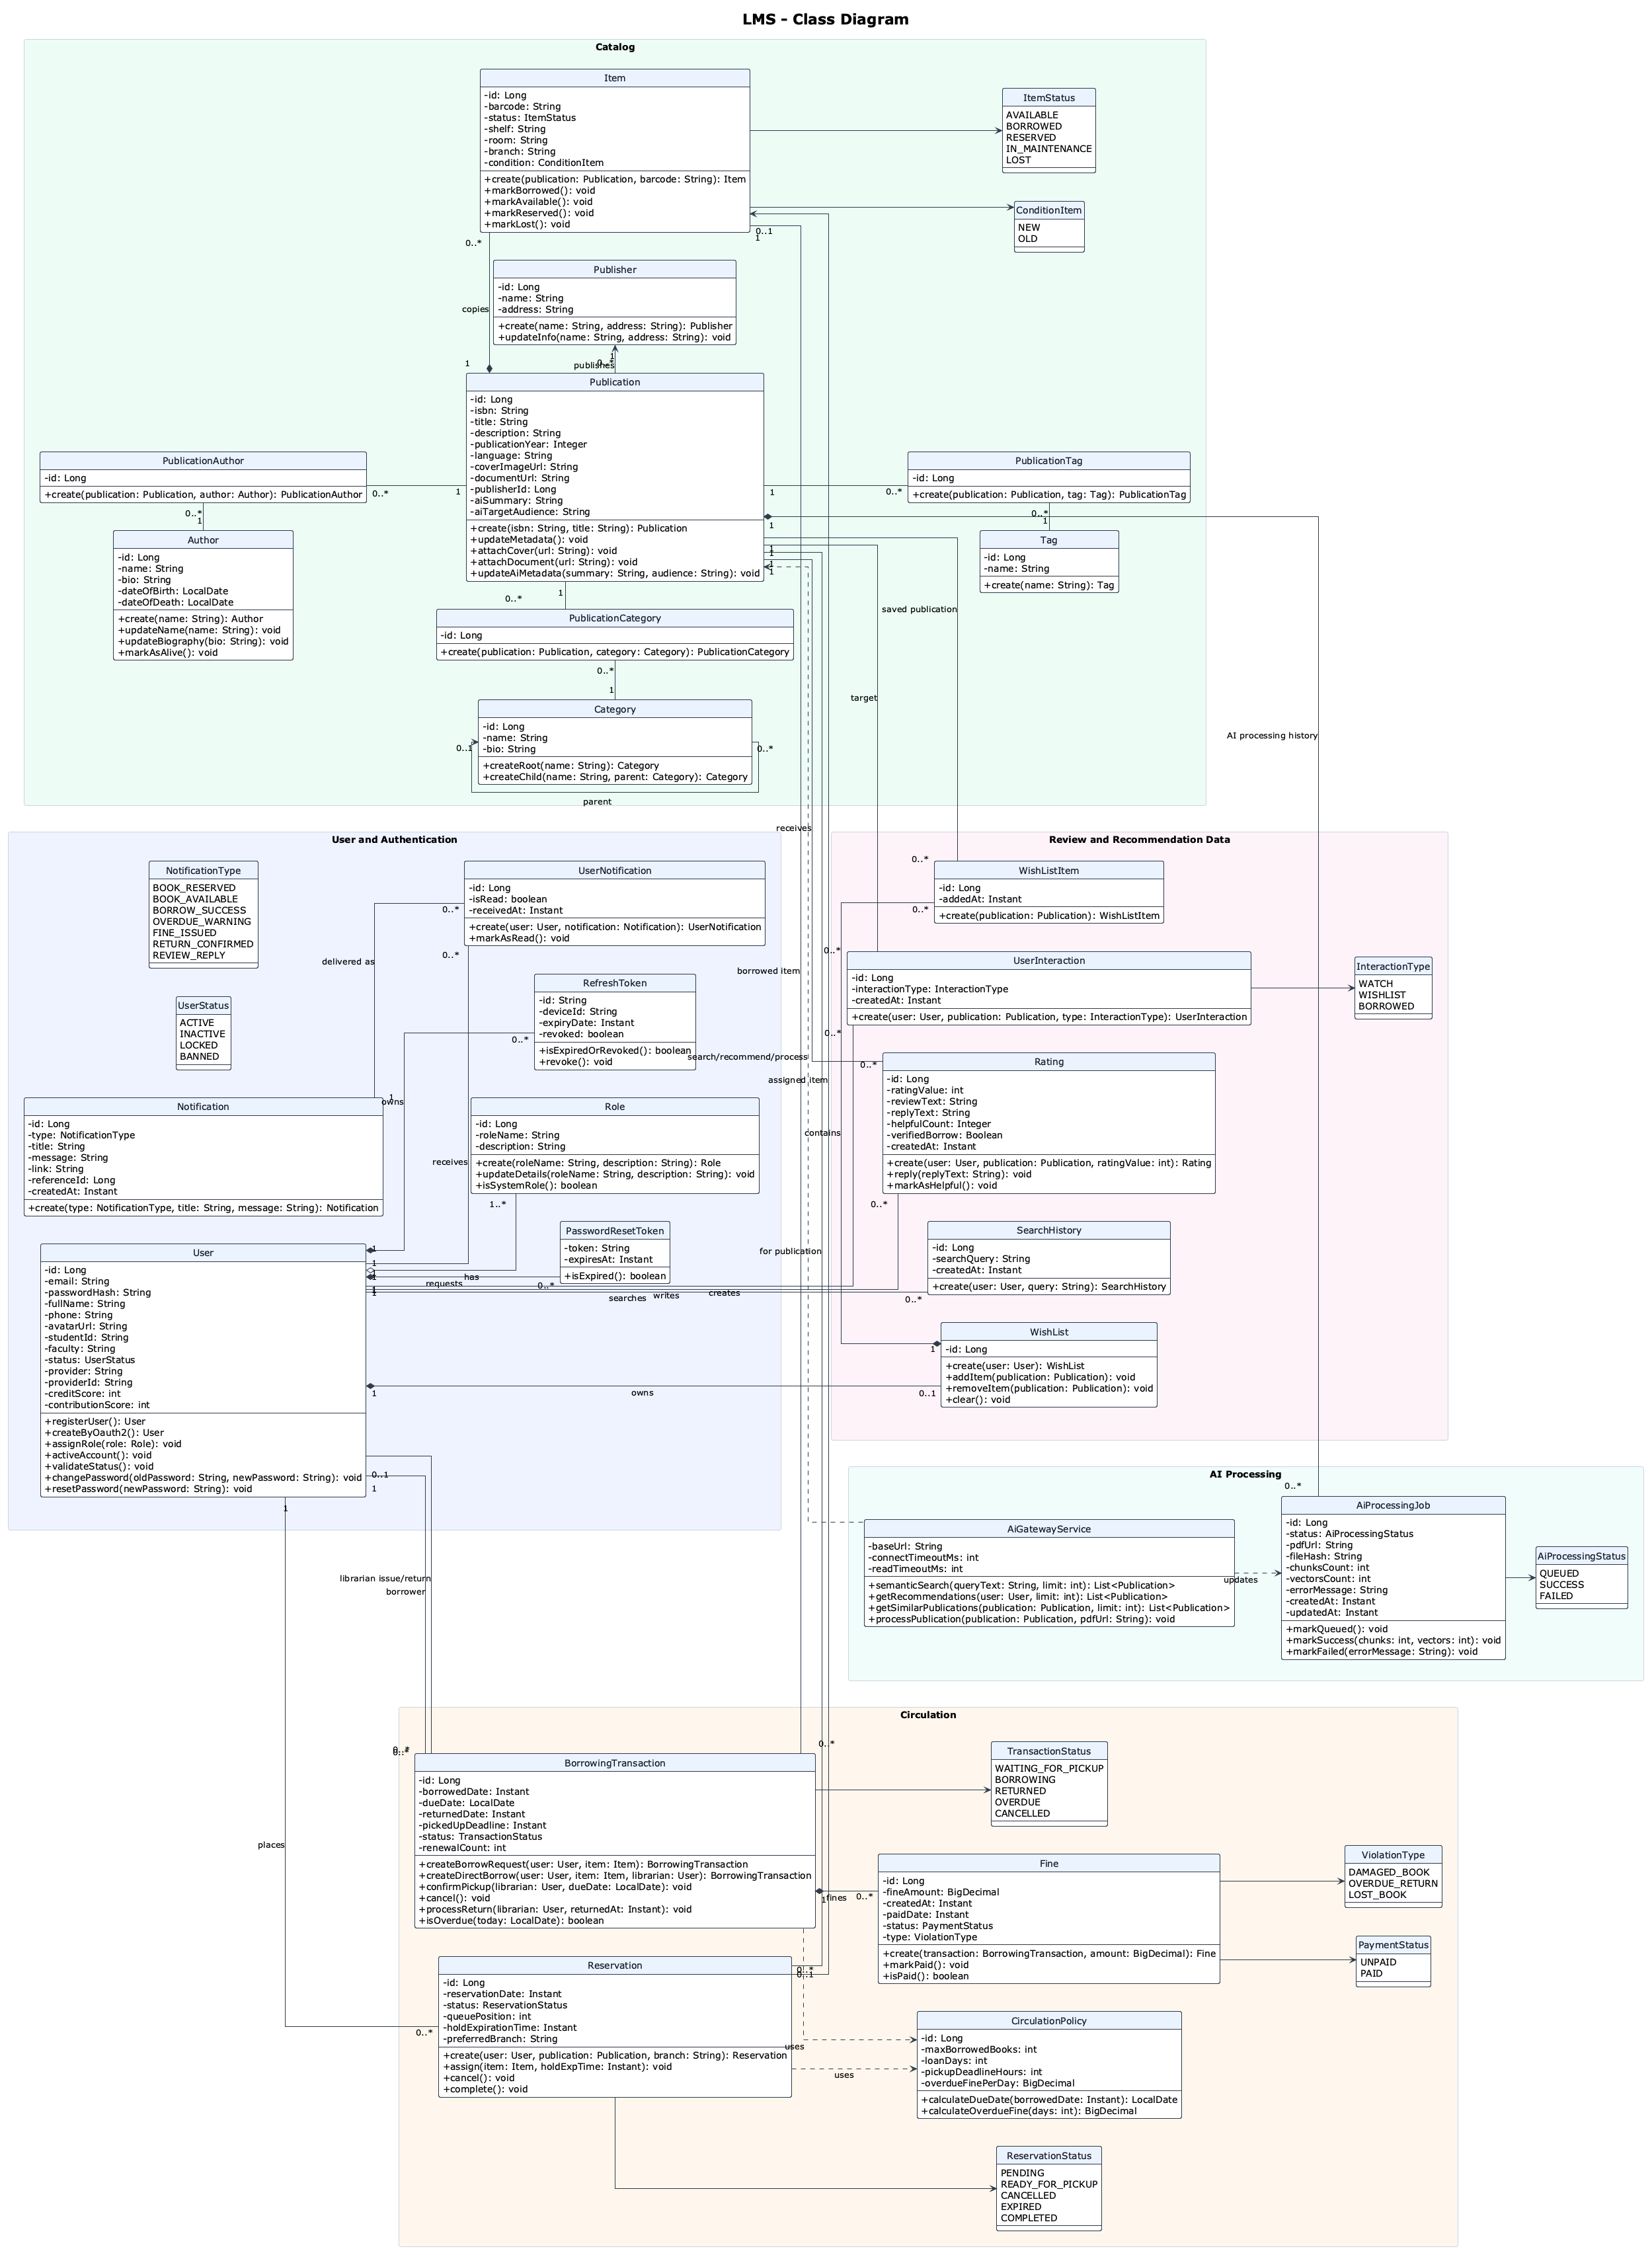
\includegraphics[width=\linewidth, height=0.9\textheight, keepaspectratio]{figures/ch05/class/classdiagram.png}
 \caption{Class diagram tổng quát của hệ thống}
 \label{fig:class_diagram_lms}
\end{figure}

\subsection{Mô hình hoá quy trình nghiệp vụ (Activity diagram)}
\label{subsec:ActivityDiagram}

Các activity diagram trong phần này mô tả những luồng nghiệp vụ đã được hiện thực thành màn hình và API. Riêng chức năng \textbf{gia hạn sách} không được đưa vào phạm vi hiện tại vì backend chưa có use case/controller hoàn chỉnh cho thao tác này; hệ thống chỉ lưu \texttt{renewal\_count} trong mô hình dữ liệu để có thể mở rộng về sau.

% + Đăng ký tài khoản
\begin{figure}[htbp]
 \centering
 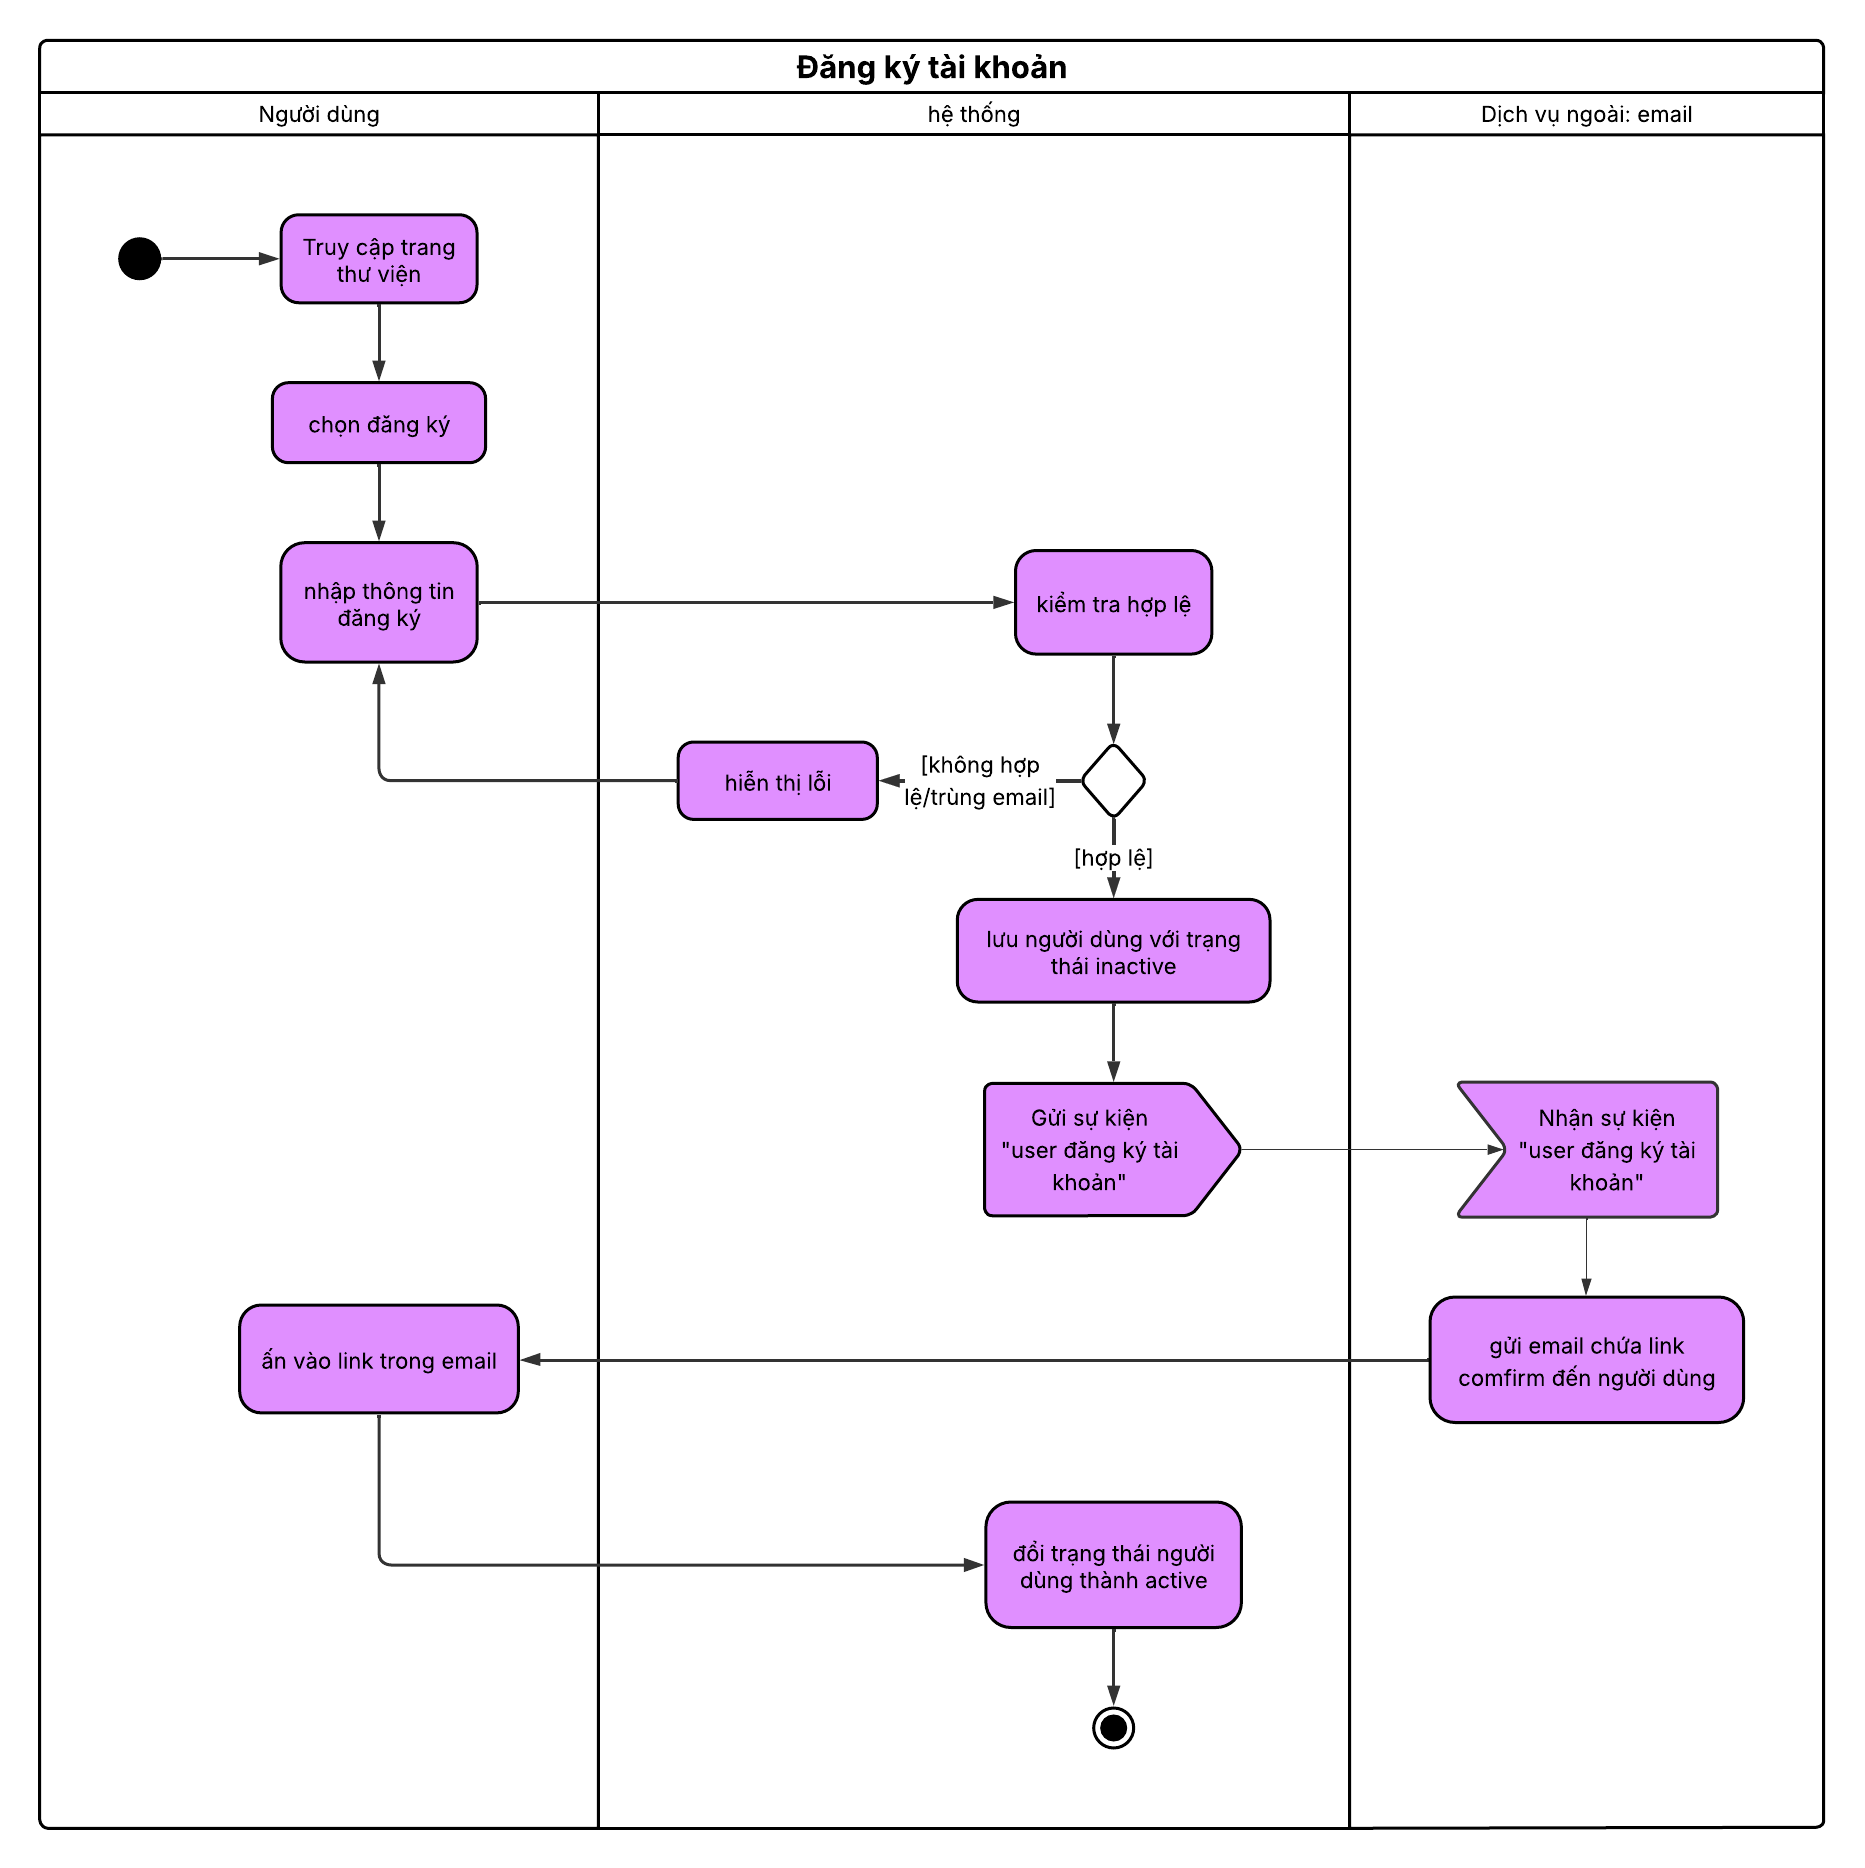
\includegraphics[width=1\linewidth]{figures/ch05/activity/sign_up.png}
 \caption{Đăng ký tài khoản — Activity Diagram}
 \label{fig:signup}
\end{figure}

% + Đăng nhập tài khoản
\begin{figure}[htbp]
 \centering
 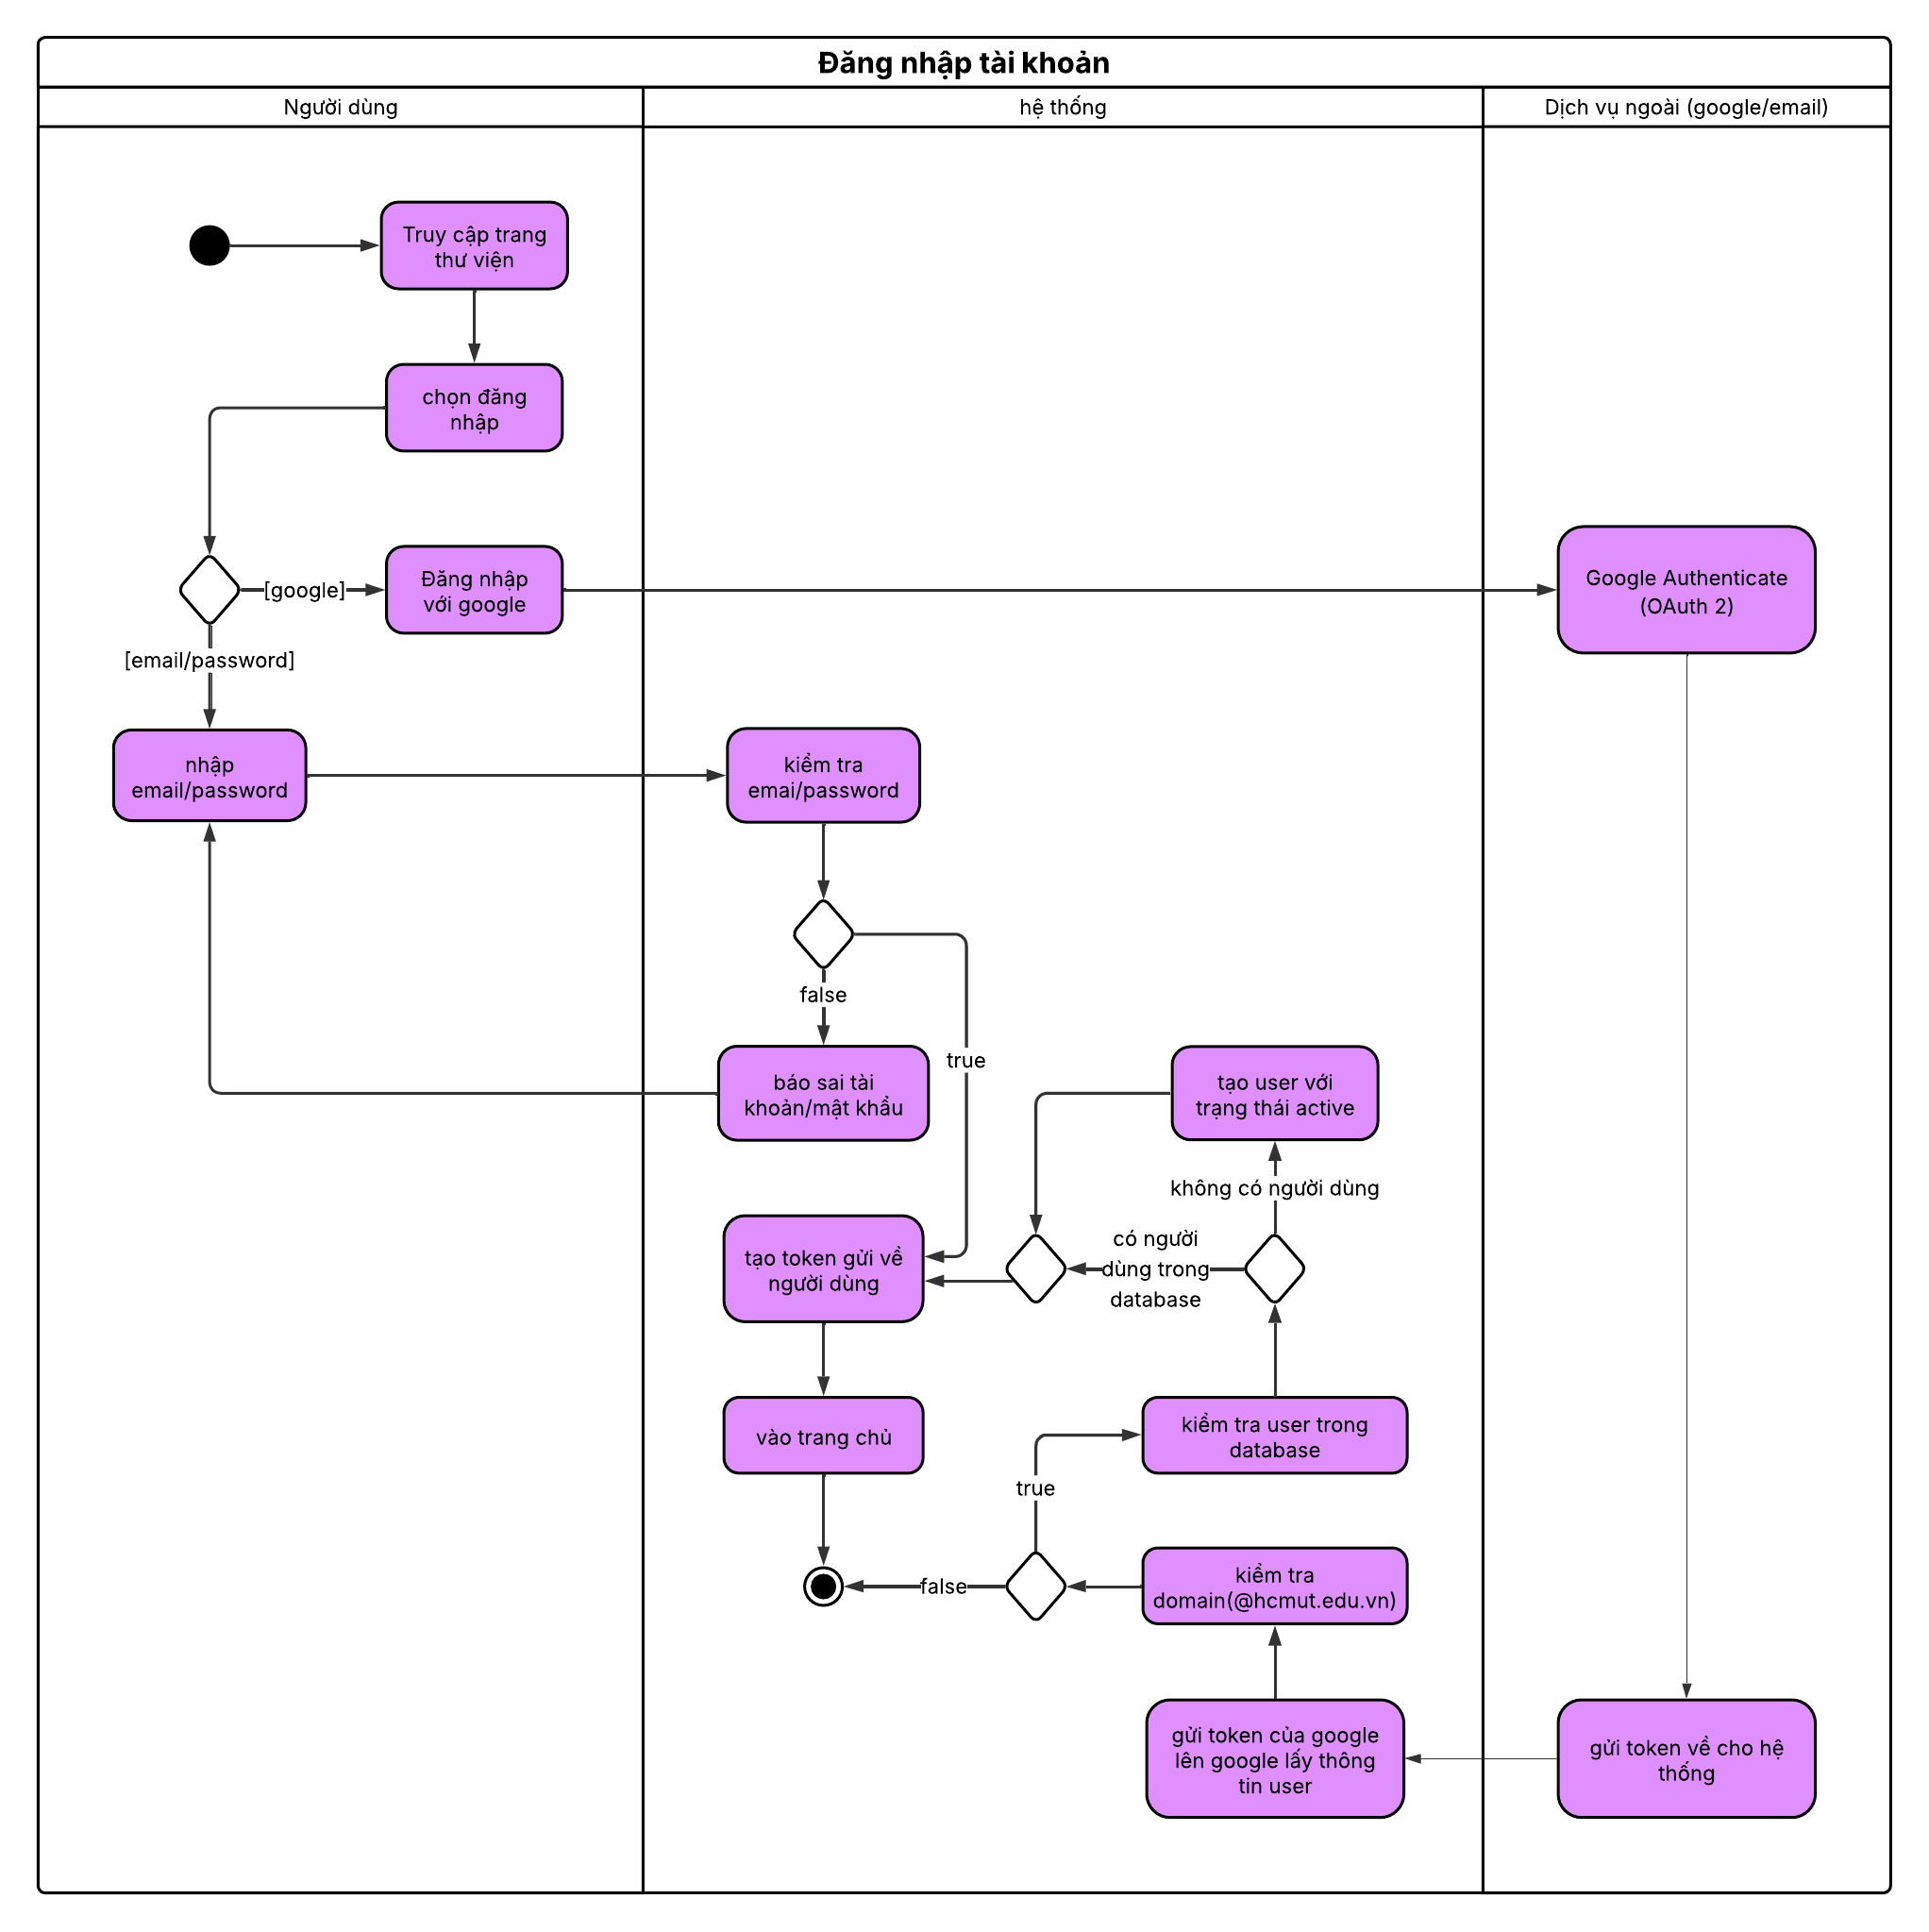
\includegraphics[width=1\linewidth]{figures/ch05/activity/login.png}
 \caption{Đăng nhập tài khoản — Activity Diagram}
 \label{fig:signin}
\end{figure}

% + Tìm kiếm sách:
\begin{figure}[htbp]
 \centering
 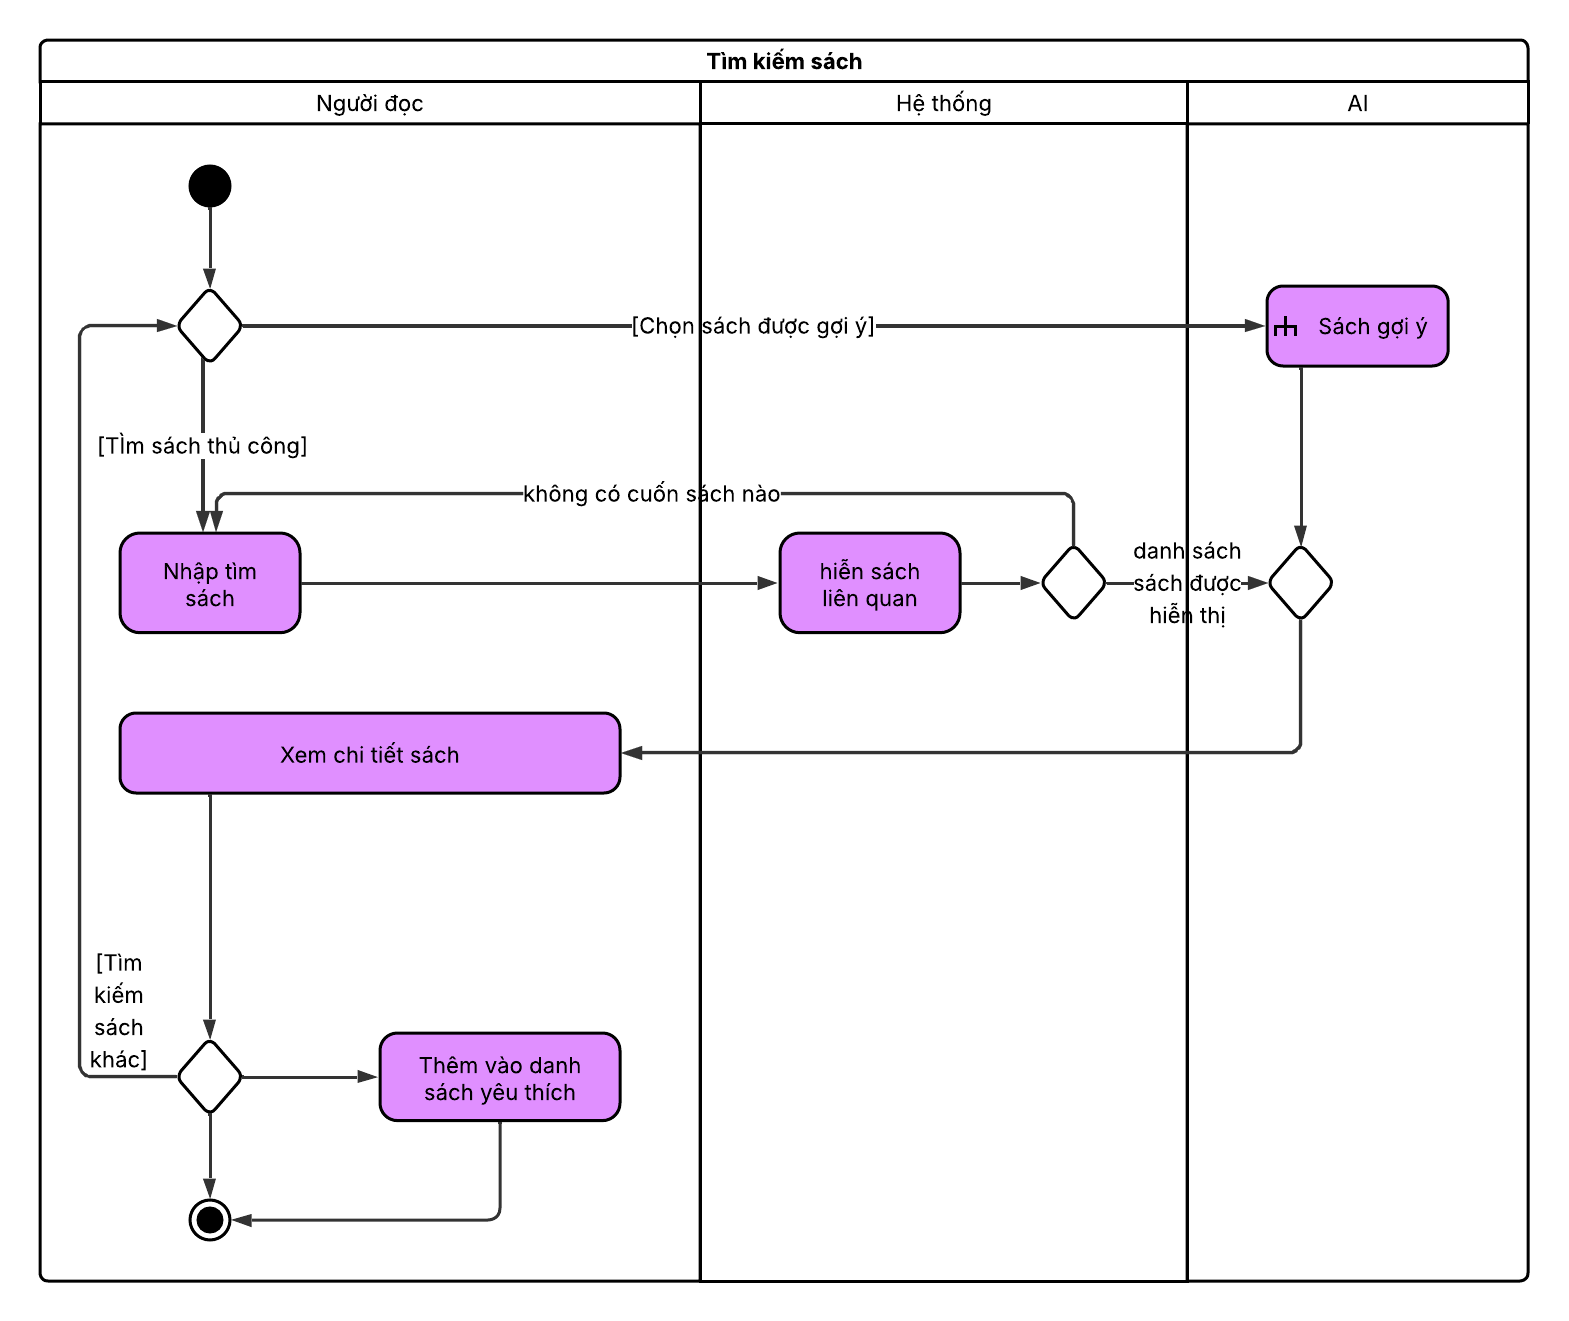
\includegraphics[width=\linewidth]{figures/ch05/activity/search_book.png}
 \caption{Tìm kiếm sách — Activity Diagram}
 \label{fig:search-book}
\end{figure}

% + Gợi ý sách:
\begin{figure}[htbp]
 \centering
 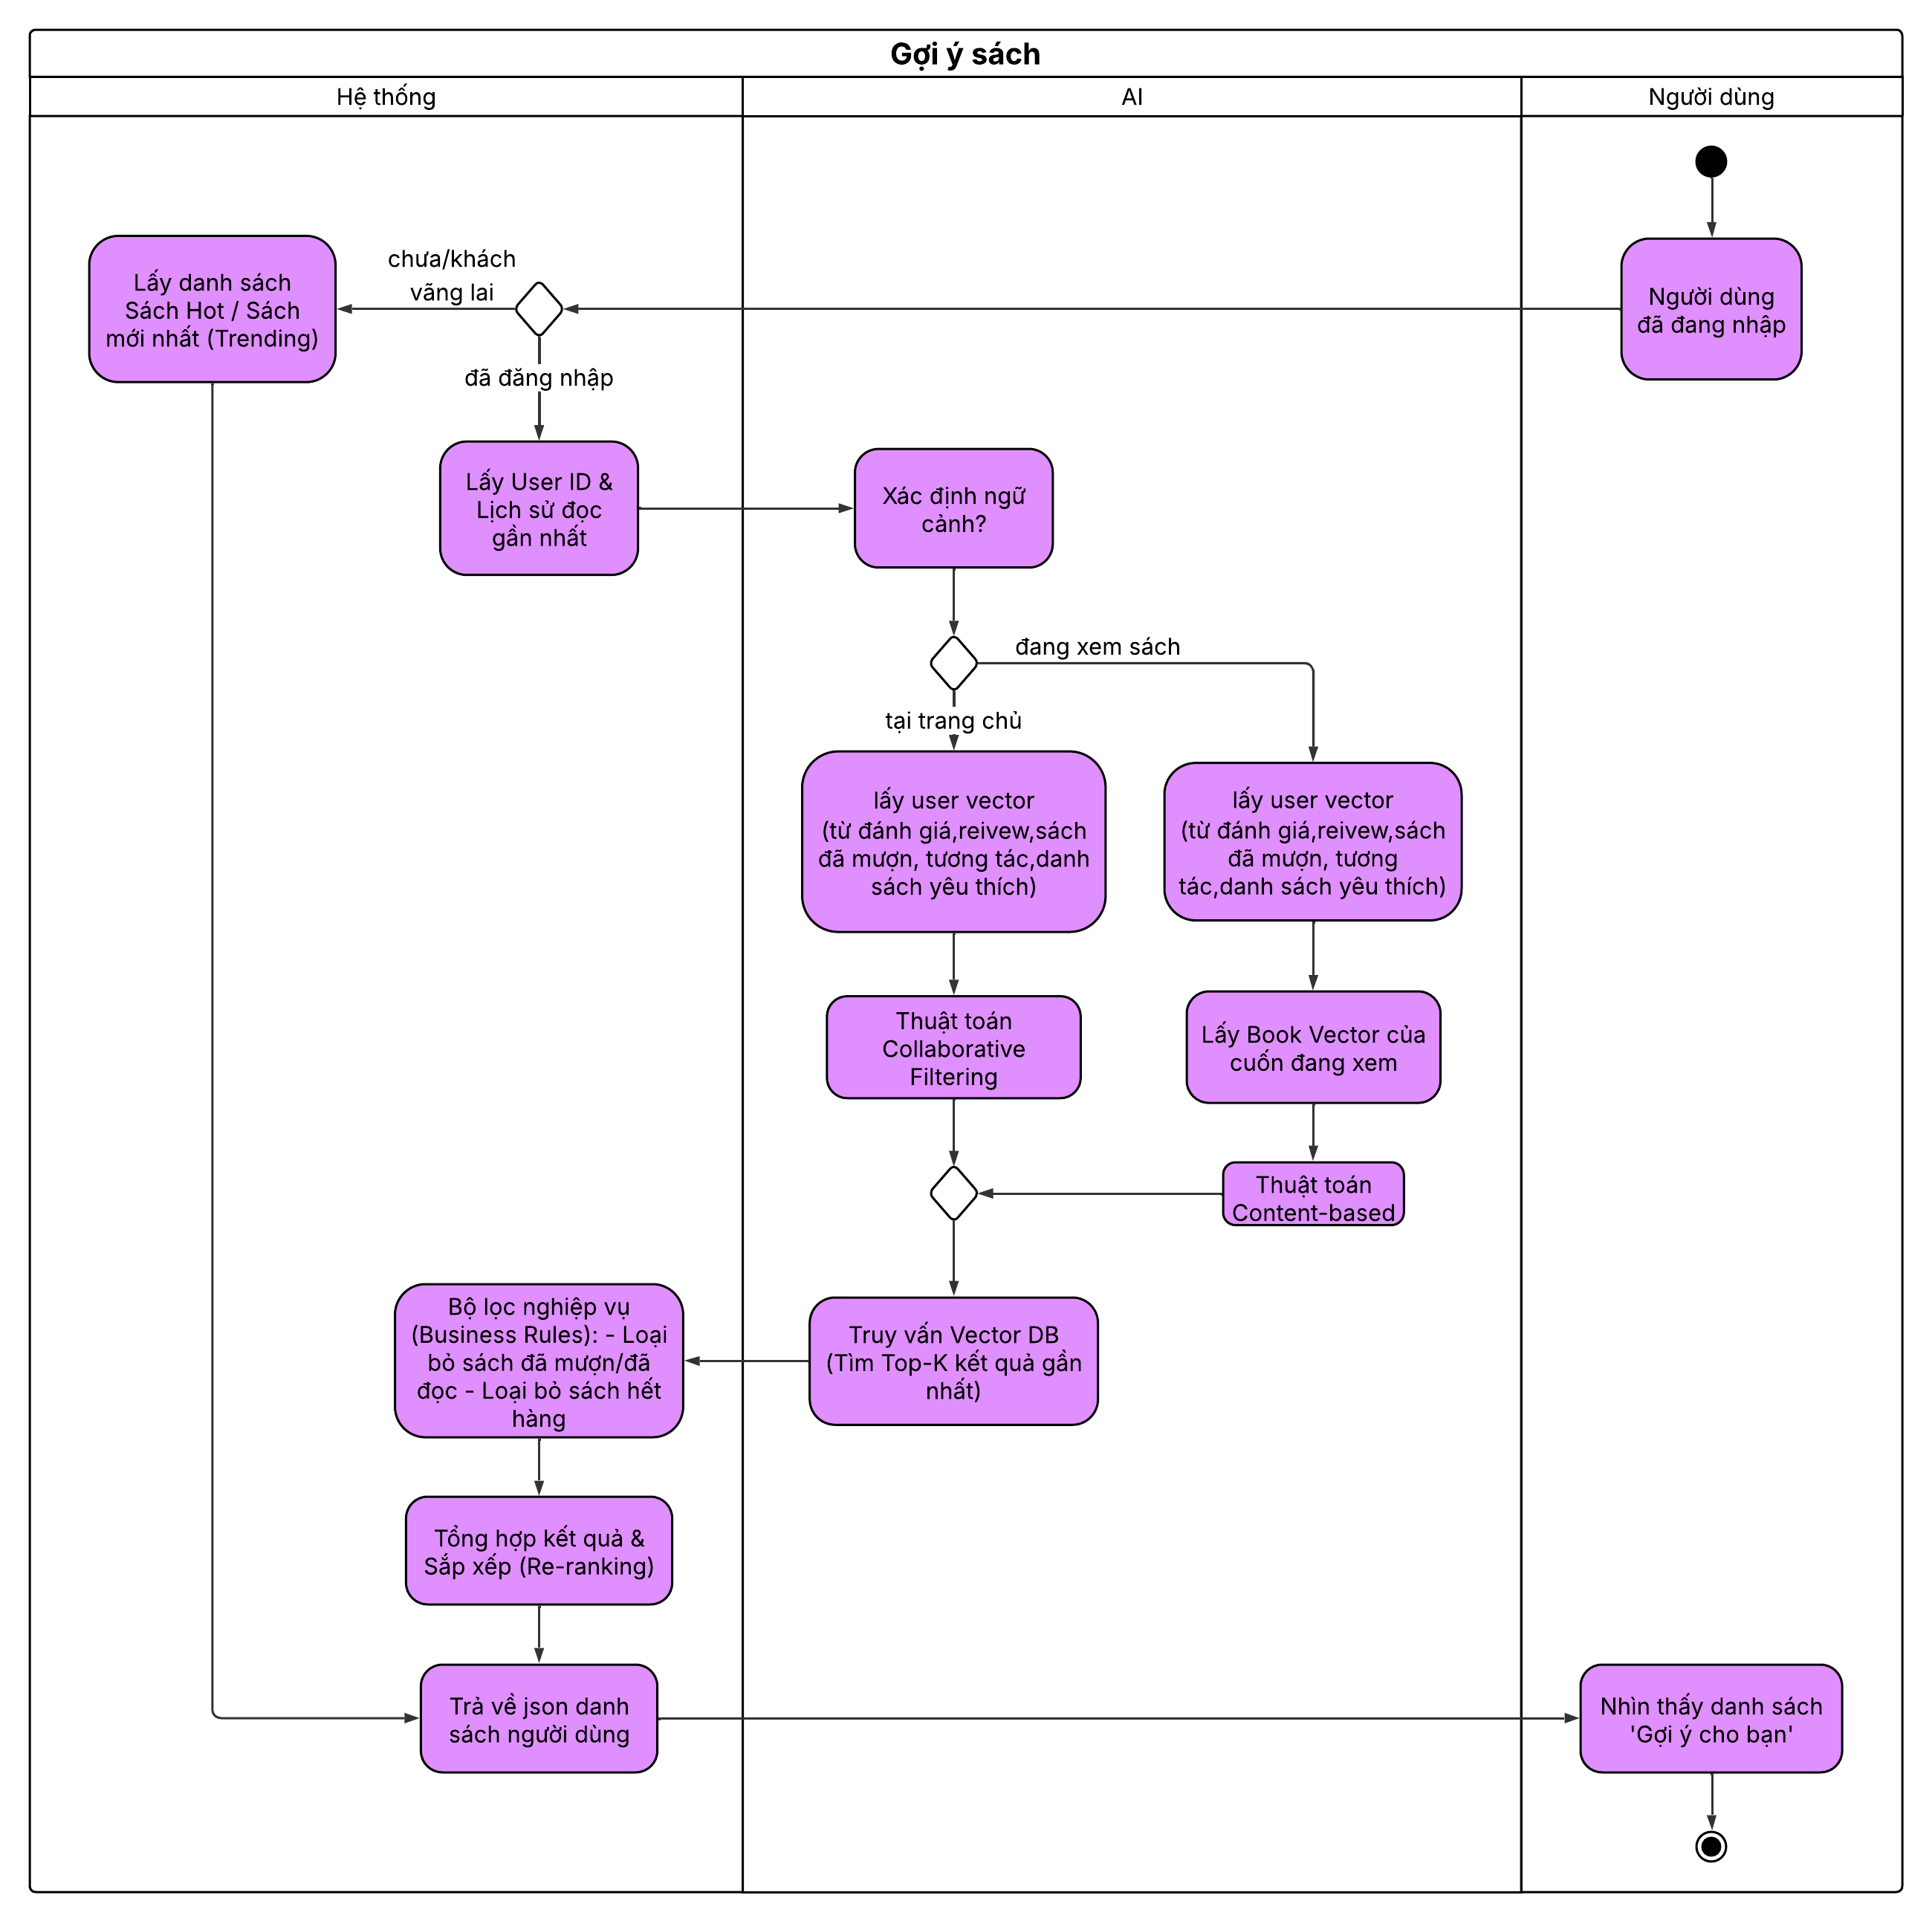
\includegraphics[width=\linewidth]{figures/ch05/activity/suggest_book.png}
 \caption{Gợi ý sách — Activity Diagram}
 \label{fig:suggestion}
\end{figure}

\begin{figure}[htbp]
 \centering
 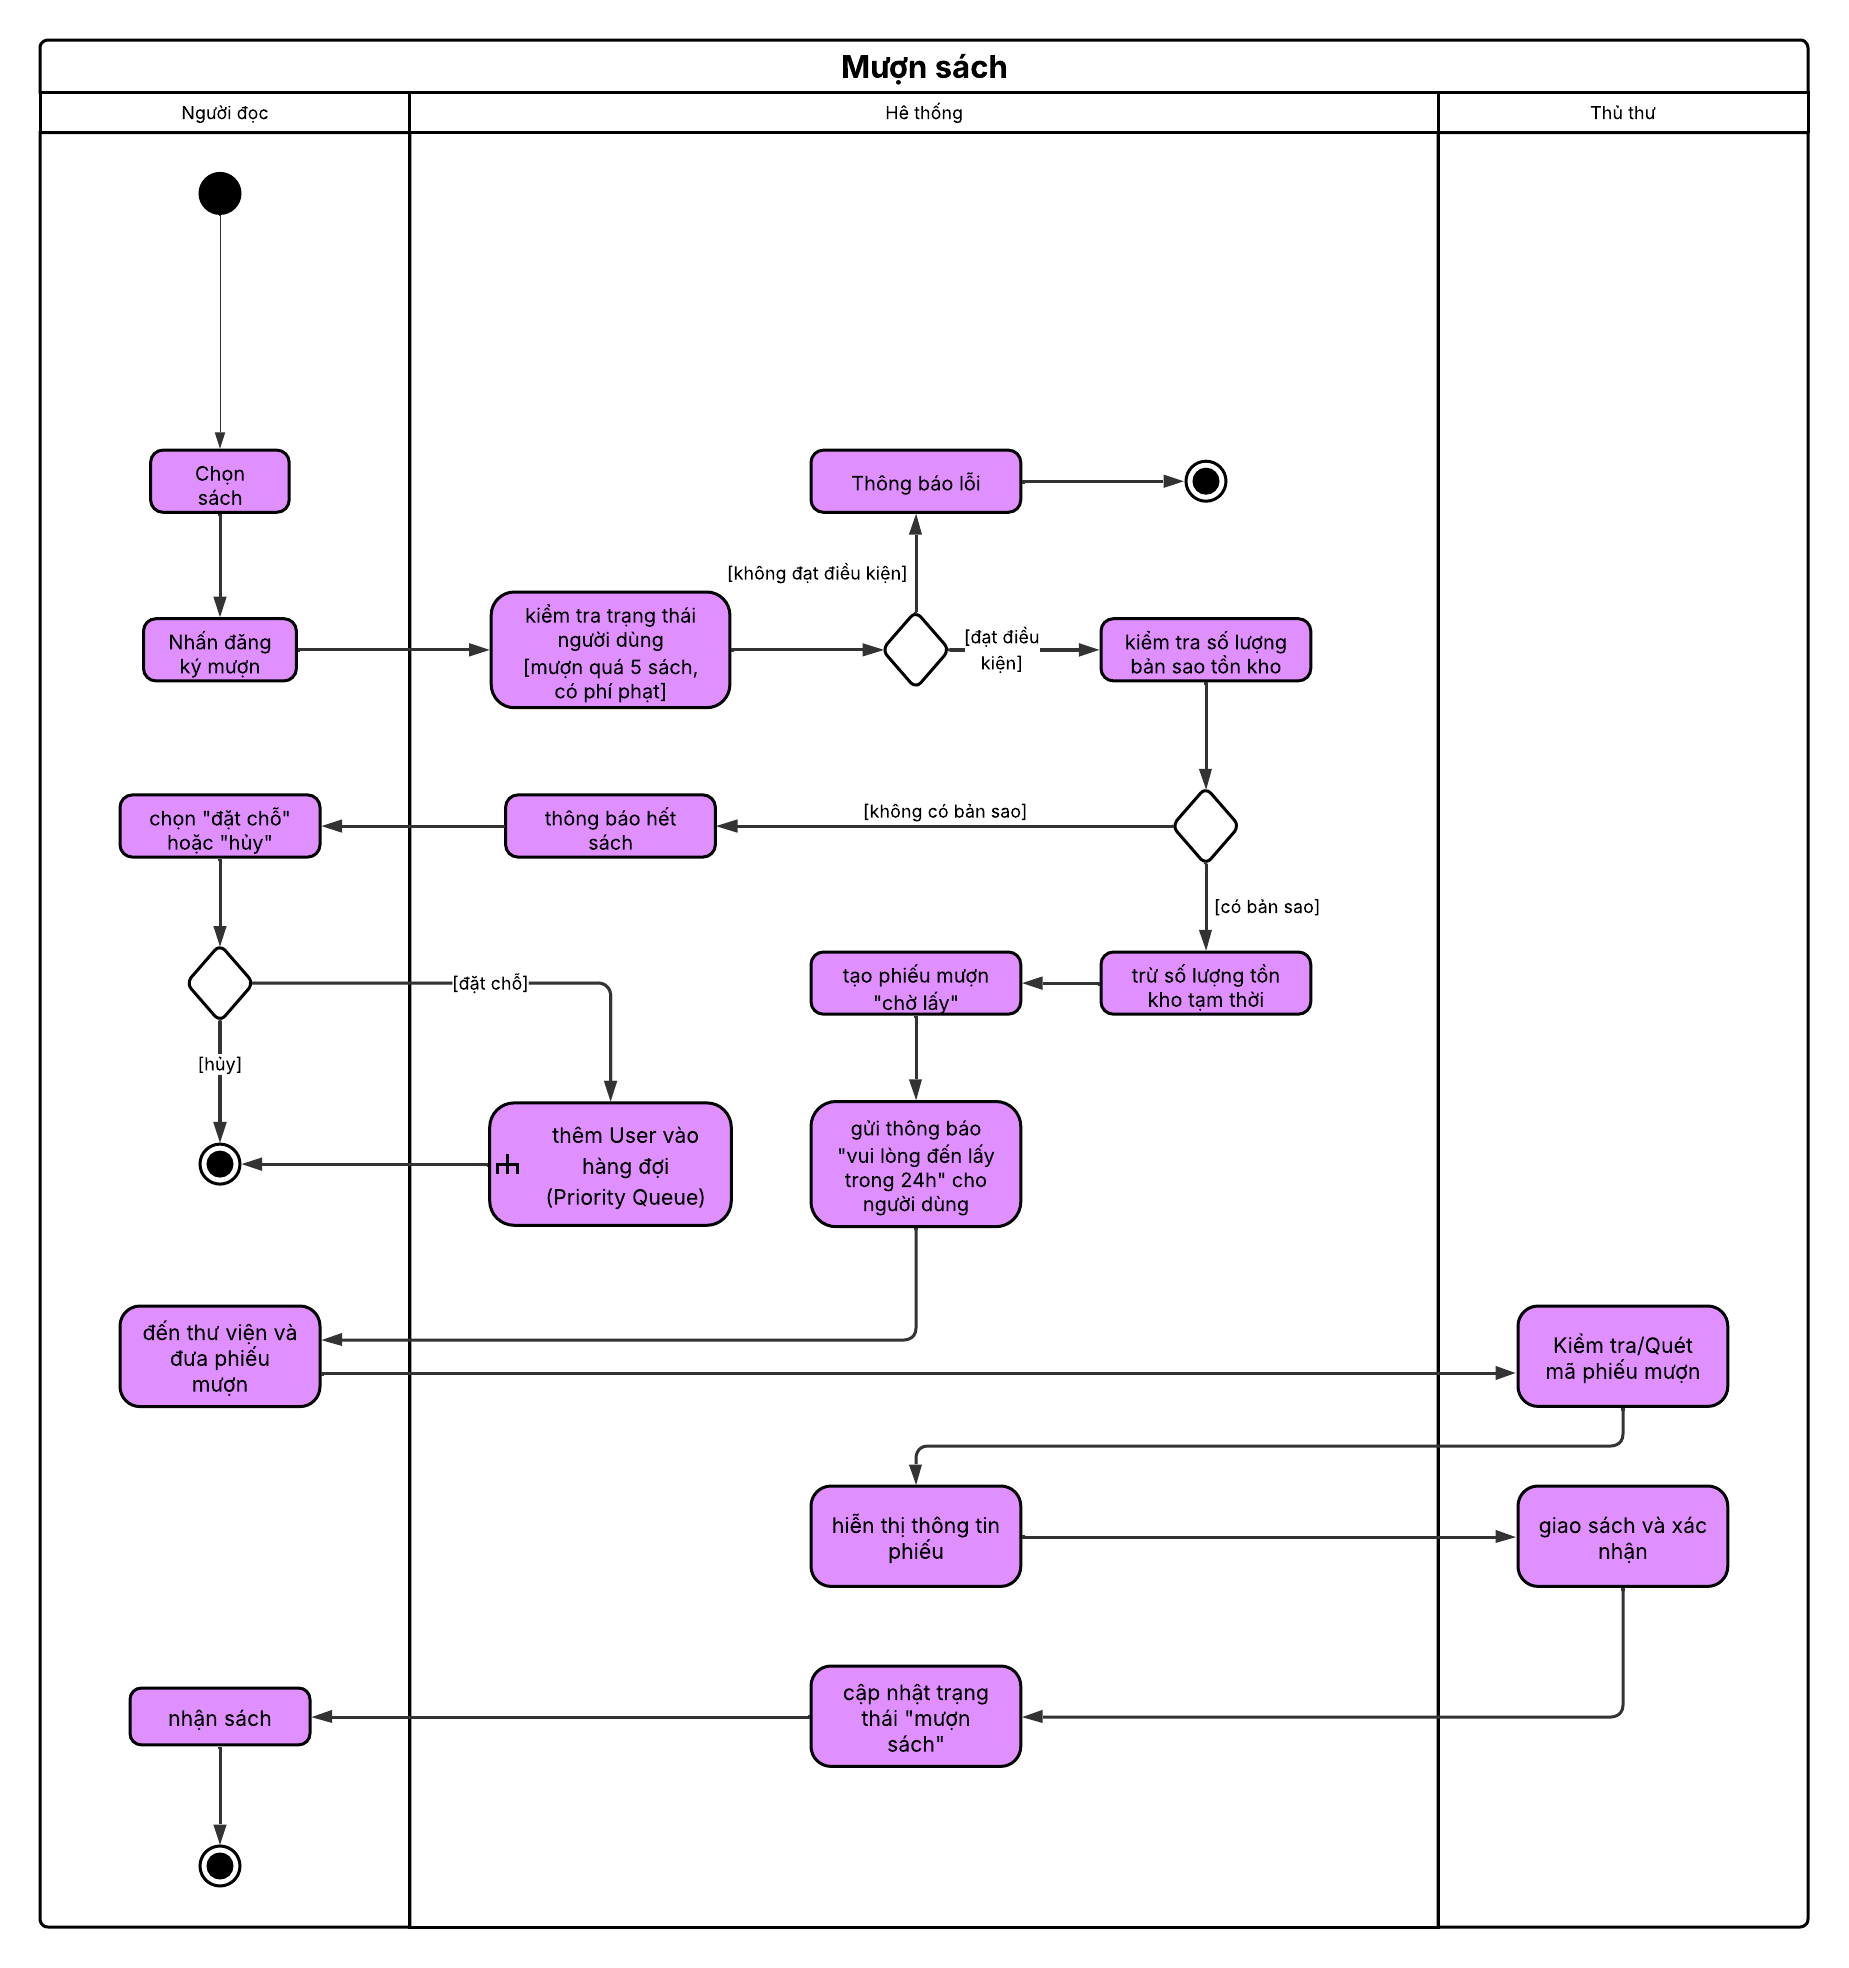
\includegraphics[width=\linewidth]{figures/ch05/activity/borrow_book.png}
 \caption{Mượn sách — Activity Diagram}
 \label{fig:borrow_book}
\end{figure}

\begin{figure}[htbp]
 \centering
 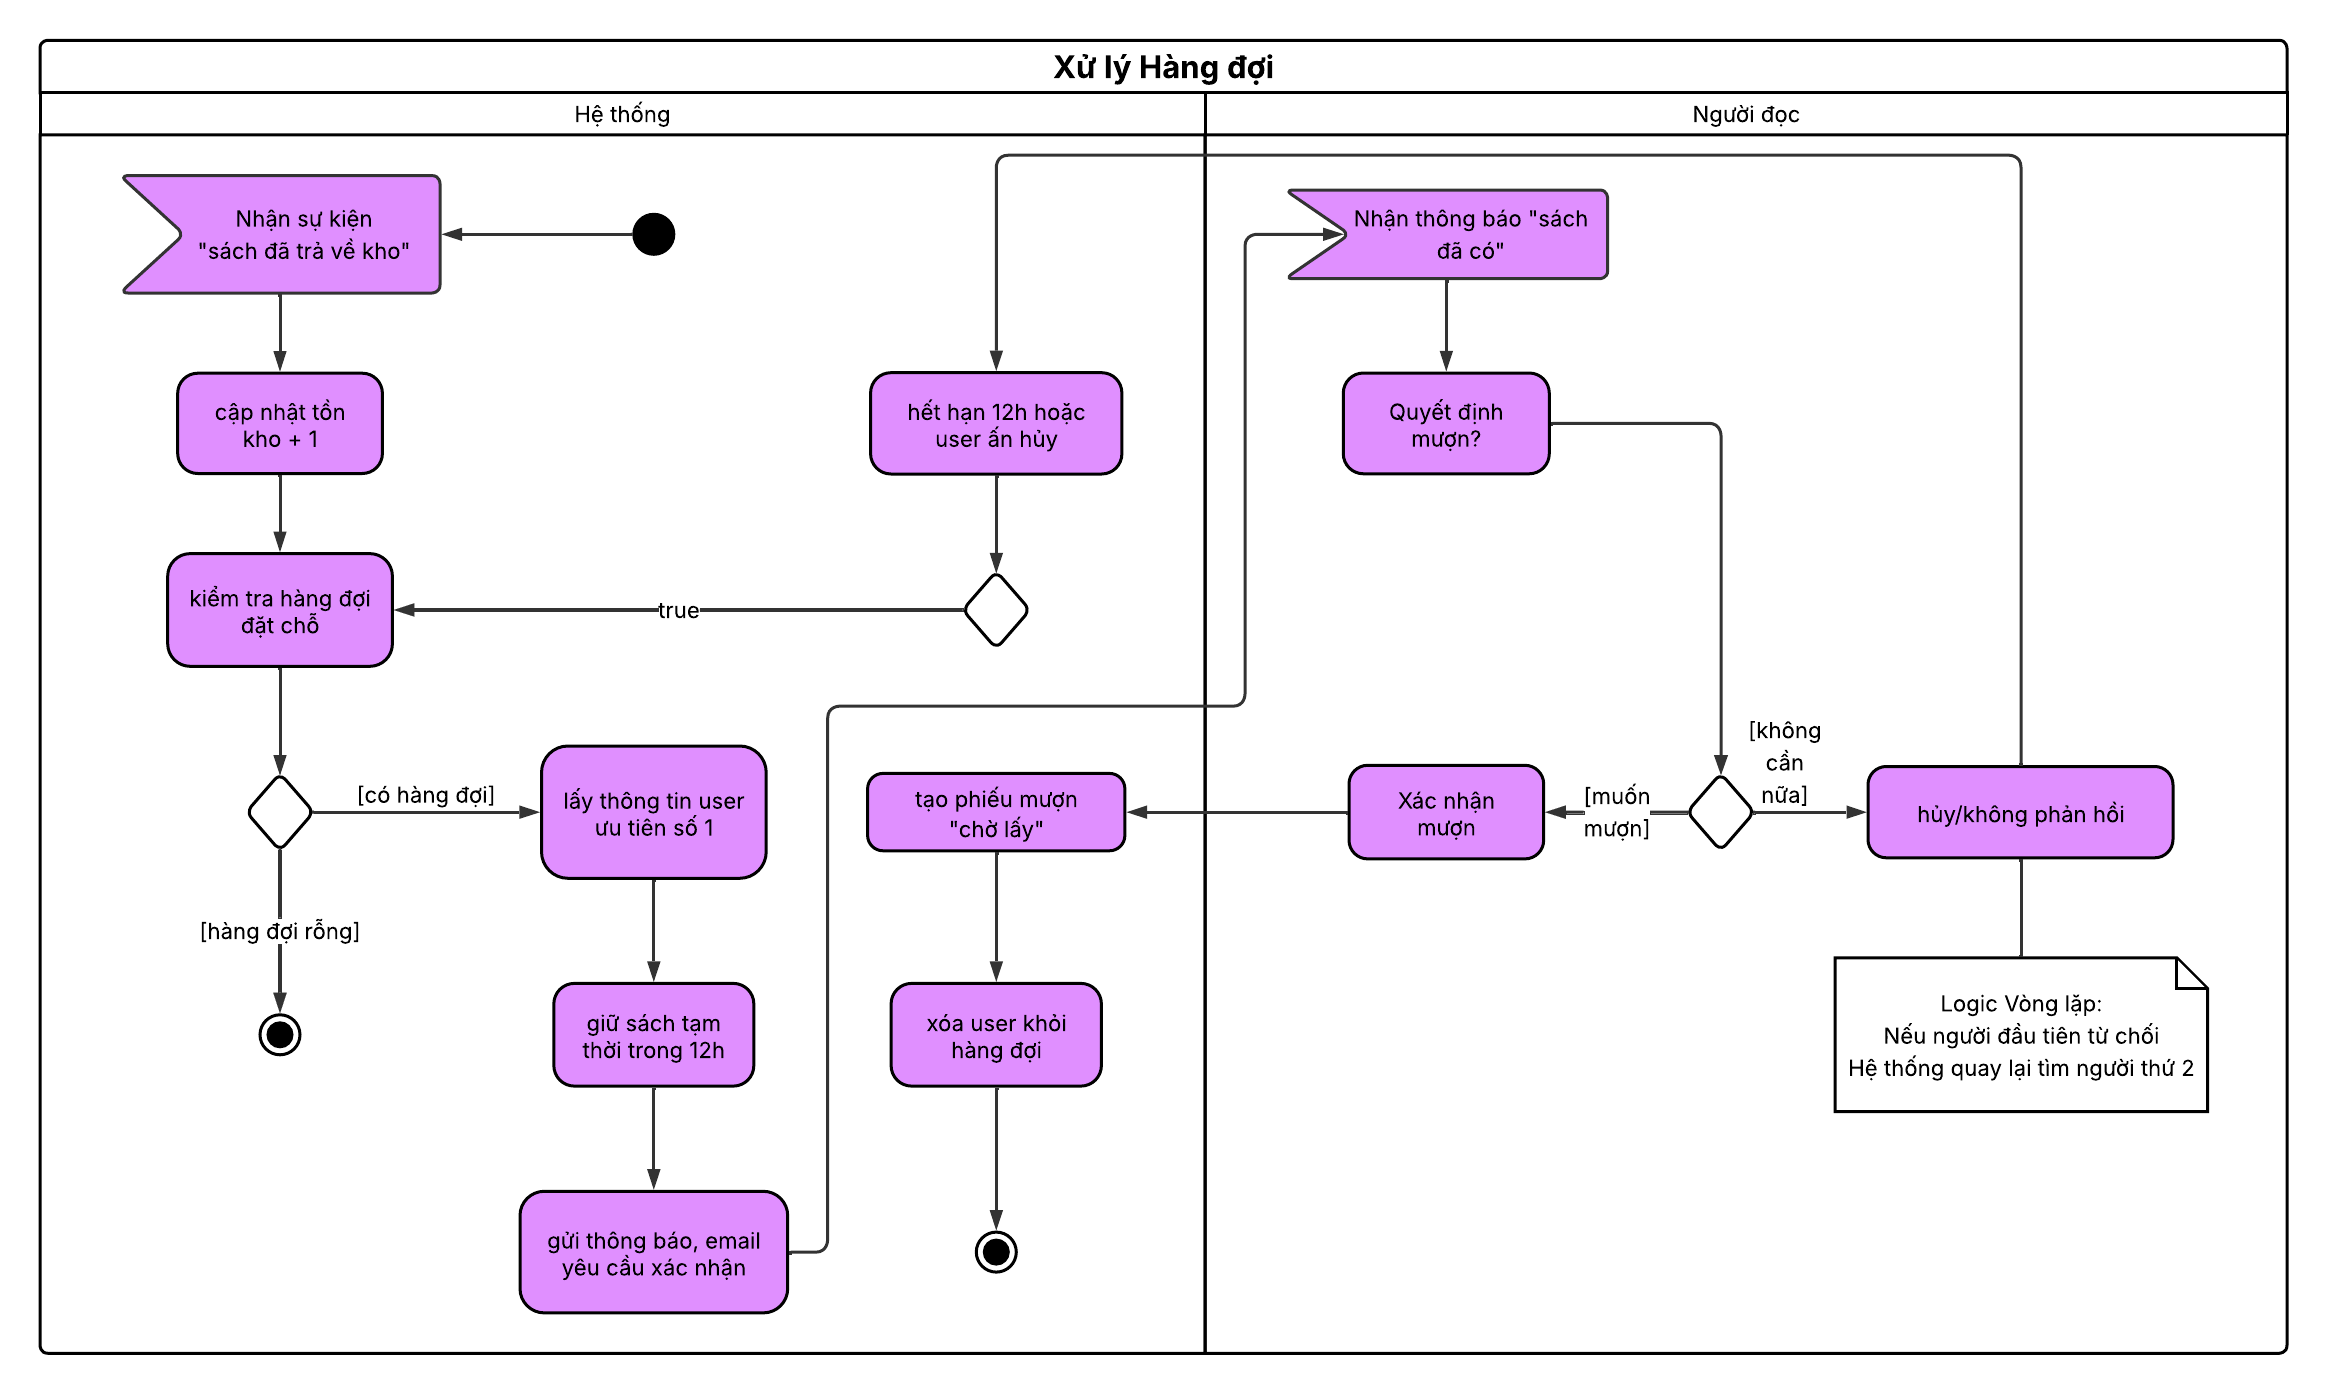
\includegraphics[width=\linewidth]{figures/ch05/activity/process_queue.png}
 \caption{Xử lý hàng đợi đặt trước — Activity Diagram}
 \label{fig:process_queue}
\end{figure}

\begin{figure}[htbp]
 \centering
 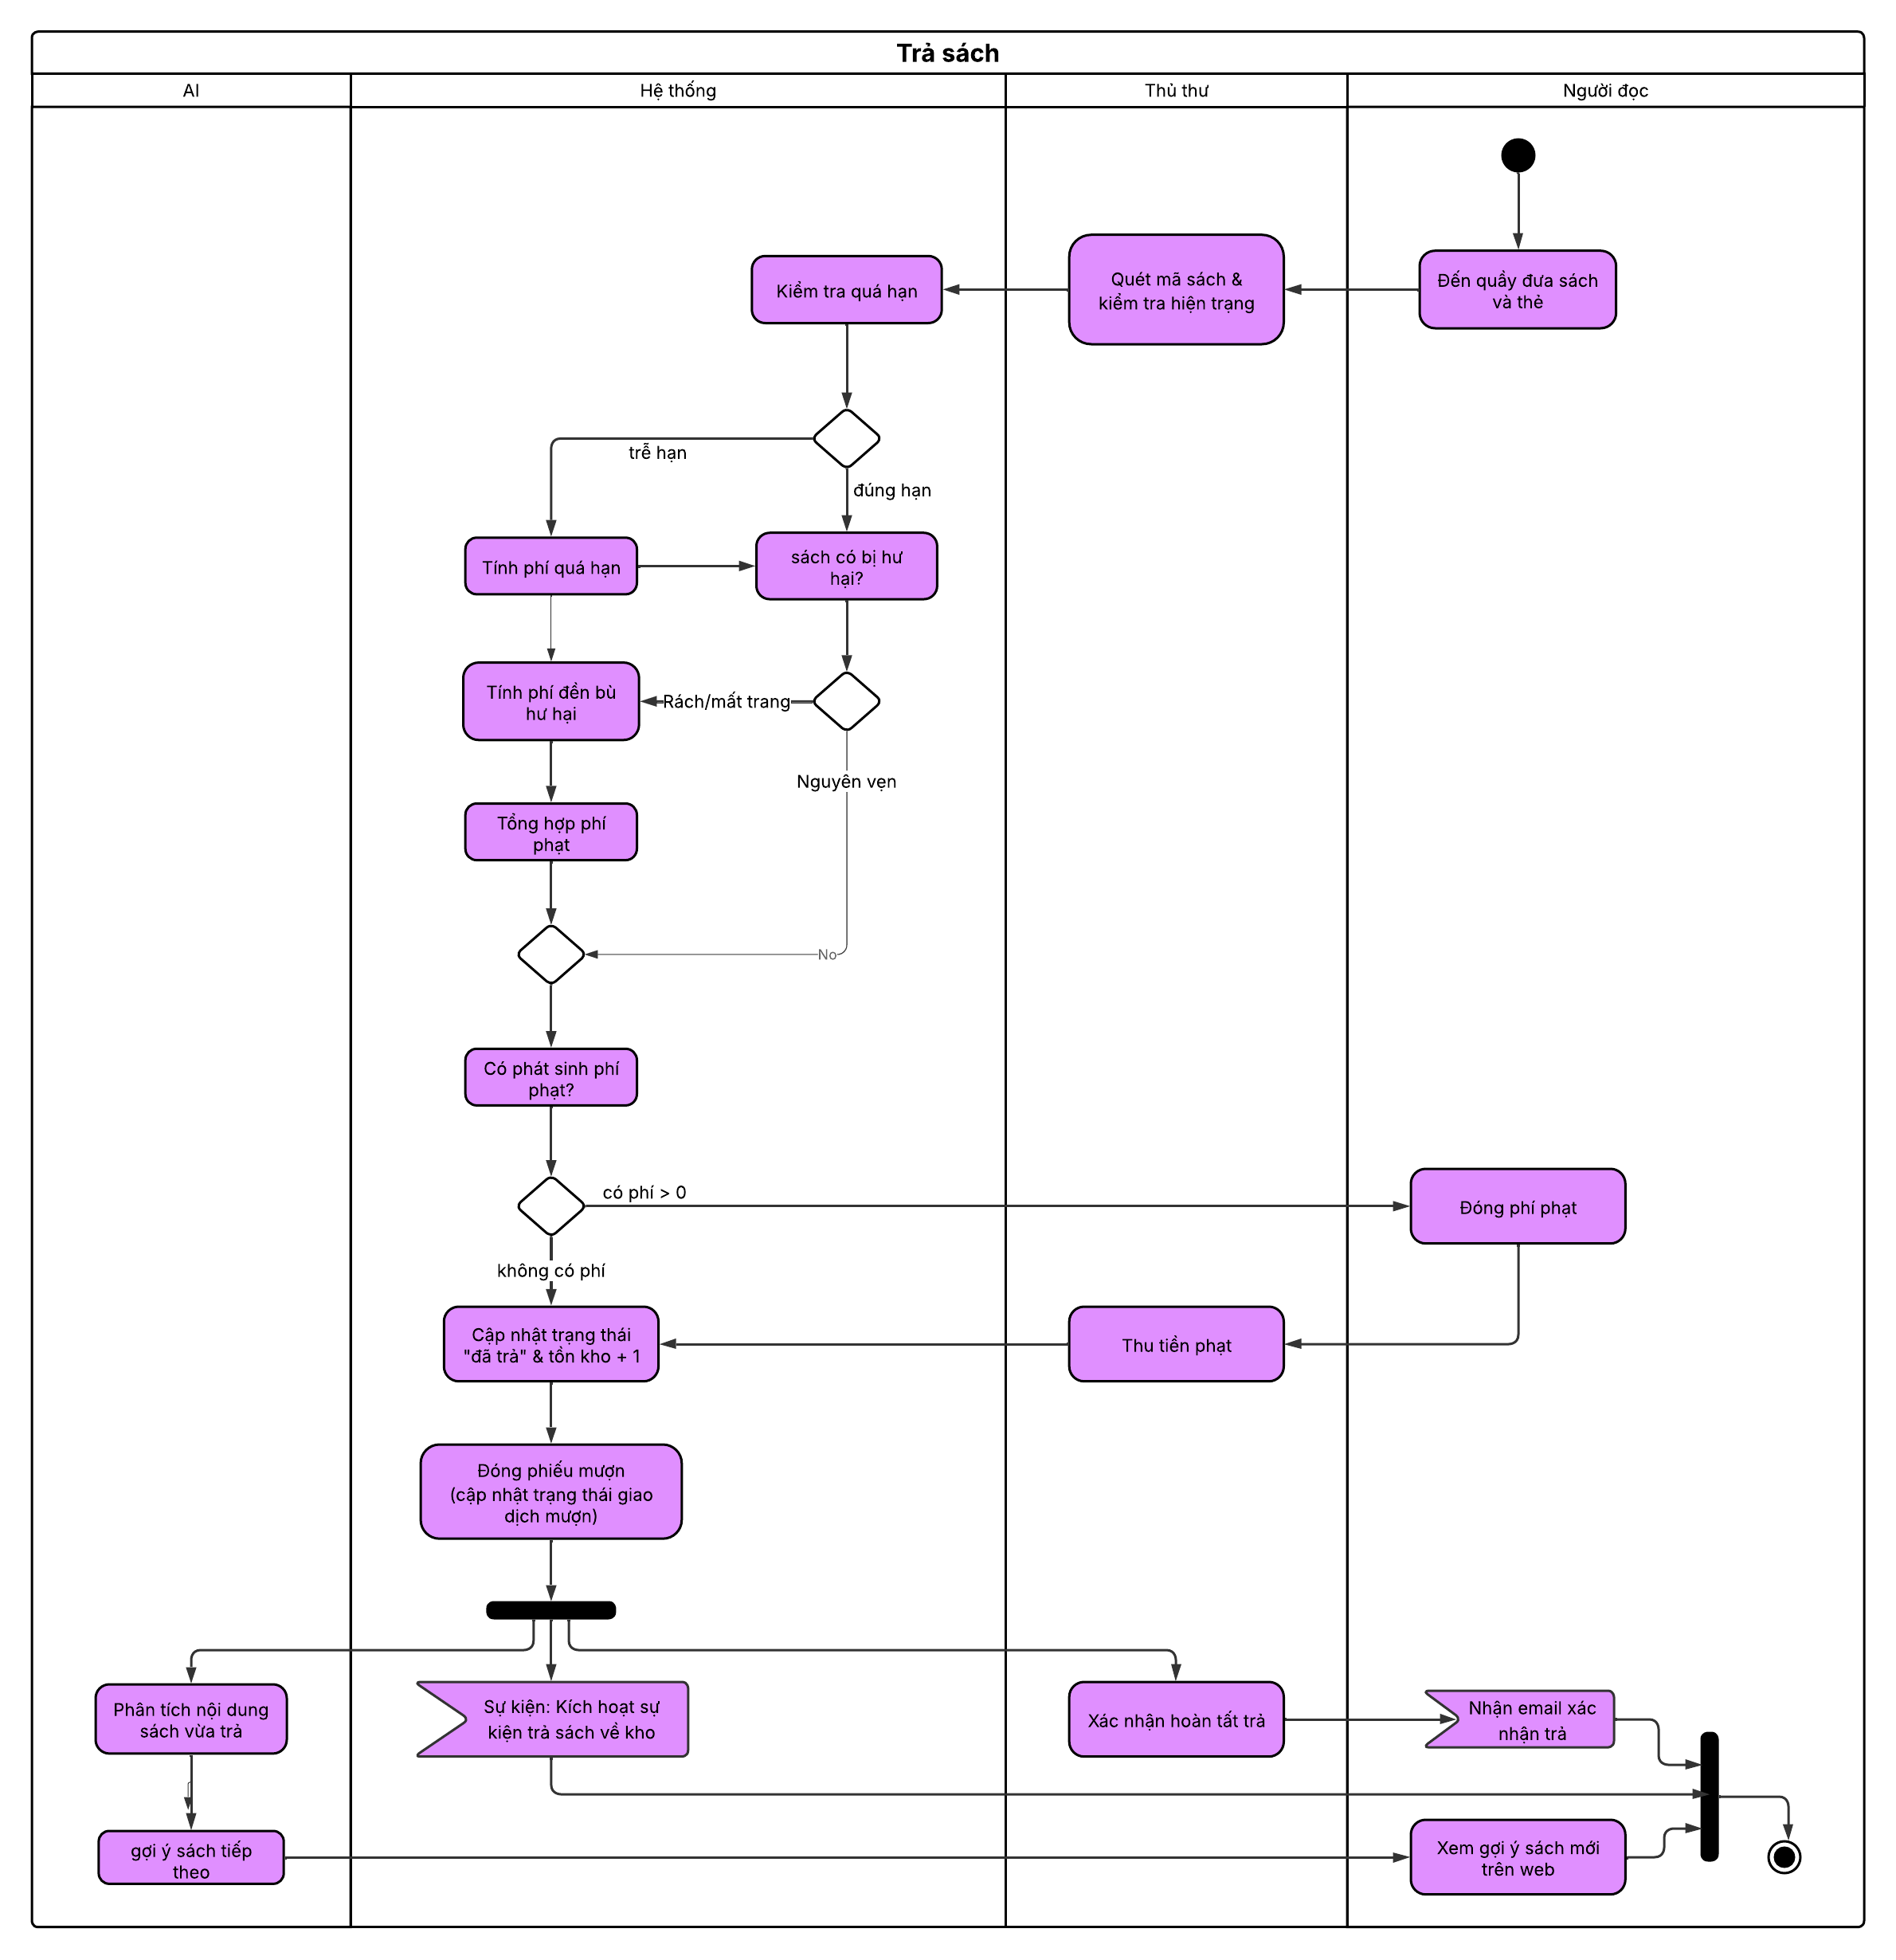
\includegraphics[width=\linewidth]{figures/ch05/activity/return_book.png}
 \caption{Trả sách — Activity Diagram}
 \label{fig:return_book}
\end{figure}

\begin{figure}[htbp]
 \centering
 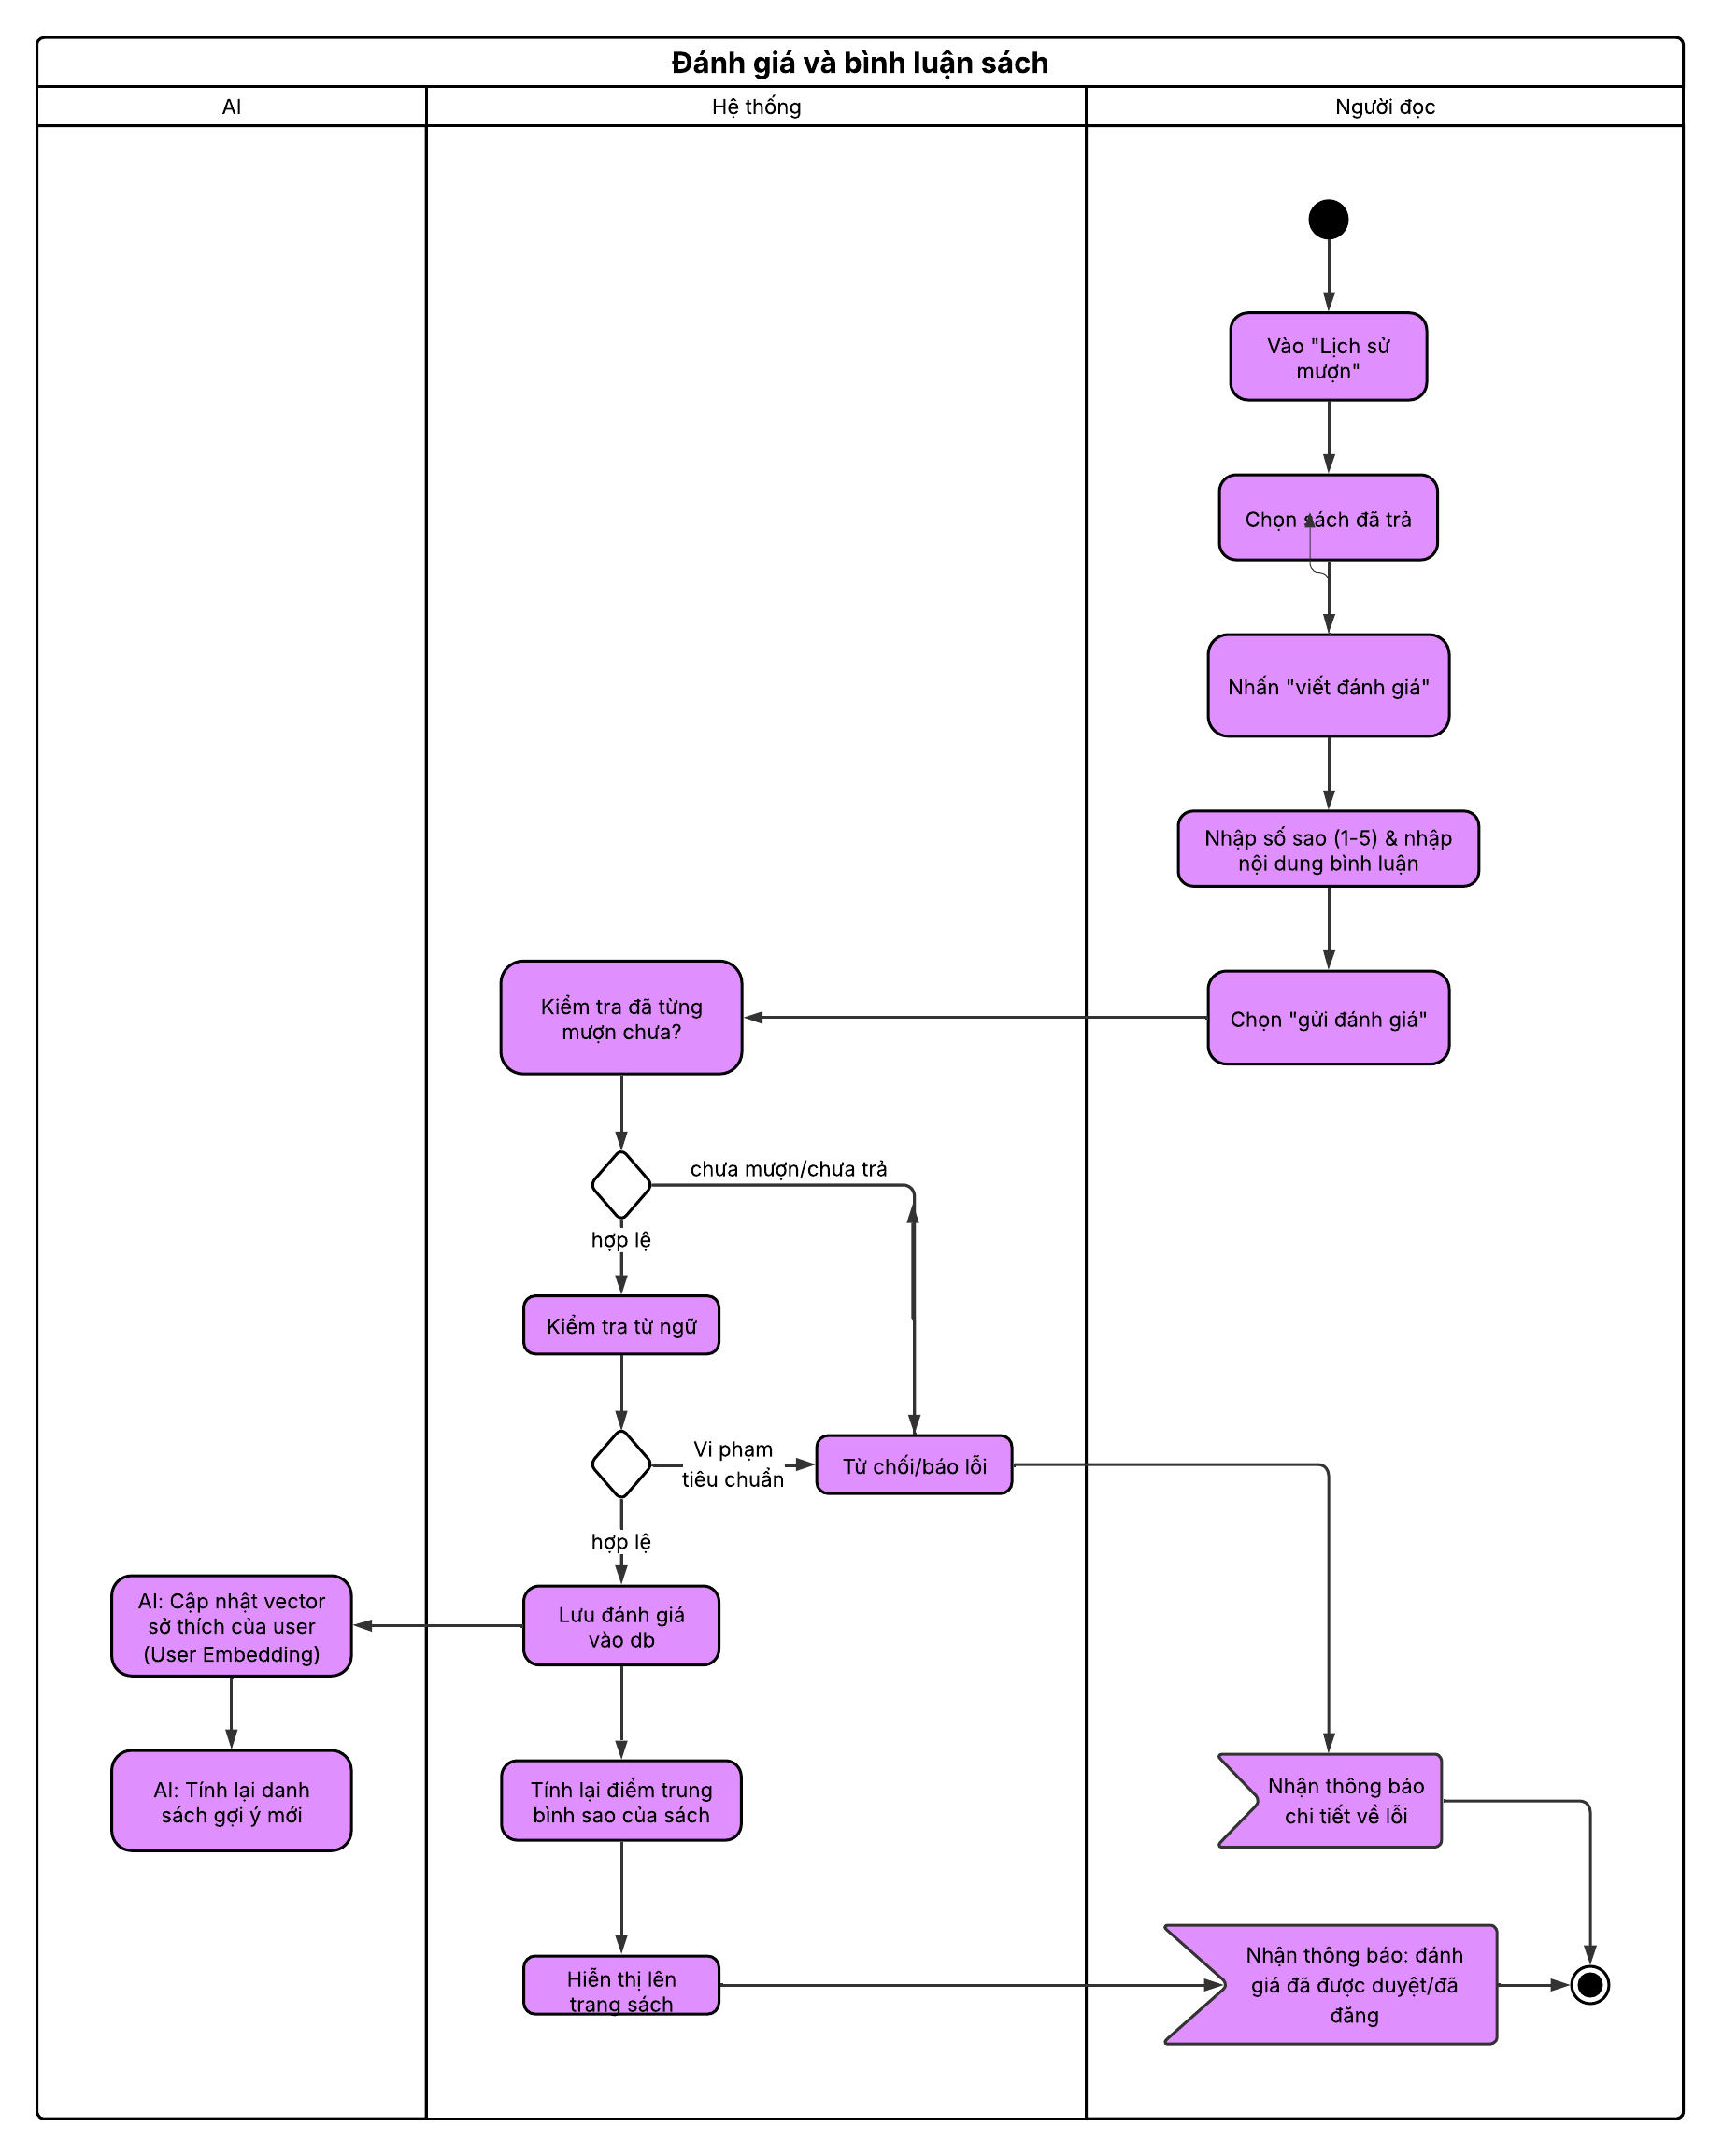
\includegraphics[width=\linewidth]{figures/ch05/activity/review_and_comment.png}
 \caption{Đánh giá và bình luận sách — Activity Diagram}
 \label{fig:book_review_comment}
\end{figure}

\begin{figure}[htbp]
 \centering
 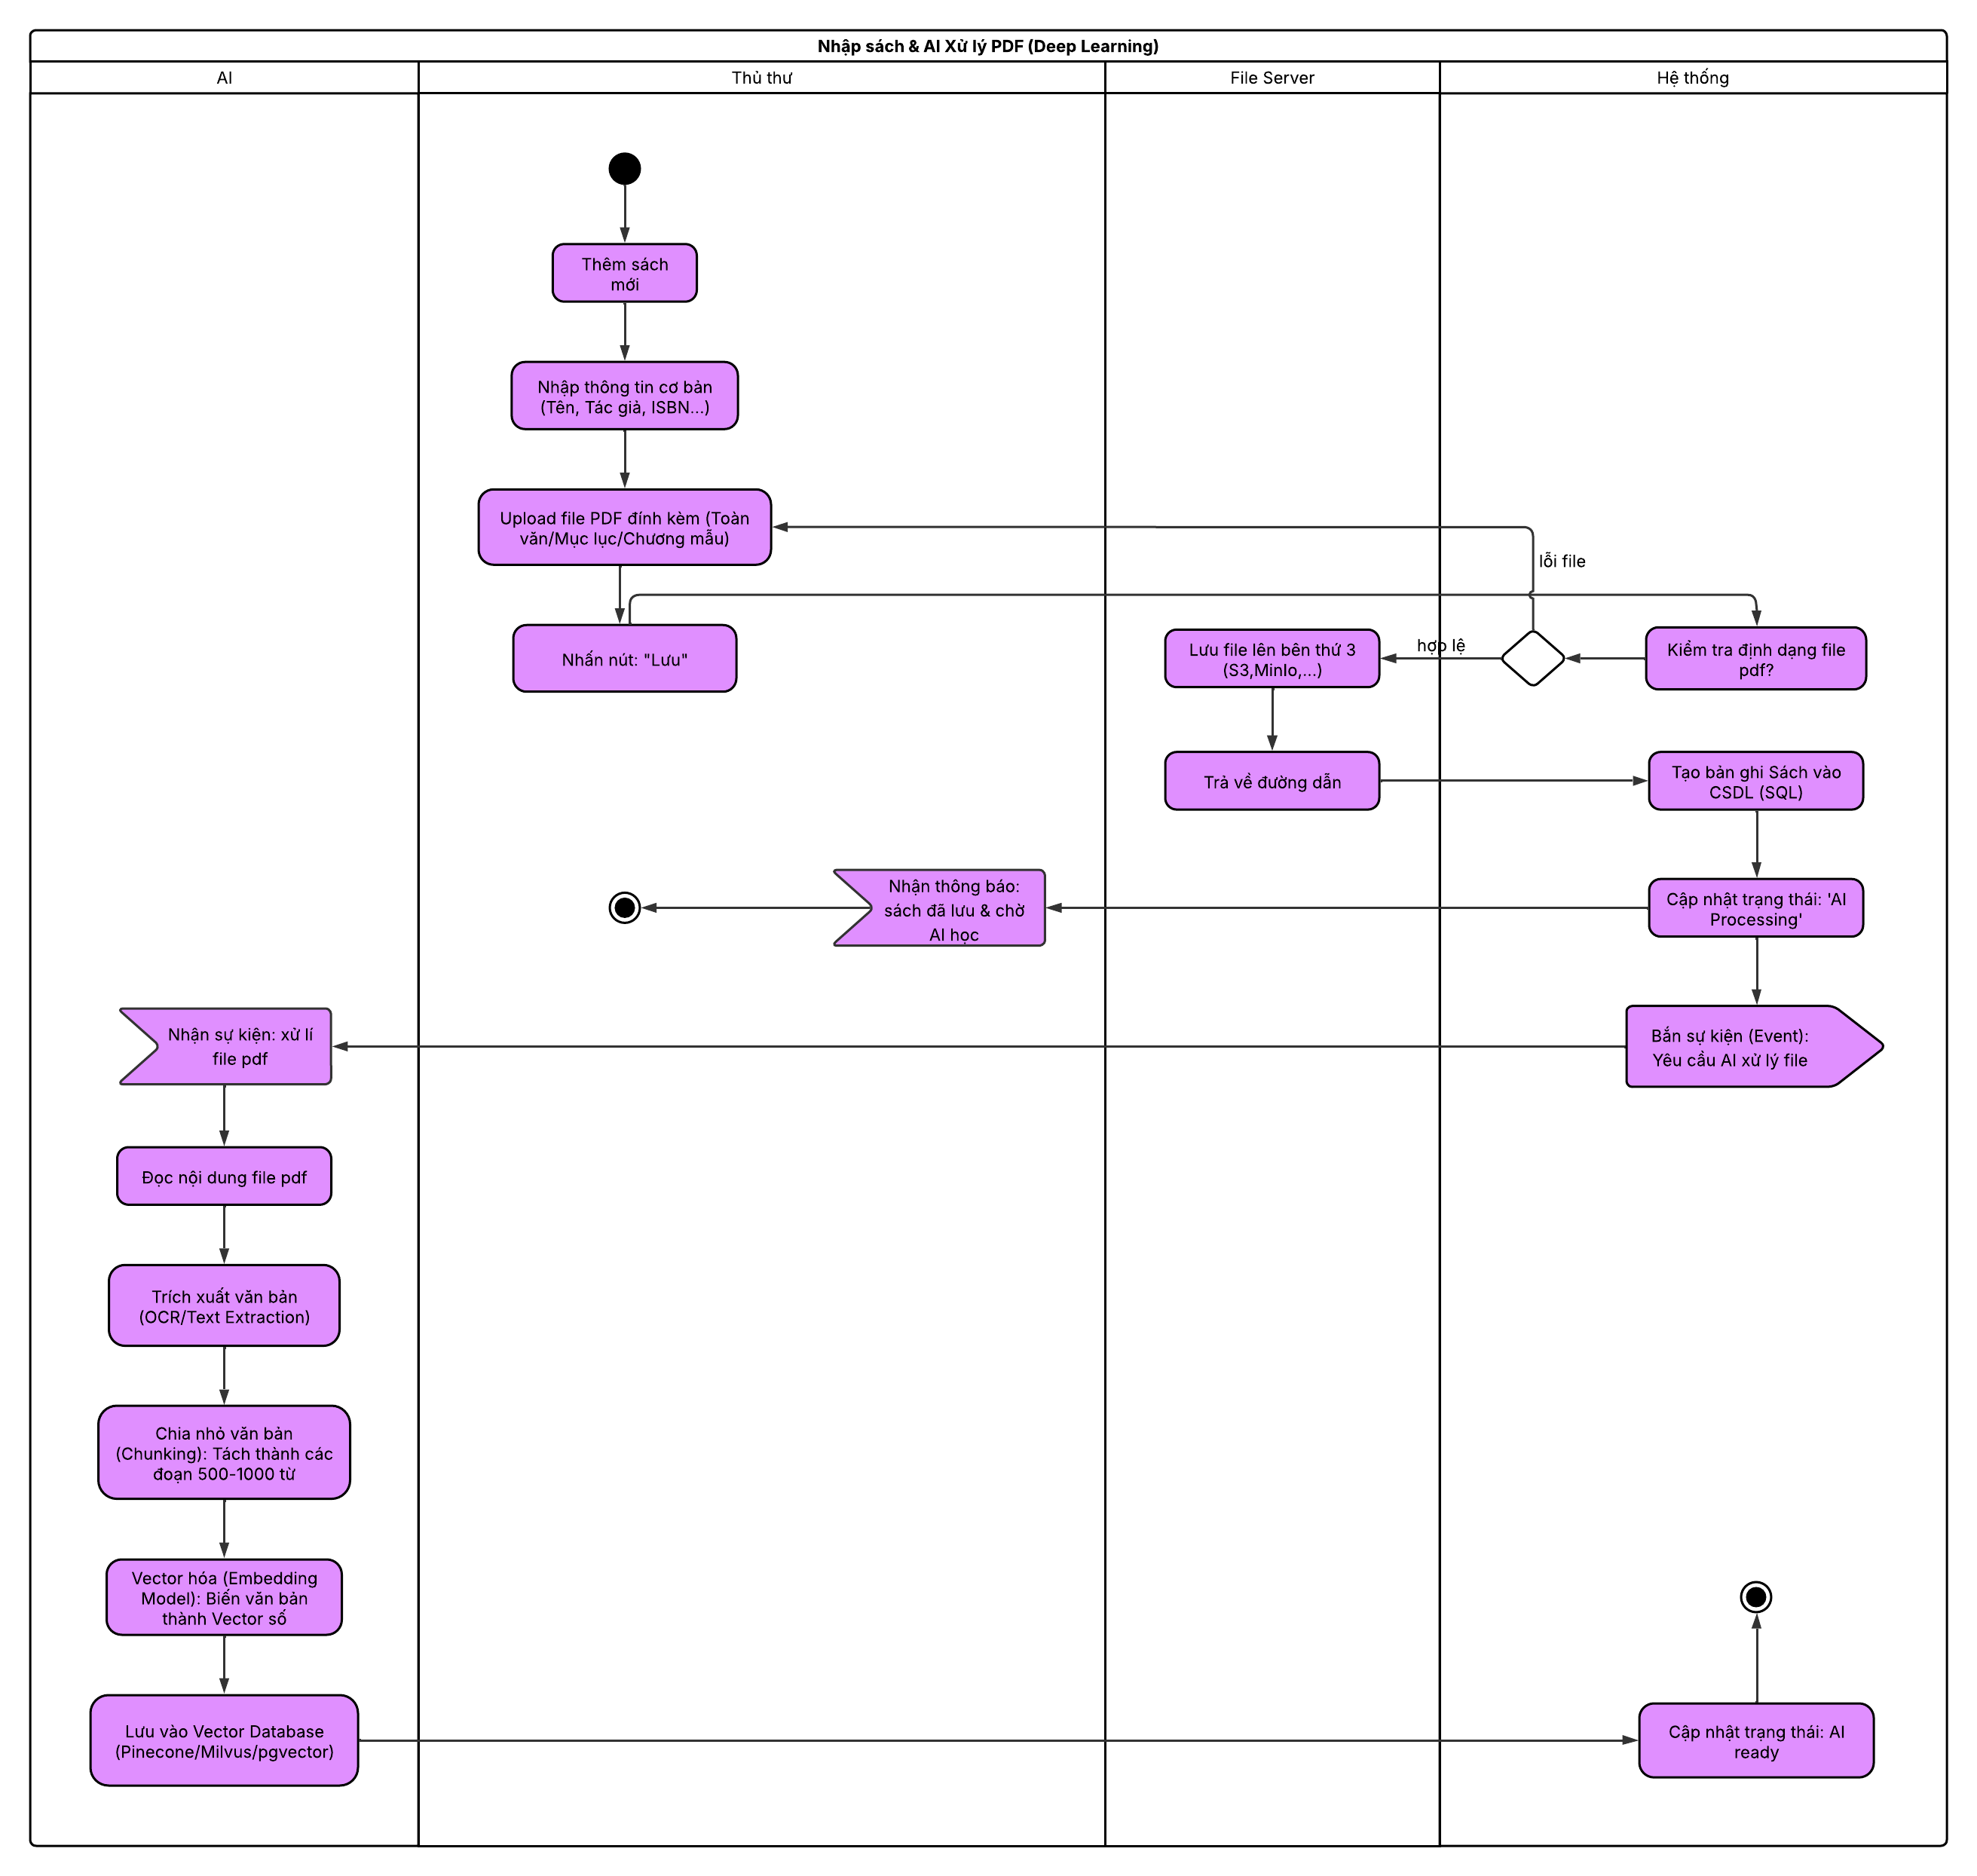
\includegraphics[width=\linewidth]{figures/ch05/activity/add_book.png}
 \caption{Tạo sách với AI — Activity Diagram}
 \label{fig:create_book}
\end{figure}

\FloatBarrier

\section{Giải pháp công nghệ}
\label{sec:giai_phap_cong_nghe}

Việc lựa chọn công nghệ không chỉ dựa trên mức độ phổ biến của framework, mà dựa trên mức độ phù hợp với bài toán thư viện đã hiện thực. Nhóm sử dụng năm tiêu chí chính: \textbf{hiệu năng và độ trễ}, \textbf{khả năng bảo trì}, \textbf{bảo mật và phân quyền}, \textbf{trải nghiệm phát triển}, và \textbf{chi phí triển khai trong phạm vi đồ án}. Từ các tiêu chí này, hệ thống được chia thành ba phần rõ ràng: frontend phục vụ trải nghiệm người dùng, backend giữ nghiệp vụ và dữ liệu giao dịch, còn AI service xử lý các workload tính toán nặng.

\subsection{Front-end}
\label{subsec:frontend_solution}

Frontend của hệ thống là một \textbf{single-page application} phục vụ cả trang public, khu vực bạn đọc và dashboard thủ thư. Đặc điểm chính của phần này là nhiều form nghiệp vụ, nhiều màn hình trạng thái, gọi REST API liên tục, nhận thông báo realtime và upload file PDF trực tiếp lên S3-compatible storage bằng presigned URL. Vì vậy, công nghệ frontend cần nhẹ khi triển khai, dễ chia component và đủ linh hoạt để bám sát thiết kế Figma.

Nhóm đã so sánh các lựa chọn phổ biến theo đúng bối cảnh này:

\begin{table}[H]
\centering
\small
\renewcommand{\arraystretch}{1.12}
\setlength{\tabcolsep}{5pt}
\begin{tabularx}{\linewidth}{|>{\bfseries}l|>{\raggedright\arraybackslash}X|%
>{\raggedright\arraybackslash}X|%
>{\raggedright\arraybackslash}X|}
\hline
\textbf{Nền tảng} & \textbf{Ưu điểm} & \textbf{Nhược điểm} & \textbf{Kết luận} \\
\hline
\textbf{React + Vite} & Phù hợp với SPA nhiều tương tác; build gọn; HMR nhanh; triển khai như static assets; dễ tích hợp REST API, WebSocket/STOMP và presigned upload. Hệ sinh thái React đáp ứng tốt dashboard, form nghiệp vụ và component tái sử dụng. & Không có SSR mặc định; SEO cho public pages không mạnh bằng framework SSR; nhóm phải tự chuẩn hóa routing, state, API layer và cấu trúc component. & \textbf{Được chọn}. Hệ thống chủ yếu là ứng dụng nghiệp vụ sau đăng nhập, không cần SSR phức tạp. React/Vite giúp triển khai đơn giản qua NGINX/Docker, giảm nhu cầu Node runtime và vẫn đủ linh hoạt cho public pages, reader pages và librarian dashboard. \\
\hline
Next.js & Mạnh về SSR/SSG, SEO, route-level data fetching và tối ưu website public lớn. Phù hợp khi nội dung cần index mạnh hoặc cần render phía server. & Cần Node.js runtime, tăng thêm lớp vận hành. Nếu dùng cho hệ thống này, một phần trách nhiệm trình bày và xác thực dễ bị chồng lên Spring Boot API. & Không chọn vì bài toán chính là dashboard và nghiệp vụ thư viện, không phải website nội dung cần SEO mạnh. Lợi ích SSR không đủ bù cho chi phí vận hành thêm. \\
\hline
Nuxt (Vue) & Có SSR/SSG tốt trong hệ sinh thái Vue, cú pháp dễ tiếp cận và tổ chức project rõ ràng. & Không cùng hệ sinh thái với phần frontend đã xây dựng; chuyển sang Vue/Nuxt làm tăng chi phí học lại component, router, test và thư viện UI. & Không chọn vì nhóm đã hiện thực ổn định bằng React và cần tận dụng các thư viện React cho icon, form, realtime notification và dashboard. \\
\hline
Angular & Framework đầy đủ, opinionated, mạnh về form, dependency injection, routing và cấu trúc enterprise. & Boilerplate nhiều, đường cong học tập cao, nặng hơn nhu cầu của nhóm. Việc tùy biến UI nhanh theo Figma kém linh hoạt hơn React trong phạm vi đồ án. & Không chọn vì hệ thống cần tốc độ phát triển và khả năng tinh chỉnh giao diện cao hơn là một framework enterprise lớn ngay từ đầu. \\
\hline
\end{tabularx}
\caption{So sánh công nghệ Front-end theo tiêu chí của hệ thống}
\label{tab:frontend-compare}
\end{table}
\FloatBarrier

\textbf{Lựa chọn:} \emph{React + Vite kết hợp với TypeScript, Tailwind CSS, React Router DOM với HashRouter, Axios, lucide-react, sonner, SockJS/STOMP và một bộ component tự xây dựng theo thiết kế Figma.}

\subsubsection*{Lý do chọn theo tiêu chí chuyên môn}

\begin{itemize}
    \item \textbf{Tốc độ phát triển vượt trội (Developer Experience):}
    Vite tận dụng cơ chế native ES modules trong môi trường phát triển và dùng esbuild cho nhiều bước tiền xử lý, nhờ đó thời gian khởi động dev server và Hot Module Replacement nhanh hơn đáng kể so với cấu hình Webpack truyền thống. Với một frontend có nhiều trang nghiệp vụ, điều này giúp nhóm lặp nhanh khi chỉnh giao diện, form và luồng tương tác.

    \item \textbf{Triển khai đơn giản qua NGINX:}
    React + Vite tạo ra các file tĩnh (HTML/CSS/JS) sau khi build, có thể phục vụ trực tiếp bởi NGINX mà không cần Node.js server runtime. Điều này giúp giảm tài nguyên máy chủ, đơn giản hóa cấu hình Docker và tận dụng khả năng cache tĩnh của NGINX để tăng hiệu năng.

    \item \textbf{Phù hợp với đặc thù hệ thống:}
    Phần lớn giao diện của hệ thống là các trang dashboard và luồng nghiệp vụ dành cho người dùng đã đăng nhập, ví dụ quản lý mượn--trả, đặt trước, phí phạt, thông báo và upload tài liệu. Những trang này ưu tiên tốc độ tương tác và tính ổn định hơn SEO. Bảo mật API được đảm bảo ở Backend Spring Boot bằng JWT và kiểm tra vai trò, nên không cần thêm một lớp server-side rendering trung gian.

    \item \textbf{Hệ sinh thái React và tính nhất quán giao diện:}
    \textbf{TypeScript} giúp giảm lỗi khi tích hợp với API backend, trong khi \textbf{Tailwind CSS}, \textbf{lucide-react}, \textbf{sonner}, \textbf{react-select} và các component tự xây dựng giúp nhóm kiểm soát tốt giao diện mà không phụ thuộc nặng vào một UI framework lớn. Cách làm này phù hợp với hệ thống có nhiều màn hình nghiệp vụ cần tinh chỉnh riêng cho bạn đọc và thủ thư.

    \item \textbf{Quản lý trạng thái và Routing:}
    \textbf{React Router DOM} với \textbf{HashRouter} được dùng để tổ chức các nhóm trang public, reader và librarian, phù hợp với kiểu deploy static qua NGINX. Các trạng thái dùng chung như xác thực, ngôn ngữ, theme, thông báo realtime và upload file được quản lý bằng React Context; các lời gọi API được gom qua Axios service để thống nhất xử lý token, lỗi và phản hồi từ backend.
\end{itemize}

\FloatBarrier

\subsection{Back-end}
\label{subsec:backend_solution}

Backend là phần lõi của hệ thống vì chịu trách nhiệm xác thực, phân quyền, quản lý dữ liệu thư viện và đảm bảo tính nhất quán cho các giao dịch mượn--trả. Khác với frontend, backend không chỉ cần tạo API nhanh mà còn phải xử lý transaction, khóa bản sao khi mượn/trả, phí phạt, đặt trước, webhook thanh toán và callback từ AI service. Vì vậy tiêu chí ưu tiên là độ tin cậy, transaction ACID, bảo mật và khả năng tổ chức module rõ ràng.

\begin{table}[H]
\centering
\small
\renewcommand{\arraystretch}{1.12}
\setlength{\tabcolsep}{5pt}
\begin{tabularx}{\linewidth}{|>{\bfseries}l|>{\raggedright\arraybackslash}X|%
>{\raggedright\arraybackslash}X|%
>{\raggedright\arraybackslash}X|}
 \hline
 \textbf{Nền tảng}
& \textbf{Ưu điểm}
& \textbf{Nhược điểm}
& \textbf{Quyết định} \\
 \hline
 \textbf{Spring Boot}
& Mạnh về nghiệp vụ giao dịch, Spring Security, transaction ACID, JPA/JDBC, validation, scheduler, Kafka/WebSocket và tích hợp dịch vụ ngoài. Phù hợp với mô hình dữ liệu quan hệ chặt chẽ của thư viện.
& Verbose hơn Node/Python; cần thiết kế module rõ ràng để tránh monolith bị rối khi số use case tăng.
& \textbf{Được chọn}. Lõi hệ thống có nhiều nghiệp vụ cần tính nhất quán: mượn--trả, đặt trước, phí phạt, bản sao, thanh toán và phân quyền. Spring Boot giúp kiểm soát transaction, bảo mật và ranh giới module tốt hơn trong bối cảnh hiện thực hiện tại. \\
 \hline
NestJS / Express
& Phát triển API nhanh, TypeScript đồng bộ với frontend, hệ sinh thái lớn và dễ tuyển dụng.
& Express quá tự do nên cần tự chuẩn hóa nhiều thứ; NestJS tốt hơn nhưng transaction, JPA-style domain modeling và security enterprise không tự nhiên bằng Spring Boot trong bài toán này.
& Không được chọn vì lợi thế dùng chung ngôn ngữ không đủ bù cho yêu cầu transaction và phân quyền chặt chẽ của nghiệp vụ thư viện. \\
 \hline
Django / DRF
& CRUD nhanh, admin mạnh, Python thuận lợi nếu gộp chung backend với AI.
& Nếu gộp nghiệp vụ và AI vào một codebase Python, ranh giới giữa transaction nghiệp vụ và workload AI dễ bị lẫn. Khả năng module hóa theo DDD/Clean Architecture trong dự án hiện tại không thuận lợi bằng Spring Boot.
& Không được chọn cho core backend; Python được giữ đúng vai trò ở AI service, nơi hệ sinh thái ML phát huy giá trị nhất. \\
 \hline
MongoDB (NoSQL)
& Schema linh hoạt, dễ lưu tài liệu JSON và mở rộng ngang trong một số bài toán dữ liệu phi cấu trúc.
& Không phù hợp làm datastore chính cho quan hệ nhiều chiều giữa ấn phẩm, bản sao, giao dịch mượn, phí phạt, đặt trước và người dùng. Join, constraint và transaction liên bảng là yêu cầu cốt lõi của hệ thống.
& Không được chọn vì PostgreSQL đáp ứng tốt hơn cả dữ liệu quan hệ lẫn dữ liệu AI nhờ JSONB và pgvector. \\
 \hline
\end{tabularx}
\caption{So sánh công nghệ Back-end theo tiêu chí của hệ thống}
\label{tab:backend-compare}
\end{table}
\FloatBarrier

\textbf{Lựa chọn:} \emph{Spring Boot 3.3, Java 21, Spring Security với JWT/OAuth2, Spring Data JPA kết hợp JDBC Template cho truy vấn đặc thù, PostgreSQL, Flyway, Kafka, WebSocket/STOMP, S3-compatible storage, PayOS và OpenAPI/Swagger. Mô-đun AI/NLP được tách thành một service riêng sử dụng Python/FastAPI.}

\subsubsection*{Lý do chọn theo tiêu chí chuyên môn}
\begin{itemize}
 \item \textbf{Độ tin cậy và Hiệu năng:} Spring Boot là một framework đã được kiểm chứng về độ ổn định và hiệu năng trong các hệ thống enterprise. Kết hợp với \textbf{Java Virtual Machine (JVM)}, nó cung cấp khả năng xử lý đồng thời mạnh mẽ, phù hợp với các tác vụ CRUD và giao dịch phức tạp. Các truy vấn catalog được phân trang và tối ưu bằng PostgreSQL; các tác vụ phụ như email, thông báo và một số xử lý nền được tách khỏi luồng chính bằng Kafka, WebSocket và executor bất đồng bộ.

 \item \textbf{Mô hình Dữ liệu và Khả năng mở rộng:} Nghiệp vụ thư viện có bản chất là quan hệ chặt chẽ. \textbf{Spring Data JPA} và \textbf{Hibernate} cung cấp một tầng ORM (Object-Relational Mapping) mạnh mẽ, cho phép mô hình hóa các thực thể và mối quan hệ phức tạp một cách tự nhiên. Việc sử dụng \textbf{Specification Pattern} giúp xây dựng các truy vấn động một cách an toàn và dễ bảo trì, phục vụ cho các yêu cầu lọc và tìm kiếm phức tạp.

 \item \textbf{Bảo mật Toàn diện:} \textbf{Spring Security} cho phép triển khai xác thực và phân quyền theo vai trò một cách rõ ràng. Hệ thống sử dụng \textbf{JWT} với access token và refresh token cho kiến trúc stateless API; backend chịu trách nhiệm kiểm tra quyền truy cập ở các endpoint quản trị, endpoint mượn--trả, thanh toán và callback từ AI service. Các luồng nhạy cảm như upload file và webhook thanh toán được đặt sau các cơ chế xác thực hoặc chữ ký tương ứng.

 \item \textbf{Ranh giới module rõ ràng:} Backend được tổ chức thành các module Maven như auth, user, catalog, circulation, recommendation và shared. Cách chia này giữ được ưu điểm triển khai đơn giản của modular monolith, nhưng vẫn tạo ranh giới nghiệp vụ đủ rõ để kiểm thử, bảo trì và tách service trong tương lai nếu cần.

 \item \textbf{Dịch vụ AI độc lập:} Việc tách mô-đun AI/NLP thành một service riêng bằng Python/FastAPI là một quyết định kiến trúc có chủ đích. Backend Java giữ phần transaction, phân quyền và nghiệp vụ; AI service giữ phần embedding, semantic search, Gemini reduce và recommendation. Cách chia này tránh nhồi ML workload vào core backend, nhưng vẫn đơn giản hơn việc tách toàn bộ hệ thống thành microservices.
\end{itemize}

\FloatBarrier

\subsection*{Kết luận về Sự phối hợp giữa hai nền tảng}
Kiến trúc tổng thể được thiết kế theo mô hình \textbf{frontend tĩnh + backend API + AI service}. \textbf{React/Vite SPA} chịu trách nhiệm trải nghiệm người dùng và gọi REST API; \textbf{Spring Boot API} giữ vai trò lõi nghiệp vụ, xác thực, phân quyền và điều phối dữ liệu; \textbf{FastAPI AI Service} xử lý các tác vụ nặng như embedding, semantic search và recommendation. Sự phân tách này đủ rõ để bảo trì, nhưng vẫn giữ chi phí triển khai thấp hơn so với một kiến trúc microservices đầy đủ.




\section{Ứng dụng AI vào hệ thống}
% =========================================================================================
Trong hệ thống LMS, AI không được đặt vào như một chức năng phụ để ``làm đẹp'' sản phẩm. AI được thiết kế như một \textbf{lớp năng lực hỗ trợ khám phá tri thức}: đọc nội dung PDF, hiểu ý định tìm kiếm của bạn đọc và đề xuất tài liệu phù hợp với hành vi sử dụng thật.

Điểm quan trọng nhất trong thiết kế là \textbf{AI không thay thế nghiệp vụ thư viện}. Các nghiệp vụ như mượn--trả, đặt trước, quản lý bản sao, phí phạt, thanh toán và phân quyền vẫn do backend Spring Boot kiểm soát. AI Service chỉ xử lý các bài toán phù hợp với ML/NLP, sau đó trả về \textbf{metadata bổ trợ}, \textbf{danh sách \texttt{publication\_id}} hoặc \textbf{chiến lược gợi ý}; backend luôn là nơi lấy dữ liệu cuối cùng trước khi trả về frontend.

\begin{itemize}
    \item \textbf{Module 1 -- Xử lý PDF file:} biến file PDF do thủ thư upload thành dữ liệu có thể tìm kiếm và gợi ý.
    \item \textbf{Module 2 -- Hỗ trợ tìm kiếm ngữ nghĩa:} giúp bạn đọc tìm theo ý định, không chỉ theo từ khóa chính xác.
    \item \textbf{Module 3 -- Gợi ý cá nhân hoá:} kết hợp nội dung sách, hành vi người dùng và fallback nghiệp vụ để đề xuất sách có thể mượn.
\end{itemize}

Nhóm chọn mô hình \textbf{AI Satellite Service}: backend Java giữ nghiệp vụ và giao dịch; AI Service Python/FastAPI xử lý workload nặng như đọc PDF, sinh embedding, truy vấn pgvector và recommendation. Cách tách này giúp hệ thống vừa \textbf{giữ lõi nghiệp vụ ổn định}, vừa \textbf{tận dụng hệ sinh thái AI của Python}.

\begin{figure}[H]
\centering
\begin{tikzpicture}[
    % Sử dụng positioning giúp quản lý khoảng cách các khối linh hoạt và rộng rãi hơn
    node distance=1.5cm and 2.5cm,
    every node/.style={font=\small\sffamily},
    box/.style={rectangle, draw=blue!65!black, fill=blue!5, thick, rounded corners=3pt, minimum width=3.5cm, minimum height=1.2cm, align=center},
    ai/.style={rectangle, draw=green!55!black, fill=green!6, thick, rounded corners=3pt, minimum width=3.5cm, minimum height=1.2cm, align=center},
    db/.style={cylinder, draw=orange!80!black, fill=orange!7, shape border rotate=90, aspect=0.22, minimum width=2.5cm, minimum height=1.5cm, align=center},
    arrow/.style={thick, ->, >=stealth},
    label text/.style={font=\small, midway}
]
    % --- Định nghĩa các khối hệ thống (Nodes) ---
    \node[box] (fe) {Frontend\\React/Vite};
    \node[box, right=of fe] (be) {Backend\\Spring Boot};
    \node[ai, right=of be] (ai) {AI Service\\FastAPI};

    \node[db, below=of be] (pg) {PostgreSQL\\Catalog};
    \node[db, below=of ai] (vec) {pgvector\\AI schema};

    % --- Định nghĩa đường nối luồng dữ liệu (Arrows) ---
    \draw[arrow] (fe) -- node[label text, above] {REST API} (be);
    \draw[arrow] (be) -- node[label text, above] {AI Gateway} (ai);
    \draw[arrow] (be) -- node[label text, left] {nghiệp vụ} (pg);
    \draw[arrow] (ai) -- node[label text, right] {vectors / ETL / cache} (vec);
    \draw[arrow] (vec) -- node[label text, above] {publication ids} (pg);
\end{tikzpicture}
\caption{Trách nhiệm giữa frontend, backend và AI service}
\label{fig:ai_integration_boundary}
\end{figure}

\begin{table}[H]
\centering
\small
\renewcommand{\arraystretch}{1.18}
\setlength{\tabcolsep}{5pt}
\begin{tabularx}{\linewidth}{|>{\bfseries}p{0.23\linewidth}|>{\raggedright\arraybackslash}X|>{\raggedright\arraybackslash}X|}
\hline
\textbf{Thành phần} & \textbf{Trách nhiệm chính} & \textbf{Điểm nhấn thiết kế} \\
\hline
Frontend & Upload tài liệu, gửi truy vấn, hiển thị trạng thái AI và kết quả đã chuẩn hóa. & \textbf{Không gọi trực tiếp model AI}; mọi request đi qua backend. \\
\hline
Backend & Xác thực, phân quyền, lưu catalog, quản lý bản sao/giao dịch và lấy metadata cuối cùng. & \textbf{Là nguồn sự thật nghiệp vụ}; AI không được quyết định trạng thái mượn--trả. \\
\hline
AI Service & Xử lý PDF, sinh embedding, tìm kiếm ngữ nghĩa, tạo metadata AI và recommendation. & \textbf{Chỉ trả kết quả suy luận}; backend quyết định dữ liệu hiển thị cuối cùng. \\
\hline
\end{tabularx}
\caption{Ranh giới trách nhiệm khi tích hợp AI}
\label{tab:ai_responsibility_boundary}
\end{table}

\subsection{Cơ sở thiết kế dữ liệu AI}

Trước khi hiện thực, nhóm xác định rõ AI cần ba nhóm dữ liệu đầu vào. Cách
thiết kế này giúp tránh tình trạng ``có model trước rồi mới tìm dữ liệu'', đồng
thời bảo đảm mỗi thuật toán đều có nguồn tín hiệu khả thi trong hệ thống thư
viện.

\begin{table}[H]
\centering
\small
\renewcommand{\arraystretch}{1.18}
\setlength{\tabcolsep}{4pt}
\begin{tabularx}{\linewidth}{|>{\bfseries}p{0.2\linewidth}|>{\raggedright\arraybackslash}X|>{\raggedright\arraybackslash}X|}
\hline
\textbf{Nhóm dữ liệu} & \textbf{Nguồn trong hệ thống} & \textbf{Dùng cho bài toán AI} \\
\hline
Nội dung tài liệu & PDF, tiêu đề, phụ đề, mô tả, mục lục, tác giả, danh mục, tag. & Embedding, semantic search, sách tương tự, content-based recommendation. \\
\hline
Hành vi người dùng & Lượt xem, wishlist, mượn sách, rating, lịch sử tìm kiếm. & Collaborative filtering, ALS implicit feedback, trending fallback. \\
\hline
Trạng thái nghiệp vụ & Sách còn bản sao hay không, chi nhánh, trạng thái bản sao, quyền truy cập. & Lọc kết quả cuối cùng để gợi ý/tìm kiếm có giá trị sử dụng thật. \\
\hline
\end{tabularx}
\caption{Nguồn dữ liệu dùng cho thiết kế AI}
\label{tab:ai_data_sources_design}
\end{table}

Về mặt lưu trữ, nhóm chọn hướng \textbf{vector theo chunk} thay vì một vector
duy nhất cho cả sách. Một sách có thể bao gồm nhiều chủ đề; nếu chỉ dùng một
vector trung bình cho toàn bộ tài liệu, các chương nhỏ nhưng quan trọng dễ bị
loãng. Vì vậy, mỗi chunk có một embedding riêng và liên kết về
\texttt{publication\_id}.

\begin{lstlisting}[language=SQL, caption={Thiết kế bảng vector phục vụ semantic search}, label={lst:ai_vector_schema_design}]
CREATE TABLE ai_engine.publication_vectors (
    id BIGSERIAL PRIMARY KEY,
    publication_id BIGINT NOT NULL,
    chunk_index INT NOT NULL,
    chunk_text TEXT NOT NULL,
    embedding VECTOR(768) NOT NULL,
    created_at TIMESTAMP DEFAULT NOW()
);

CREATE INDEX idx_publication_vectors_embedding
ON ai_engine.publication_vectors
USING hnsw (embedding vector_cosine_ops);
\end{lstlisting}

\FloatBarrier

\subsection{Module 1: Xử lý PDF file}

\textbf{Mục tiêu của module này} là biến một file PDF thô thành dữ liệu có giá trị cho hệ thống: \textbf{summary}, \textbf{audience}, \textbf{tag}, \textbf{vector embedding} và \textbf{trạng thái xử lý AI}. Đây là module nền tảng: nếu PDF không được xử lý tốt, semantic search và recommendation phía sau sẽ không có đủ dữ liệu để hoạt động.

Luồng xử lý được thiết kế theo hướng \textbf{không chặn thao tác của thủ thư}. Thủ thư chỉ cần upload tài liệu; backend lưu URL tài liệu và kích hoạt AI xử lý ở phía sau.

\begin{figure}[H]
\centering
\resizebox{\linewidth}{!}{%
\begin{tikzpicture}[
    every node/.style={font=\small},
    flowstep/.style={rectangle, draw=blue!70!black, fill=blue!5, thick, rounded corners, minimum width=3.05cm, minimum height=1.0cm, align=center},
    store/.style={cylinder, draw=orange!80!black, fill=orange!8, shape border rotate=90, aspect=0.25, minimum width=2.3cm, minimum height=1.35cm, align=center},
    resultnode/.style={rectangle, draw=green!55!black, fill=green!6, thick, rounded corners, minimum width=3.2cm, minimum height=1.0cm, align=center},
    arrow/.style={thick, ->, >=stealth}
]
    \node[flowstep] (fe) at (0,0) {1. Thủ thư\\chọn PDF};
    \node[flowstep] (url) at (3.8,0) {2. Backend cấp\\upload URL};
    \node[store] (s3) at (7.2,0) {Object\\Storage};
    \node[flowstep] (save) at (10.8,0) {3. Lưu\\\texttt{file\_url}};
    \node[resultnode] (ai) at (10.8,-2.0) {4. Gọi AI\\process PDF};
    \node[resultnode] (etl) at (7.2,-2.0) {5. Clean\\chunk\\embed};
    \node[resultnode] (meta) at (3.8,-2.0) {6. Gemini\\reduce metadata};
    \node[store] (db) at (0,-2.0) {DB\\AI outputs};

    \draw[arrow] (fe) -- (url);
    \draw[arrow] (url) -- (s3);
    \draw[arrow] (s3) -- (save);
    \draw[arrow] (save) -- (ai);
    \draw[arrow] (ai) -- (etl);
    \draw[arrow] (etl) -- (meta);
    \draw[arrow] (meta) -- (db);
\end{tikzpicture}
}
\caption{Module 1 -- Luồng xử lý PDF file sau khi thủ thư upload}
\label{fig:ai_pdf_processing_flow}
\end{figure}

\begin{table}[H]
\centering
\small
\renewcommand{\arraystretch}{1.15}
\setlength{\tabcolsep}{4pt}
\begin{tabularx}{\linewidth}{|>{\bfseries}p{0.22\linewidth}|>{\raggedright\arraybackslash}X|>{\raggedright\arraybackslash}X|}
\hline
\textbf{Giai đoạn} & \textbf{Thiết kế} & \textbf{Điểm nhấn báo cáo} \\
\hline
Upload và lưu file & Frontend xin \textbf{presigned upload URL}; file PDF được đẩy lên object storage; backend lưu lại \texttt{file\_url}/\texttt{s3Key} cho publication. & \textbf{File được lưu trước, AI xử lý sau}; thao tác tạo/cập nhật sách không bị khóa bởi pipeline AI. \\
\hline
ETL nội dung & AI Service dùng \textbf{PyMuPDF} để trích xuất text, làm sạch header/footer/số trang, sau đó chia chunk bằng sliding window. & \textbf{Index nội dung thật của PDF}, không chỉ index tiêu đề hay mô tả thủ công. \\
\hline
Embedding và metadata & Chunk được vector hóa và lưu vào \texttt{ai\_engine.publication\_vectors}; Gemini chỉ được gọi ở bước reduce để tạo summary, audience và tag. & \textbf{Không gọi LLM trong mỗi lần tìm kiếm}; giảm độ trễ, giảm quota và tăng độ ổn định. \\
\hline
Theo dõi trạng thái & Kết quả xử lý được lưu với trạng thái \texttt{RUNNING}, \texttt{SUCCESS}, \texttt{FAILED}; nếu lỗi, catalog vẫn giữ ấn phẩm. & \textbf{AI lỗi không làm hỏng nghiệp vụ thư viện}. \\
\hline
\end{tabularx}
\caption{Thiết kế Module 1 -- Xử lý PDF file}
\label{tab:ai_module_pdf}
\end{table}

\subsubsection{Thiết kế chunking, embedding và reduce metadata}

PDF không được đưa thẳng vào LLM. Nhóm thiết kế pipeline theo hướng
\textbf{extract trước, chunk sau, embedding độc lập, LLM chỉ reduce}. Cách này
giảm chi phí gọi LLM và làm cho semantic search có thể chạy hoàn toàn trên
vector đã tính sẵn.

\begin{table}[H]
\centering
\small
\renewcommand{\arraystretch}{1.18}
\begin{tabularx}{\linewidth}{|>{\bfseries}p{0.22\linewidth}|>{\raggedright\arraybackslash}X|>{\raggedright\arraybackslash}X|}
\hline
\textbf{Bước} & \textbf{Thiết kế trước hiện thực} & \textbf{Lý do} \\
\hline
Làm sạch PDF & Bỏ header/footer lặp, số trang, ký tự null, khoảng trắng nhiễu và từ bị ngắt dòng. & Vector phải biểu diễn nội dung thật, không học nhiễu trình bày. \\
\hline
Sliding window chunk & Chia text thành các đoạn độ dài $L$, overlap $O$, bước nhảy $S=L-O$. & Giữ ngữ cảnh giữa hai chunk liền kề, tránh cắt mất câu/ý. \\
\hline
Normalize embedding & Với chunk $c_i$, tính $e_i=\frac{f(c_i)}{\|f(c_i)\|_2}$. & Vector đã chuẩn hóa giúp cosine similarity ổn định. \\
\hline
Chọn chunk đại diện & Ưu tiên chunk mở đầu, chunk gần centroid và chunk đa dạng theo MMR. & Reduce metadata cần đại diện toàn tài liệu, không chỉ vài đoạn gần nhau. \\
\hline
\end{tabularx}
\caption{Thiết kế xử lý PDF trước khi gọi LLM}
\label{tab:ai_pdf_algorithm_design}
\end{table}

Với tập vector chunk $E=\{e_1,e_2,\ldots,e_n\}$, vector trung tâm của tài liệu
được tính:

\[
\bar{e}=\frac{1}{n}\sum_{i=1}^{n} e_i
\]

Khi chọn thêm chunk đại diện, nhóm dùng ý tưởng Maximal Marginal Relevance
(MMR): cân bằng giữa độ liên quan với tài liệu và độ đa dạng so với các chunk đã
chọn.

\[
\mathrm{MMR}(c_i)=\lambda \cdot \mathrm{sim}(e_i,\bar{e}) -
(1-\lambda)\cdot \max_{c_j \in S}\mathrm{sim}(e_i,e_j)
\]

Trong đó $S$ là tập chunk đã chọn. Thiết kế này phù hợp với báo cáo đồ án vì nó
cho thấy metadata sinh ra không phụ thuộc mù quáng vào toàn bộ PDF dài, mà được
tạo từ các đoạn đại diện có kiểm soát.

\subsubsection{Thiết kế prompt LLM và lựa chọn model}

LLM chỉ được dùng cho bài toán \textbf{reduce metadata học thuật}, không dùng để
quyết định kết quả tìm kiếm hay gợi ý. Nhóm chọn cấu hình mặc định
\textbf{\texttt{gemini-2.5-flash-lite}} cho bước này vì ba lý do: tốc độ phản
hồi phù hợp với pipeline nền, chi phí thấp hơn các model lớn, và đủ năng lực để
tổng hợp summary/tag từ các excerpt đã được chọn lọc. Nếu cần tăng chất lượng
trong các lần xử lý lại dữ liệu, thiết kế vẫn cho phép cấu hình thêm một model
premium làm phương án thử lại; tuy nhiên pipeline chính không phụ thuộc vào
model đắt tiền.

\begin{table}[H]
\centering
\small
\renewcommand{\arraystretch}{1.18}
\begin{tabularx}{\linewidth}{|>{\bfseries}p{0.24\linewidth}|>{\raggedright\arraybackslash}X|}
\hline
\textbf{Quyết định} & \textbf{Thiết kế} \\
\hline
Model LLM & \texttt{gemini-2.5-flash-lite} cho reduce metadata; model premium chỉ là cấu hình tùy chọn khi cần retry/chất lượng cao hơn. \\
\hline
Model embedding & \texttt{bkai-foundation-models/vietnamese-bi-encoder}, phù hợp văn bản tiếng Việt và sinh vector dùng cho semantic search. \\
\hline
Dữ liệu đưa vào LLM & Chỉ đưa \texttt{CONTENT\_EXCERPTS} đã chọn bằng MMR và \texttt{CATALOG\_CONTEXT} ngắn để khử nhập nhằng. \\
\hline
Dữ liệu đầu ra & Một JSON duy nhất gồm \texttt{master\_summary}, \texttt{audience}, \texttt{tags}, \texttt{tags\_en}. \\
\hline
Nguyên tắc an toàn & Không cho LLM bịa theo title/author/category; không cho trả markdown; validate JSON và fallback deterministic nếu lỗi. \\
\hline
\end{tabularx}
\caption{Thiết kế sử dụng LLM trong pipeline AI}
\label{tab:ai_llm_model_prompt_design}
\end{table}

Prompt được thiết kế theo hướng \textbf{ràng buộc đầu ra trước, nội dung đầu vào
sau}. Điều này làm giảm rủi ro LLM trả lời dài dòng hoặc tạo metadata không thể
lưu vào hệ thống.

\begin{lstlisting}[caption={Khung prompt reduce metadata cho LLM}, label={lst:ai_llm_prompt_design}]
ROLE:
  University librarian and academic cataloging specialist.

TASK:
  Read CONTENT_EXCERPTS from a PDF and create library metadata.

RULES:
  1. master_summary must be based only on CONTENT_EXCERPTS.
  2. CATALOG_CONTEXT is only for disambiguation, not summary generation.
  3. Do not describe AI, metadata, library workflow, or the PDF file itself.
  4. Tags must be specific topics/skills/technologies, not title or author.
  5. Ignore OCR/PDF noise: page numbers, headers, footers, copyright.
  6. tags_en must align 1-1 with tags and use standard English terms.

OUTPUT JSON ONLY:
{
  "master_summary": "120-180 Vietnamese words, 4-6 sentences",
  "audience": "one valid faculty code",
  "tags": ["exactly 5 Vietnamese tags"],
  "tags_en": ["exactly 5 aligned English tags"]
}

INPUT:
  CATALOG_CONTEXT: ...
  CONTENT_EXCERPTS: [...]
\end{lstlisting}

Với thiết kế này, LLM đóng vai trò \textbf{biên mục bán tự động}: tổng hợp nội
dung học thuật từ các chunk đại diện, đề xuất tag và audience. Các bước có tính
quyết định như tìm kiếm, tính độ tương đồng, xếp hạng gợi ý và lọc bản sao còn
khả dụng vẫn được thực hiện bằng thuật toán xác định và dữ liệu trong hệ thống.

\subsection{Module 2: Hỗ trợ tìm kiếm ngữ nghĩa (Semantic Search)}

\textbf{Mục tiêu của module này} là giúp bạn đọc tìm được tài liệu theo \textbf{ý định học tập}, không bị phụ thuộc hoàn toàn vào việc nhớ đúng tên sách, tác giả hoặc tag. Ví dụ, truy vấn ``sách nhập môn cơ sở dữ liệu dễ hiểu'' vẫn có thể tìm đến các tài liệu liên quan, dù cụm từ đó không xuất hiện nguyên văn trong tiêu đề.

Về mặt thiết kế, hệ thống dùng hướng \textbf{Bi-Encoder} của Sentence-BERT \cite{Reimers2019SentenceBERT}: vector của chunk PDF được tính trước trong Module 1, còn vector của query được tính tại thời điểm tìm kiếm. Việc so khớp vector được thực hiện bằng \textbf{PostgreSQL + pgvector} \cite{pgvector_docs}.

\begin{figure}[H]
\centering
\resizebox{\linewidth}{!}{%
\begin{tikzpicture}[
    every node/.style={font=\small},
    box/.style={rectangle, draw=blue!70!black, fill=blue!5, thick, rounded corners, minimum width=3.0cm, minimum height=1.0cm, align=center},
    ai/.style={rectangle, draw=green!55!black, fill=green!6, thick, rounded corners, minimum width=3.1cm, minimum height=1.0cm, align=center},
    db/.style={cylinder, draw=orange!80!black, fill=orange!8, shape border rotate=90, aspect=0.25, minimum width=2.2cm, minimum height=1.35cm, align=center},
    arrow/.style={thick, ->, >=stealth}
]
    \node[box] (fe) at (0,0) {Frontend\\query};
    \node[box] (be) at (3.8,0) {Backend\\AI Search API};
    \node[ai] (ai) at (7.6,0) {AI Service\\encode + rank};
    \node[db] (vec) at (11.0,0) {pgvector\\chunks};
    \node[box] (catalog) at (5.7,-2.0) {Catalog\\metadata + copies};
    \node[box] (result) at (0,-2.0) {Frontend\\book cards};

    \draw[arrow] (fe) -- (be);
    \draw[arrow] (be) -- (ai);
    \draw[arrow] (ai) -- (vec);
    \draw[arrow] (vec.south) |- node[pos=0.25, right] {\texttt{publication\_ids}} (catalog.east);
    \draw[arrow] (catalog) -- node[below] {books} (result);
\end{tikzpicture}
}
\caption{Module 2 -- Luồng thực thi semantic search}
\label{fig:search_flow}
\end{figure}

\begin{table}[H]
\centering
\small
\renewcommand{\arraystretch}{1.15}
\setlength{\tabcolsep}{5pt}
\begin{tabularx}{\linewidth}{|>{\bfseries}p{0.24\linewidth}|>{\raggedright\arraybackslash}X|}
\hline
\textbf{Điểm thiết kế} & \textbf{Ý nghĩa} \\
\hline
\textbf{Query đi qua backend} & Backend giữ format response, phân quyền và thống nhất cách trả dữ liệu cho frontend. \\
\hline
\textbf{AI chỉ trả ID} & AI Service không tự trả toàn bộ thông tin sách; backend lấy lại metadata, rating và tình trạng bản sao từ catalog. \\
\hline
\textbf{Kết hợp keyword fallback} & Với truy vấn ngắn như tên sách/tác giả, hệ thống vẫn ưu tiên keyword để tránh semantic search làm lệch kết quả rõ ràng. \\
\hline
\textbf{Tìm trên nội dung thật} & Vector được sinh từ chunk PDF, nên hệ thống có thể tìm theo nội dung bên trong sách, không chỉ theo metadata nhập tay. \\
\hline
\end{tabularx}
\caption{Thiết kế Module 2 -- Hỗ trợ tìm kiếm ngữ nghĩa}
\label{tab:ai_module_semantic_search}
\end{table}

\subsubsection{Độ tương đồng vector và truy vấn pgvector}

Ở mức lý thuyết, truy vấn $q$ và chunk $c_i$ được đưa vào cùng không gian
embedding. Độ phù hợp giữa truy vấn và chunk được đo bằng cosine similarity:

\[
\mathrm{sim}(q,c_i)=\frac{v_q \cdot e_i}{\|v_q\|_2\|e_i\|_2}
\]

Vì vector đã được normalize, so khớp gần tương đương với tích vô hướng. Trong
PostgreSQL/pgvector, hệ thống có thể dùng cosine distance để tìm các chunk gần
nhất; sau đó gom theo \texttt{publication\_id} để một sách có nhiều chunk khớp
không chiếm toàn bộ kết quả.

\begin{lstlisting}[language=SQL, caption={Thiết kế truy vấn semantic search theo chunk}, label={lst:ai_semantic_sql_design}]
WITH nearest_chunks AS (
    SELECT
        publication_id,
        embedding <=> :query_vector AS distance
    FROM ai_engine.publication_vectors
    ORDER BY embedding <=> :query_vector
    LIMIT :candidate_limit
)
SELECT publication_id, MIN(distance) AS best_distance
FROM nearest_chunks
GROUP BY publication_id
ORDER BY best_distance ASC
LIMIT :limit;
\end{lstlisting}

Điểm quan trọng là semantic search không thay thế hoàn toàn keyword search.
Nhóm chia truy vấn thành hai nhóm để chọn chiến lược merge:

\begin{table}[H]
\centering
\small
\renewcommand{\arraystretch}{1.18}
\begin{tabularx}{\linewidth}{|>{\bfseries}p{0.22\linewidth}|>{\raggedright\arraybackslash}X|>{\raggedright\arraybackslash}X|}
\hline
\textbf{Loại truy vấn} & \textbf{Ví dụ} & \textbf{Chiến lược xếp hạng} \\
\hline
Truy vấn ngắn/rõ tên & \textit{Clean Code}, \textit{Robert Martin}, \textit{database}. & Ưu tiên lexical/metadata trước, semantic chỉ bổ sung kết quả chưa trùng. \\
\hline
Truy vấn mô tả ý định & \textit{sách nhập môn giúp hiểu transaction trong cơ sở dữ liệu}. & Ưu tiên chunk keyword + semantic vector, sau đó bổ sung lexical nếu còn thiếu. \\
\hline
Chưa có vector & Sách mới upload nhưng ETL chưa xong. & Bỏ qua semantic cho sách đó; catalog search vẫn hoạt động bình thường. \\
\hline
\end{tabularx}
\caption{Các trường hợp thiết kế khi xử lý semantic search}
\label{tab:ai_semantic_cases}
\end{table}

\FloatBarrier

\subsection{Module 3: Gợi ý cá nhân hoá (Recommendation)}

\textbf{Mục tiêu của module này} là biến dữ liệu tương tác rời rạc thành danh sách sách gợi ý có ý nghĩa. Trong bối cảnh thư viện, dữ liệu thường không dày như các nền tảng thương mại: có người dùng mới, sách mới, ít rating và hành vi không đều. Vì vậy, hệ thống chọn hướng \textbf{hybrid recommendation} \cite{Burke2002Hybrid}, kết hợp nhiều nguồn tín hiệu thay vì phụ thuộc vào một thuật toán duy nhất.

\begin{table}[H]
\centering
\small
\renewcommand{\arraystretch}{1.15}
\setlength{\tabcolsep}{5pt}
\begin{tabularx}{\linewidth}{|>{\bfseries}p{0.24\linewidth}|>{\raggedright\arraybackslash}X|>{\raggedright\arraybackslash}p{0.25\linewidth}|}
\hline
\textbf{Nguồn gợi ý} & \textbf{Cách hoạt động} & \textbf{Vai trò} \\
\hline
\textbf{Content-based} & Tạo hồ sơ nội dung từ vector của các sách người dùng đã xem, wishlist hoặc mượn. & Phản ứng nhanh với hành vi mới. \\
\hline
\textbf{ALS implicit feedback} & Học quan hệ người dùng--sách từ \texttt{WATCH}, \texttt{WISHLIST}, \texttt{BORROWED} \cite{Hu2008ImplicitCF}. & Khai thác mẫu hành vi tập thể. \\
\hline
\textbf{Trending fallback} & Xếp hạng theo tương tác, lượt mượn, rating và thời gian tạo sách. & Chống cold-start và lỗi AI. \\
\hline
\end{tabularx}
\caption{Ba nguồn tín hiệu trong Module 3 -- Recommendation}
\label{tab:ai_recommendation_sources}
\end{table}

\subsubsection{Trọng số tương tác và hồ sơ người dùng}

Với dữ liệu thư viện, người dùng thường không rating nhiều. Vì vậy nhóm dùng
\textbf{implicit feedback}: hành vi càng thể hiện ý định mạnh thì trọng số càng
cao. Trọng số được chọn theo mức độ cam kết của người dùng:

\begin{table}[H]
\centering
\small
\renewcommand{\arraystretch}{1.15}
\begin{tabularx}{0.86\linewidth}{|>{\bfseries}p{0.28\linewidth}|>{\centering\arraybackslash}p{0.18\linewidth}|>{\raggedright\arraybackslash}X|}
\hline
\textbf{Tương tác} & \textbf{Trọng số} & \textbf{Ý nghĩa} \\
\hline
\texttt{WATCH} & 1 & Người dùng có quan tâm nhẹ. \\
\hline
\texttt{WISHLIST} & 5 & Người dùng chủ động lưu lại để đọc/mượn sau. \\
\hline
\texttt{BORROWED} & 10 & Người dùng đã thực sự mượn, tín hiệu sở thích mạnh nhất. \\
\hline
\end{tabularx}
\caption{Trọng số implicit feedback cho recommendation}
\label{tab:ai_interaction_weights}
\end{table}

Với content-based recommendation, mỗi sách có vector hồ sơ $p_i$ được lấy từ
các chunk nội dung. Hồ sơ người dùng $u$ được tính bằng trung bình có trọng số
của các sách đã tương tác:

\[
v_u=\frac{\sum_{i \in I_u} w_{ui}p_i}{\sum_{i \in I_u} w_{ui}}
\]

Sau đó hệ thống tìm các sách có vector gần $v_u$ nhưng loại bỏ những sách người
dùng đã tương tác và những sách không còn bản sao khả dụng. CBF có ưu điểm là
phản ứng ngay khi người dùng vừa xem/wishlist/mượn một sách mới, không cần chờ
huấn luyện lại mô hình.

\begin{lstlisting}[language=SQL, caption={Thiết kế lấy vector hồ sơ content-based}, label={lst:ai_cbf_profile_sql}]
SELECT
    pv.embedding,
    CASE ui.type
        WHEN 'WATCH' THEN 1.0
        WHEN 'WISHLIST' THEN 5.0
        WHEN 'BORROWED' THEN 10.0
        ELSE 1.0
    END AS weight
FROM user_interactions ui
JOIN ai_engine.publication_vectors pv
  ON pv.publication_id = ui.publication_id
WHERE ui.user_id = :user_id
ORDER BY ui.created_at DESC;
\end{lstlisting}

\subsubsection{Collaborative Filtering bằng ALS}

Content-based chỉ nhìn vào nội dung sách mà người dùng đã tương tác. Để khai
thác hành vi tập thể, nhóm thiết kế thêm hướng \textbf{Collaborative Filtering}
cho implicit feedback bằng ALS \cite{Hu2008ImplicitCF}. Ma trận tương tác
$r_{ui}$ được tạo từ tổng trọng số hành vi giữa user $u$ và sách $i$:

\[
r_{ui}=\sum_{\text{event}\in(u,i)} w_{\text{event}}, \qquad
c_{ui}=1+\alpha r_{ui}
\]

ALS học hai vector ẩn $x_u$ và $y_i$ sao cho tích $x_u^T y_i$ dự đoán mức quan
tâm của người dùng với sách:

\[
\min_{x_*,y_*} \sum_{u,i} c_{ui}(p_{ui}-x_u^T y_i)^2
+ \lambda\left(\sum_u \|x_u\|^2+\sum_i \|y_i\|^2\right)
\]

Trong đó $p_{ui}=1$ nếu có tương tác và $0$ nếu chưa có tương tác. ALS phù hợp
với hệ thống thư viện vì dữ liệu chủ yếu là phản hồi ẩn: xem, lưu wishlist,
mượn, thay vì rating đầy đủ như các hệ thống thương mại điện tử.

\subsubsection{Cold-start, warm-start và chiến lược hybrid}

Recommendation được thiết kế theo từng trường hợp thay vì dùng một thuật toán
duy nhất cho mọi người dùng:

\begin{table}[H]
\centering
\small
\renewcommand{\arraystretch}{1.18}
\setlength{\tabcolsep}{4pt}
\begin{tabularx}{\linewidth}{|>{\bfseries}p{0.21\linewidth}|>{\raggedright\arraybackslash}X|>{\raggedright\arraybackslash}X|}
\hline
\textbf{Trường hợp} & \textbf{Vấn đề} & \textbf{Chiến lược thiết kế} \\
\hline
User cold-start & Người dùng mới chưa có WATCH/WISHLIST/BORROWED. & Dùng trending fallback theo tương tác toàn hệ thống, lượt mượn, rating và sách mới. \\
\hline
Item cold-start & Sách mới chưa có tương tác cộng đồng. & Dùng content-based từ PDF/metadata để vẫn có thể được tìm/gợi ý theo nội dung. \\
\hline
Warm user ít dữ liệu & Có vài tương tác nhưng chưa đủ cho CF ổn định. & Ưu tiên CBF realtime, bổ sung trending nếu thiếu kết quả. \\
\hline
Warm user đủ dữ liệu & Có lịch sử tương tác và mô hình ALS đã học được user/item. & Merge CBF với ALS, giữ thứ tự ưu tiên và loại trùng. \\
\hline
AI/model lỗi & Không có vector, ALS artifact lỗi hoặc service tạm thời không phản hồi. & Fallback sang trending/cache; nghiệp vụ thư viện vẫn hoạt động. \\
\hline
\end{tabularx}
\caption{Các trường hợp recommendation được xét ở giai đoạn thiết kế}
\label{tab:ai_recommendation_cases}
\end{table}

Quy tắc hợp nhất kết quả được thiết kế đơn giản để dễ kiểm thử và giải thích:

\begin{lstlisting}[language=Python, caption={Pseudo-code chiến lược hybrid recommendation}, label={lst:ai_hybrid_recommendation_design}]
if user_has_no_interaction(user):
    candidates = trending_books(limit)
else:
    cbf = content_based_candidates(user, limit)
    als = als_candidates(user, limit)
    candidates = merge_ranked_unique(cbf, als, limit)

    if len(candidates) < limit:
        candidates = merge_ranked_unique(
            candidates,
            trending_books(limit),
            limit
        )

return filter_available_items(candidates)
\end{lstlisting}

\begin{figure}[H]
\centering
\resizebox{0.92\linewidth}{!}{%
\begin{tikzpicture}[
    node distance=1.15cm,
    every node/.style={font=\small},
    start/.style={rectangle, draw=black, rounded corners, fill=green!8, minimum width=3.1cm, minimum height=0.9cm, align=center},
    decision/.style={diamond, draw=black, fill=yellow!15, aspect=2.25, align=center, font=\footnotesize},
    process/.style={rectangle, draw=blue!60!black, fill=blue!5, thick, minimum width=3.25cm, minimum height=0.95cm, rounded corners, align=center},
    arrow/.style={thick, ->, >=stealth}
]
    \node[start] (req) {Request recommendation};
    \node[decision, below=of req] (has) {Có interaction?};
    \node[process, below left=1.0cm and 0.35cm of has] (trending) {Trending fallback};
    \node[process, below right=1.0cm and 0.35cm of has] (cbf) {Content-based\\user profile};
    \node[process, below=0.8cm of cbf] (als) {ALS candidates};
    \node[process, below=3.7cm of has] (merge) {Merge + filter\\available items};
    \node[start, below=of merge] (res) {Publication IDs};

    \draw[arrow] (req) -- (has);
    \draw[arrow] (has) -| node[above, near start] {No} (trending);
    \draw[arrow] (has) -| node[above, near start] {Yes} (cbf);
    \draw[arrow] (cbf) -- (als);
    \draw[arrow] (trending) |- (merge);
    \draw[arrow] (als) |- (merge);
    \draw[arrow] (merge) -- (res);
\end{tikzpicture}
}
\caption{Module 3 -- Luồng xử lý hybrid recommendation}
\label{fig:hybrid_flow}
\end{figure}

Điểm nhấn của module này là \textbf{gợi ý phải có giá trị nghiệp vụ}, không chỉ đúng về mặt thuật toán. Vì vậy, trước khi trả kết quả, hệ thống luôn lọc các sách không còn bản sao \texttt{AVAILABLE}. Một cuốn sách phù hợp sở thích nhưng không thể mượn ngay sẽ không được ưu tiên trong trải nghiệm người dùng.

\begin{table}[H]
\centering
\small
\renewcommand{\arraystretch}{1.15}
\begin{tabularx}{\linewidth}{|>{\bfseries}p{0.28\linewidth}|>{\raggedright\arraybackslash}X|}
\hline
\textbf{Rủi ro AI} & \textbf{Cách kiểm soát trong thiết kế} \\
\hline
\textbf{LLM chậm, lỗi hoặc hết quota} & Gemini chỉ chạy trong Module 1, không chạy trong request tìm kiếm/gợi ý; nếu lỗi thì dùng fallback deterministic. \\
\hline
\textbf{AI Service không phản hồi} & Backend vẫn có keyword search, catalog search và cache/trending fallback cho recommendation. \\
\hline
\textbf{PDF thay đổi hoặc xử lý lại} & Pipeline dùng hash file và trạng thái ETL để tránh xử lý trùng; khi cần re-index thì xóa vector/tag cũ trước. \\
\hline
\textbf{Gợi ý không phù hợp nghiệp vụ} & Backend lọc lại theo bản sao khả dụng và lấy metadata cuối cùng từ catalog. \\
\hline
\end{tabularx}
\caption{Các điểm kiểm soát rủi ro khi dùng AI}
\label{tab:ai_risk_controls}
\end{table}

\textbf{Kết luận thiết kế:} hệ thống không biến LLM thành trung tâm. \textbf{LLM chỉ hỗ trợ biên mục}, \textbf{semantic search dựa trên vector nội dung thật}, \textbf{recommendation dựa trên hành vi thật}, còn toàn bộ quyết định nghiệp vụ vẫn nằm trong backend. Đây là cách đưa AI vào hệ thống theo hướng \textbf{có giá trị, có kiểm soát và có khả năng vận hành}.

\FloatBarrier

\section{Thiết kế}
\subsection{Kiến trúc hệ thống}
\label{subsec:system-architecture}
\subsubsection{So sánh và lựa chọn kiến trúc hệ thống}
Kiến trúc hệ thống là nền móng quyết định khả năng mở rộng, bảo trì và tiến hóa của toàn bộ sản phẩm phần mềm, việc lựa chọn kiến trúc cần cân nhắc đồng thời ba nhóm yêu cầu then chốt:
\begin{enumerate}
    \item \textbf{Tính nhất quán giao dịch (Transactional Consistency):} Các nghiệp vụ mượn/trả sách đòi hỏi cập nhật đồng thời nhiều thực thể (trạng thái sách, giao dịch mượn, tồn kho, hàng đợi) trong một transaction ACID để tránh inconsistency.

    \item \textbf{Tích hợp AI phức tạp:} Hệ thống cần xử lý các tác vụ machine learning như trích xuất văn bản PDF, tạo vector embeddings, gọi Gemini để reduce metadata, tìm kiếm ngữ nghĩa và huấn luyện mô hình gợi ý. Các workload này có đặc điểm công nghệ và nhu cầu mở rộng khác biệt so với CRUD nghiệp vụ.

    \item \textbf{Nguồn lực hạn chế:} Với bối cảnh đồ án sinh viên, cần tối ưu hóa chi phí vận hành (infrastructure cost) và độ phức tạp triển khai, đồng thời vẫn đảm bảo khả năng mở rộng trong tương lai.
\end{enumerate}


\textbf{A. Các kiểu kiến trúc phổ biến:} \\
Hiện nay, có nhiều kiểu kiến trúc hệ thống phổ biến, mỗi loại có những ưu và nhược điểm riêng:
\begin{itemize}
 \item \textbf{Kiến trúc Phân lớp (Layered Architecture):} Một kiểu monolith truyền thống, phân tách logic theo các lớp kỹ thuật (Presentation, Business, Data Access).
 \item \textbf{Kiến trúc Monolith dạng Mô-đun (Modular Monolith):} Một khối ứng dụng duy nhất nhưng được cấu trúc nội bộ thành các mô-đun nghiệp vụ (domain) rõ ràng, độc lập tương đối với nhau.
 \item \textbf{Kiến trúc Hướng dịch vụ (Service-Based Architecture):} Kiến trúc lai giữa Monolith và Microservices, hệ thống được chia thành một số ít các dịch vụ nghiệp vụ lớn (coarse-grained), thường sử dụng chung cơ sở dữ liệu nhưng có thể triển khai độc lập.
 \item \textbf{Kiến trúc Vi dịch vụ (Microservices):} Chia nhỏ hệ thống thành nhiều dịch vụ nhỏ, độc lập, mỗi dịch vụ đảm nhận một chức năng nghiệp vụ cụ thể và có thể được triển khai, mở rộng độc lập.
 \item \textbf{Kiến trúc Hướng sự kiện (Event-Driven Architecture):} Các thành phần trong hệ thống giao tiếp với nhau một cách bất đồng bộ thông qua việc phát và lắng nghe các sự kiện (events).
 \item \textbf{Các kiến trúc khác:} Microkernel, Space-Based Architecture.
\end{itemize}


\textbf{B. So sánh các kiến trúc:} \\
Để lựa chọn kiến trúc phù hợp nhất, nhóm đã phân tích các kiểu kiến trúc dựa trên các tiêu chí quan trọng được thể hiện trong biểu đồ so sánh dưới đây.
\begin{figure}[htbp]
\centering
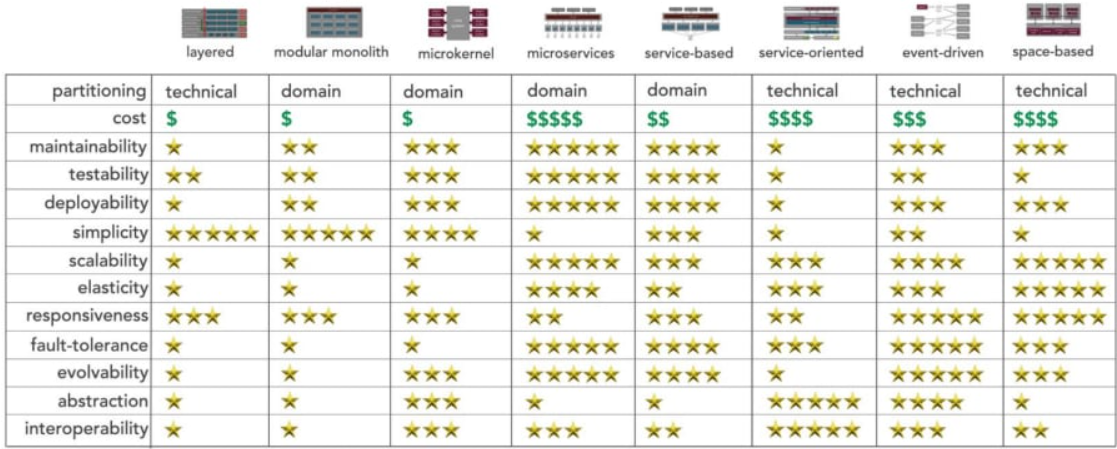
\includegraphics[width=\linewidth]{figures/ch05/architecture/compare-architecture.png}
\caption{So sánh các đặc tính của các kiểu kiến trúc (Nguồn: Mark Richards, Neal Ford, \textit{Fundamentals of Software Architecture}, O'Reilly, 2nd ed., 2020) \cite{Richards2020FSA}.}
\label{fig:compare-architecture}
\end{figure}


\textbf{C. Phân tích loại trừ:}
Từ biểu đồ trên kết hợp với các yêu cầu nghiệp vụ đã xác định, nhóm tiến hành loại trừ các kiến trúc không phù hợp:
\begin{itemize}
    \item \textbf{Loại bỏ Kiến trúc Vi dịch vụ (Microservices):}
    \begin{itemize}
        \item \textit{Ưu điểm từ biểu đồ:} Đạt điểm tuyệt đối về khả năng mở rộng (scalability: 5 sao), triển khai độc lập (deployability: 5 sao), và khả năng chịu lỗi (fault-tolerance: 5 sao).
        \item \textit{Nhược điểm nghiêm trọng:} Chi phí vận hành ở mức cao nhất (\$\$\$\$\$) và độ phức tạp có điểm thấp nhất (simplicity: 1 sao).
        \item \textit{Mâu thuẫn với yêu cầu:} Với nguồn lực hạn chế của đồ án sinh viên, việc vận hành hạ tầng phân tán (service discovery, distributed tracing, container orchestration) là không khả thi. Hơn nữa, các nghiệp vụ mượn/trả sách đòi hỏi cập nhật đồng thời nhiều aggregate (giao dịch, tồn kho, hàng đợi) - nếu tách thành microservices sẽ phải xử lý distributed transactions phức tạp (Saga pattern, 2PC:Two-Phase Commit) với rủi ro eventual consistency.
    \end{itemize}

    \item \textbf{Loại bỏ Kiến trúc Phân lớp (Layered) truyền thống:}
    \begin{itemize}
        \item \textit{Ưu điểm từ biểu đồ:} Đơn giản nhất (simplicity: 5 sao) và chi phí thấp nhất (cost: \$).
        \item \textit{Nhược điểm nghiêm trọng:} Các chỉ số quan trọng cho sự phát triển dài hạn đều ở mức thấp: khả năng bảo trì (maintainability: 1 sao), khả năng kiểm thử (testability: 2 sao), và tính linh hoạt (evolvability: 1 sao).
        \item \textit{Mâu thuẫn với yêu cầu:} Kiến trúc phân lớp theo kỹ thuật (technical layers) dễ dẫn đến tight coupling giữa các logic nghiệp vụ. Đối với hệ thống có yêu cầu tích hợp AI phức tạp (xử lý bất đồng bộ PDF, cập nhật vector embeddings, trigger recommendation engine), kiến trúc này dễ dẫn đến "big ball of mud" với business logic rải rác khắp các layer.
    \end{itemize}

    \item \textbf{Cân nhắc về Kiến trúc Hướng dịch vụ (Service-Based):}
    \begin{itemize}
        \item \textit{Ưu điểm từ biểu đồ:} Sự cân bằng tốt với hầu hết chỉ số đạt 3--4 sao (maintainability: 4 sao, testability: 4 sao, deployability: 4 sao) và chi phí vừa phải (cost: \$\$).
        \item \textit{Hạn chế trong bối cảnh dự án:} Việc tách ngay từ đầu toàn bộ các nghiệp vụ thư viện thành nhiều service riêng biệt (User Service, Catalog Service, Circulation Service, Fine Service) là \textbf{over-engineering} cho giai đoạn MVP. Các service này có phụ thuộc lẫn nhau cao: mượn sách cần kiểm tra tài khoản, tình trạng bản sao, đặt trước và phí phạt. Nếu tách quá sớm, hệ thống sẽ phải đánh đổi bằng nhiều inter-service calls, tăng network latency và độ phức tạp debugging.
        \item \textit{Kết luận:} Service-Based là hướng đi tương lai hợp lý khi hệ thống cần scale, nhưng chưa phù hợp cho giai đoạn đầu.
    \end{itemize}
\end{itemize}

\textbf{D. Quyết định: Kiến trúc Modular Monolith kết hợp Dịch vụ vệ tinh AI}

Dựa trên phân tích trên, nhóm quyết định áp dụng một cách tiếp cận \textbf{thực dụng và có định hướng phát triển}, kết hợp ưu điểm của Modular Monolith với tính linh hoạt của Service-Based Architecture:

\begin{enumerate}
    \item \textbf{Lõi hệ thống: Modular Monolith (Spring Boot)}

    Đây là kiến trúc chủ đạo cho các nghiệp vụ quản lý thư viện (Auth/User, Catalog, Circulation, Fine/Payment, Notification và Engagement).

    \textit{Lý do lựa chọn dựa trên biểu đồ so sánh:}
    \begin{itemize}
        \item \textbf{Cân bằng tối ưu:} Modular Monolith cung cấp maintainability (3 sao) và evolvability (3 sao) tốt hơn hẳn Layered Architecture (1 sao) nhưng vẫn giữ được chi phí thấp (cost: \$) và độ đơn giản cao (simplicity: 5 sao).
        \item \textbf{Testability:} Đạt 3 sao - cao hơn đáng kể so với Layered (2 sao) nhờ tách biệt rõ ràng giữa các domain module.
        \item \textbf{Deployability:} Dù chỉ đạt 3 sao (thấp hơn Microservices), nhưng lại phù hợp với nguồn lực đồ án: chỉ cần deploy một artifact duy nhất, không cần orchestration phức tạp.
    \end{itemize}

    \textit{Lợi ích nghiệp vụ cụ thể:}
    \begin{itemize}
        \item \textbf{Tính nhất quán giao dịch (ACID):} Các use case phức tạp như trả sách (cần atomic update: trạng thái giao dịch + tính phạt + cập nhật tồn kho + trigger hàng đợi) được đảm bảo trong một transaction duy nhất mà không cần distributed transaction protocols.
        \item \textbf{Tính module hóa cao:} Mặc dù là monolith, code được tổ chức theo \textbf{domain boundaries} (không phải technical layers). Mỗi module (Auth/User, Catalog, Circulation, Recommendation...) có domain model, use cases, và repositories riêng, giao tiếp thông qua well-defined interfaces. Điều này tạo "exit strategy" - dễ dàng tách module ra thành service riêng trong tương lai nếu cần.
        \item \textbf{DevOps đơn giản:} Chỉ cần một deployment pipeline, một database connection pool, không cần service mesh hay API gateway phức tạp.
    \end{itemize}

    \item \textbf{Dịch vụ vệ tinh: AI Service (Python/FastAPI)}

    Mô-đun AI/Recommendation System được tách ra thành một dịch vụ độc lập, giao tiếp với Monolith chủ yếu qua REST API. Các tác vụ xử lý PDF được backend kích hoạt bất đồng bộ sau khi lưu URL tài liệu; AI service cũng có khả năng chạy worker nền cho các job xử lý dài nếu cần.

    \textit{Lý do tách riêng:}
    \begin{itemize}
        \item \textbf{Công nghệ khác biệt:} Hệ sinh thái Python (HuggingFace/SentenceTransformer, PyMuPDF, implicit ALS, FastAPI) phù hợp hơn cho ML/NLP so với việc nhúng các thư viện này trực tiếp vào Spring Boot.
        \item \textbf{Scaling requirements khác biệt:} AI workload (PyMuPDF, vector similarity search, model inference) tiêu tốn CPU/GPU nhiều hơn CRUD nghiệp vụ. Tách riêng cho phép scale độc lập (horizontal scaling với GPU instances) mà không tốn tài nguyên cho monolith.
        \item \textbf{Bất đồng bộ tự nhiên:} Xử lý PDF, sinh embedding và gọi Gemini không cần chặn luồng thủ thư upload tài liệu. Backend lưu trạng thái ETL, gọi AI service bằng tác vụ nền và có fallback khi AI lỗi.
        \item \textbf{Tính module hóa:} AI Service dùng schema dữ liệu phục vụ AI như \texttt{ai\_engine.publication\_vectors}, \texttt{publication\_etl\_runs} và bảng \texttt{ai\_recommendations}, nhưng giao tiếp với backend vẫn thông qua API contract rõ ràng. Nhờ đó nhóm có thể thay đổi model embedding hoặc chiến lược recommendation mà không làm xáo trộn nghiệp vụ thư viện.
    \end{itemize}

    \textit{Migration path:} Đây là bước đệm hướng tới Service-Based Architecture. Trong tương lai, nếu cần scale, có thể tách dần các module khác (User Service, Notification Service) ra khỏi monolith theo pattern tương tự.
\end{enumerate}


\textbf{E. Đánh giá kiến trúc lai theo các chỉ số:}
Kiến trúc Modular Monolith + AI Satellite này đạt được sự cân bằng tốt nhất cho bối cảnh dự án:
\begin{table}[H]
\centering
\caption{Đánh giá kiến trúc lai so với các chỉ số}
\begin{tabular}{|l|c|l|}
\hline
\textbf{Tiêu chí} & \textbf{Điểm} & \textbf{Nhận xét} \\ \hline
Cost & \$\$ & Giữa Modular Monolith (\$) và Service-Based (\$\$), phù hợp ngân sách \\ \hline
Simplicity & 3-4 sao & Đơn giản hơn Microservices nhưng cần quản lý 2 components \\ \hline
Maintainability & 3-4 sao & Module hóa domain tốt, dễ sửa lỗi và refactor \\ \hline
Testability & 3 sao & Domain logic tách biệt, dễ unit test \\ \hline
Deployability & 2-3 sao & Deploy 2 artifacts (Monolith + AI), CI/CD đơn giản \\ \hline
Scalability & 3 sao & AI service scale độc lập, monolith scale theo nhu cầu \\ \hline
Evolvability & 4 sao & Có thể tách dần modules ra thành services khi cần \\ \hline
\end{tabular}
\end{table}

\textbf{Kết luận:} Kiến trúc Modular Monolith + AI Satellite Service đạt được ba mục tiêu then chốt: (1) Đảm bảo tính nhất quán giao dịch cho nghiệp vụ core, (2) Tối ưu hóa AI workload với công nghệ và scaling phù hợp, (3) Giữ độ phức tạp và chi phí ở mức chấp nhận được cho đồ án, đồng thời tạo nền tảng để mở rộng thành Service-Based Architecture hoặc Microservice Architecture trong tương lai.


\subsection{Thiết kế cơ sở dữ liệu}
\label{subsec:database-design}

Thiết kế cơ sở dữ liệu là quá trình chuyển đổi từ mô hình phân tích yêu cầu và các thực thể đã được đặc tả ở các phần trước thành một cấu trúc lưu trữ logic và vật lý. Mục tiêu là xây dựng một nền tảng dữ liệu nhất quán, toàn vẹn, hiệu quả và có khả năng mở rộng để hỗ trợ toàn bộ nghiệp vụ của hệ thống, từ các giao dịch mượn trả cơ bản đến các tính năng AI phức tạp.

\subsubsection{Lựa chọn Hệ Quản trị Cơ sở dữ liệu (HQTCSDL)}
Dựa trên bản chất quan hệ chặt chẽ của dữ liệu (người dùng, sách, lượt mượn), hệ thống lựa chọn \textbf{PostgreSQL} làm HQTCSDL chính.
\begin{itemize}
 \item \textbf{Tính tin cậy và toàn vẹn dữ liệu:} PostgreSQL nổi tiếng với sự tuân thủ nghiêm ngặt các tiêu chuẩn ACID (Atomicity, Consistency, Isolation, Durability), đảm bảo các giao dịch nghiệp vụ quan trọng như mượn, trả, và tính phí phạt luôn được thực hiện một cách an toàn.
 \item \textbf{Hỗ trợ các kiểu dữ liệu nâng cao:} PostgreSQL hỗ trợ các kiểu dữ liệu phức tạp như JSONB, rất hữu ích để lưu trữ các metadata linh hoạt. Đặc biệt, thông qua các extension như \texttt{pgvector}, nó có khả năng lưu trữ và truy vấn các vector embedding hiệu quả, phục vụ trực tiếp cho tính năng tìm kiếm ngữ nghĩa.
 \item \textbf{Khả năng mở rộng:} Đây là một hệ quản trị CSDL mã nguồn mở mạnh mẽ, đã được chứng minh về hiệu năng trong các hệ thống quy mô lớn.
\end{itemize}

\subsubsection{Mô hình Quan hệ Thực thể (ERD)}
Bên dưới là sơ đồ ERD tổng quan của toàn bộ hệ thống. Mô hình dữ liệu được
thiết kế xoay quanh thực thể trung tâm là \textbf{Publication} và
\textbf{User}. \textbf{Publication} biểu diễn đầu sách hoặc tài liệu thư viện,
liên kết với tác giả, nhà xuất bản, danh mục, thẻ chủ đề, bản sao vật lý
(\textbf{Item}) và dữ liệu vector phục vụ tìm kiếm ngữ nghĩa. \textbf{User}
liên kết với vai trò, lịch sử tìm kiếm, wishlist, đánh giá, tương tác, thông
báo và các nghiệp vụ mượn/đặt trước.

Các quan hệ nghiệp vụ chính được thể hiện qua \textbf{borrowing\_transactions},
\textbf{reservations} và \textbf{fines}. Một người dùng có thể tạo nhiều phiếu
mượn hoặc đặt trước; mỗi phiếu mượn gắn với một bản sao sách cụ thể và có thể
phát sinh phí phạt nếu quá hạn, mất sách hoặc hư hỏng. Nhóm bảng AI như
\textbf{PublicationVector}, \textbf{Ai\_Recommendation} và
\textbf{user\_interactions} được tách ra nhưng vẫn liên kết với dữ liệu lõi để
hỗ trợ gợi ý cá nhân hóa, tìm kiếm ngữ nghĩa và phân tích hành vi đọc.

\begin{figure}[htbp]
 \centering
\includegraphics[width=1\linewidth]{figures/ch05/database/erd.png}
 \caption{Sơ đồ Quan hệ Thực thể (ERD) tổng thể của hệ thống}
 \label{fig:erd}
\end{figure}
\FloatBarrier

\subsection{Thiết kế chi tiết bên trong}
\subsubsection{Mô hình kiến trúc chi tiết}
Sau khi quyết định sử dụng kiến trúc Modular Monolith kết hợp AI Satellite Service, phần này trình bày chi tiết cấu trúc nội bộ của từng thành phần và các nguyên tắc thiết kế được áp dụng.

\textbf{A. Tổng quan kiến trúc hệ thống:}
\begin{figure}[htbp]
 \centering
 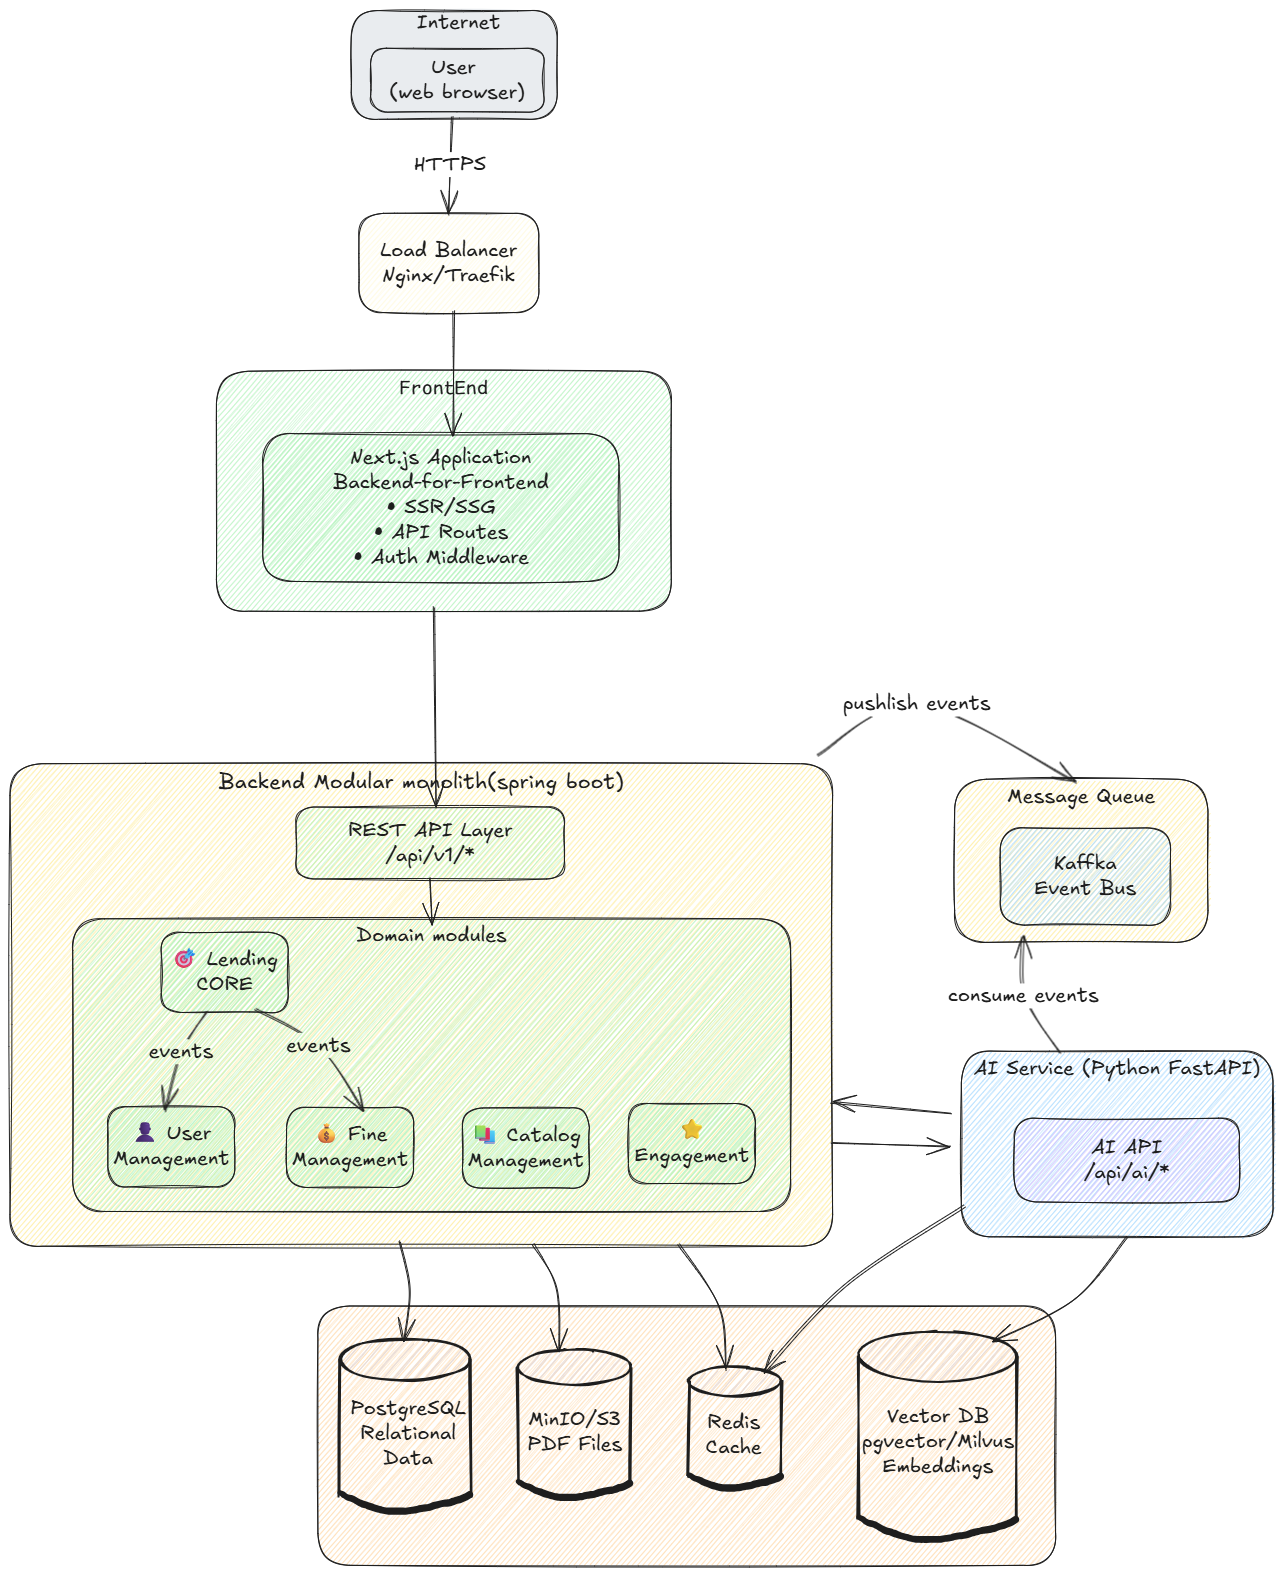
\includegraphics[width=1\linewidth]{figures/ch05/architecture/system_architecture_overview.png}
 \caption{Sơ đồ kiến trúc tổng thể hệ thống}
 \label{fig:system_architecture_overview}
\end{figure}
Hệ thống bao gồm ba thành phần chính:
\begin{enumerate}
    \item \textbf{Frontend (React/Vite SPA):} Giao diện người dùng chạy phía trình duyệt, tổ chức route cho public, reader, librarian và admin, gọi REST API trực tiếp đến backend.
    \item \textbf{Backend Monolith (Spring Boot):} Lõi nghiệp vụ áp dụng Domain-Driven Design và Clean Architecture.
    \item \textbf{AI Service (Python FastAPI):} Dịch vụ độc lập xử lý các tác vụ Machine Learning và Vector Search.
\end{enumerate}


\textbf{B. Kiến trúc Backend Monolith (Spring Boot)}
\textbf{Tổ chức theo Bounded Contexts (DDD):}

Thay vì tổ chức code theo các lớp kỹ thuật ngang (technical layers), hệ thống được chia thành các module theo ranh giới nghiệp vụ (domain boundaries), mỗi module tương ứng với một Bounded Context trong Domain-Driven Design:

\begin{figure}[htbp]
 \centering
 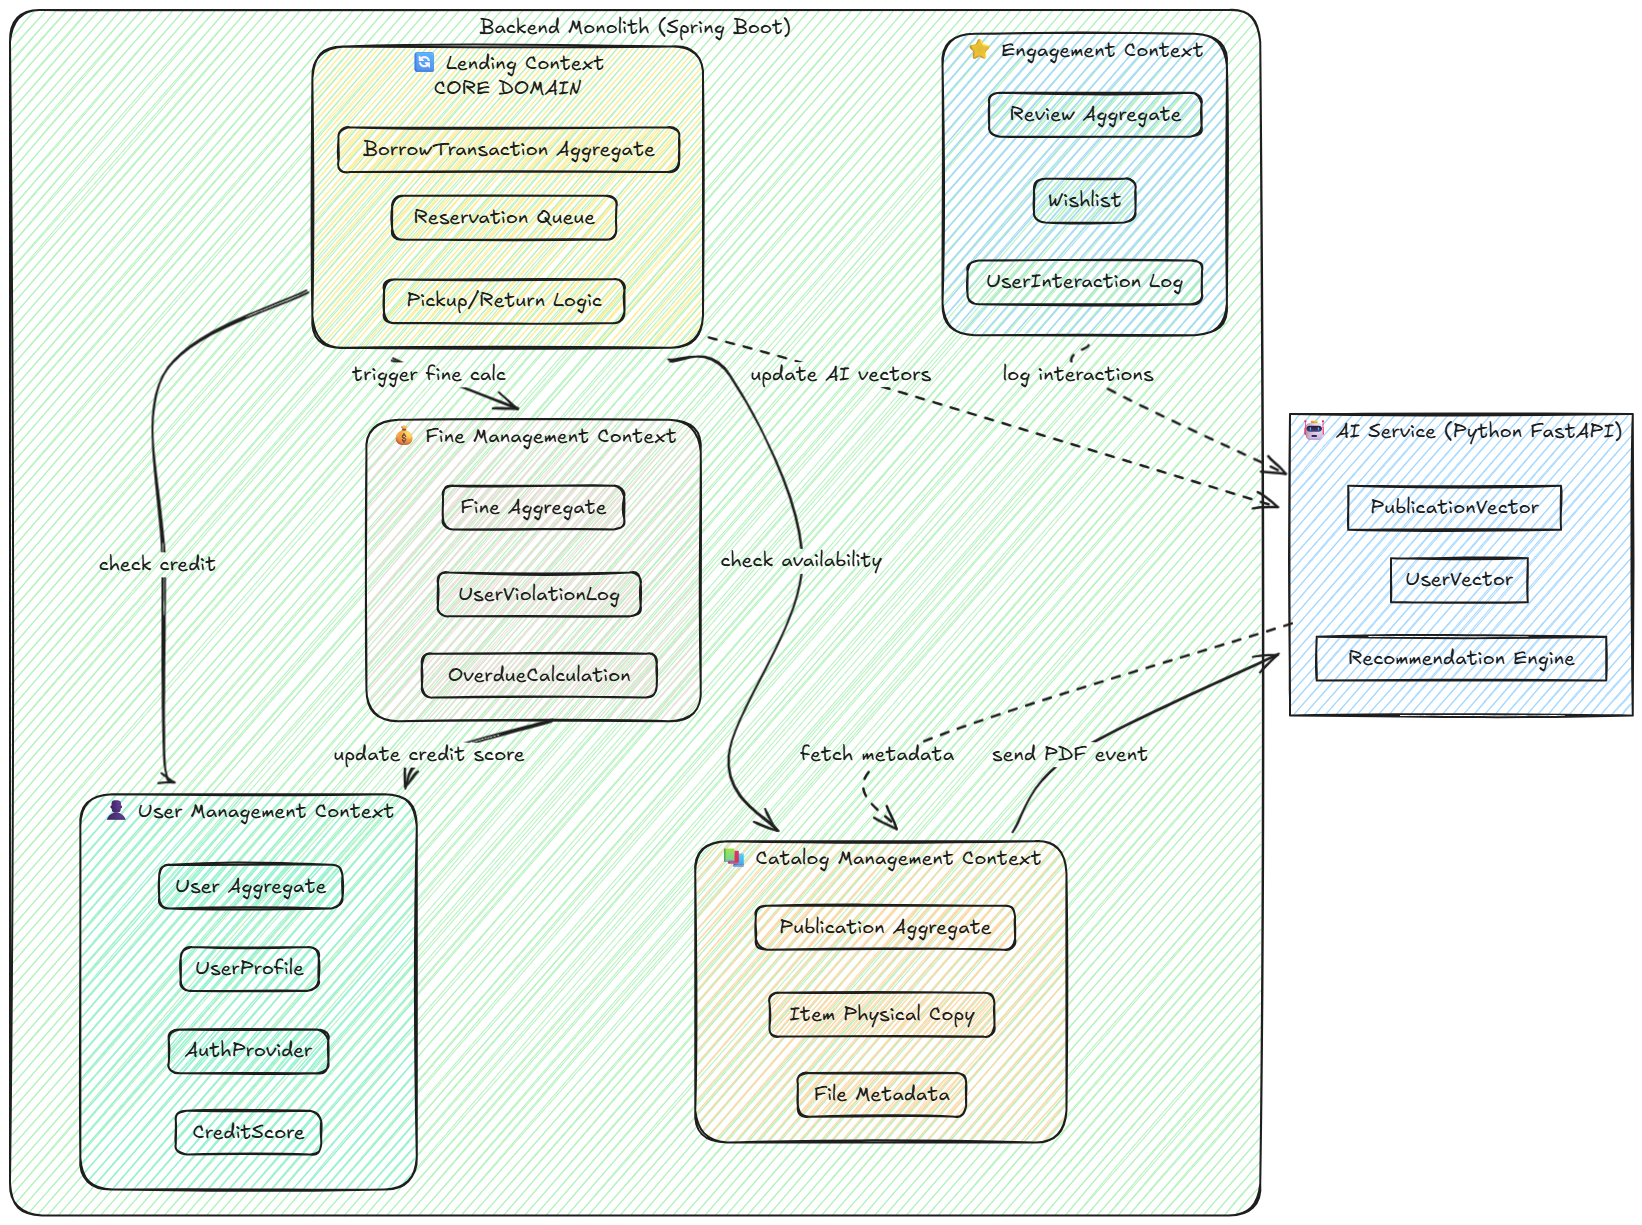
\includegraphics[width=1\linewidth]{figures/ch05/architecture/bounded_contexts.png}
 \caption{Các Bounded Contexts trong hệ thống}
 \label{fig:bounded_contexts}
\end{figure}

\begin{itemize}
    \item \textbf{Auth/User Management Context:} Quản lý đăng ký, đăng nhập, xác thực email, Google OAuth, hồ sơ người dùng, vai trò và phân quyền.
    \item \textbf{Catalog Management Context:} Quản lý thông tin xuất bản phẩm (Publication), các bản sao vật lý (Item), metadata sách, và file storage.
    \item \textbf{Circulation Context:} \textit{(Core Domain)} - Quản lý vòng đời mượn/trả sách (BorrowingTransaction), yêu cầu mượn, xác nhận nhận sách, hàng đợi đặt trước (Reservation), trả sách và báo cáo sách hư/mất.
    \item \textbf{Fine/Payment Context:} Quản lý phí quá hạn, phí sự cố, thanh toán tiền mặt, thanh toán PayOS và đồng bộ trạng thái webhook.
    \item \textbf{Engagement/Recommendation Context:} Quản lý đánh giá sách, phản hồi review, danh sách yêu thích, lịch sử tìm kiếm, log tương tác người dùng, semantic search và recommendation.
    \item \textbf{Notification Context:} Lưu thông báo, đếm thông báo chưa đọc và đẩy realtime qua WebSocket/STOMP.
\end{itemize}

Mỗi Bounded Context được thiết kế như một "mini-service" bên trong monolith, có thể tách ra thành service độc lập trong tương lai mà không cần refactor lớn.

\textbf{Clean Architecture bên trong mỗi Module:}

Bên trong mỗi Bounded Context, code được tổ chức theo 4 layers của Clean Architecture để đảm bảo tách biệt trách nhiệm và independence từ framework/database:
\begin{figure}[htbp]
 \centering
 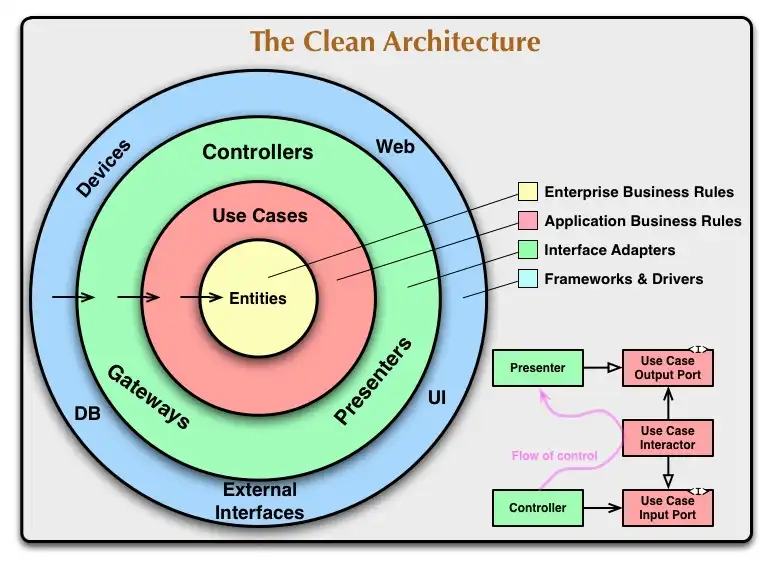
\includegraphics[width=1\linewidth]{figures/ch05/architecture/clean-architecture.png}
 \caption{Clean architecture (R. C. Martin, \textit{Clean Architecture: A Craftsman’s Guide to Software Structure and Design},  Pearson Education, 2018 \cite{martin2018clean})}
 \label{fig:clean_architecture_layers}
\end{figure}
\begin{figure}[htbp]
 \centering
 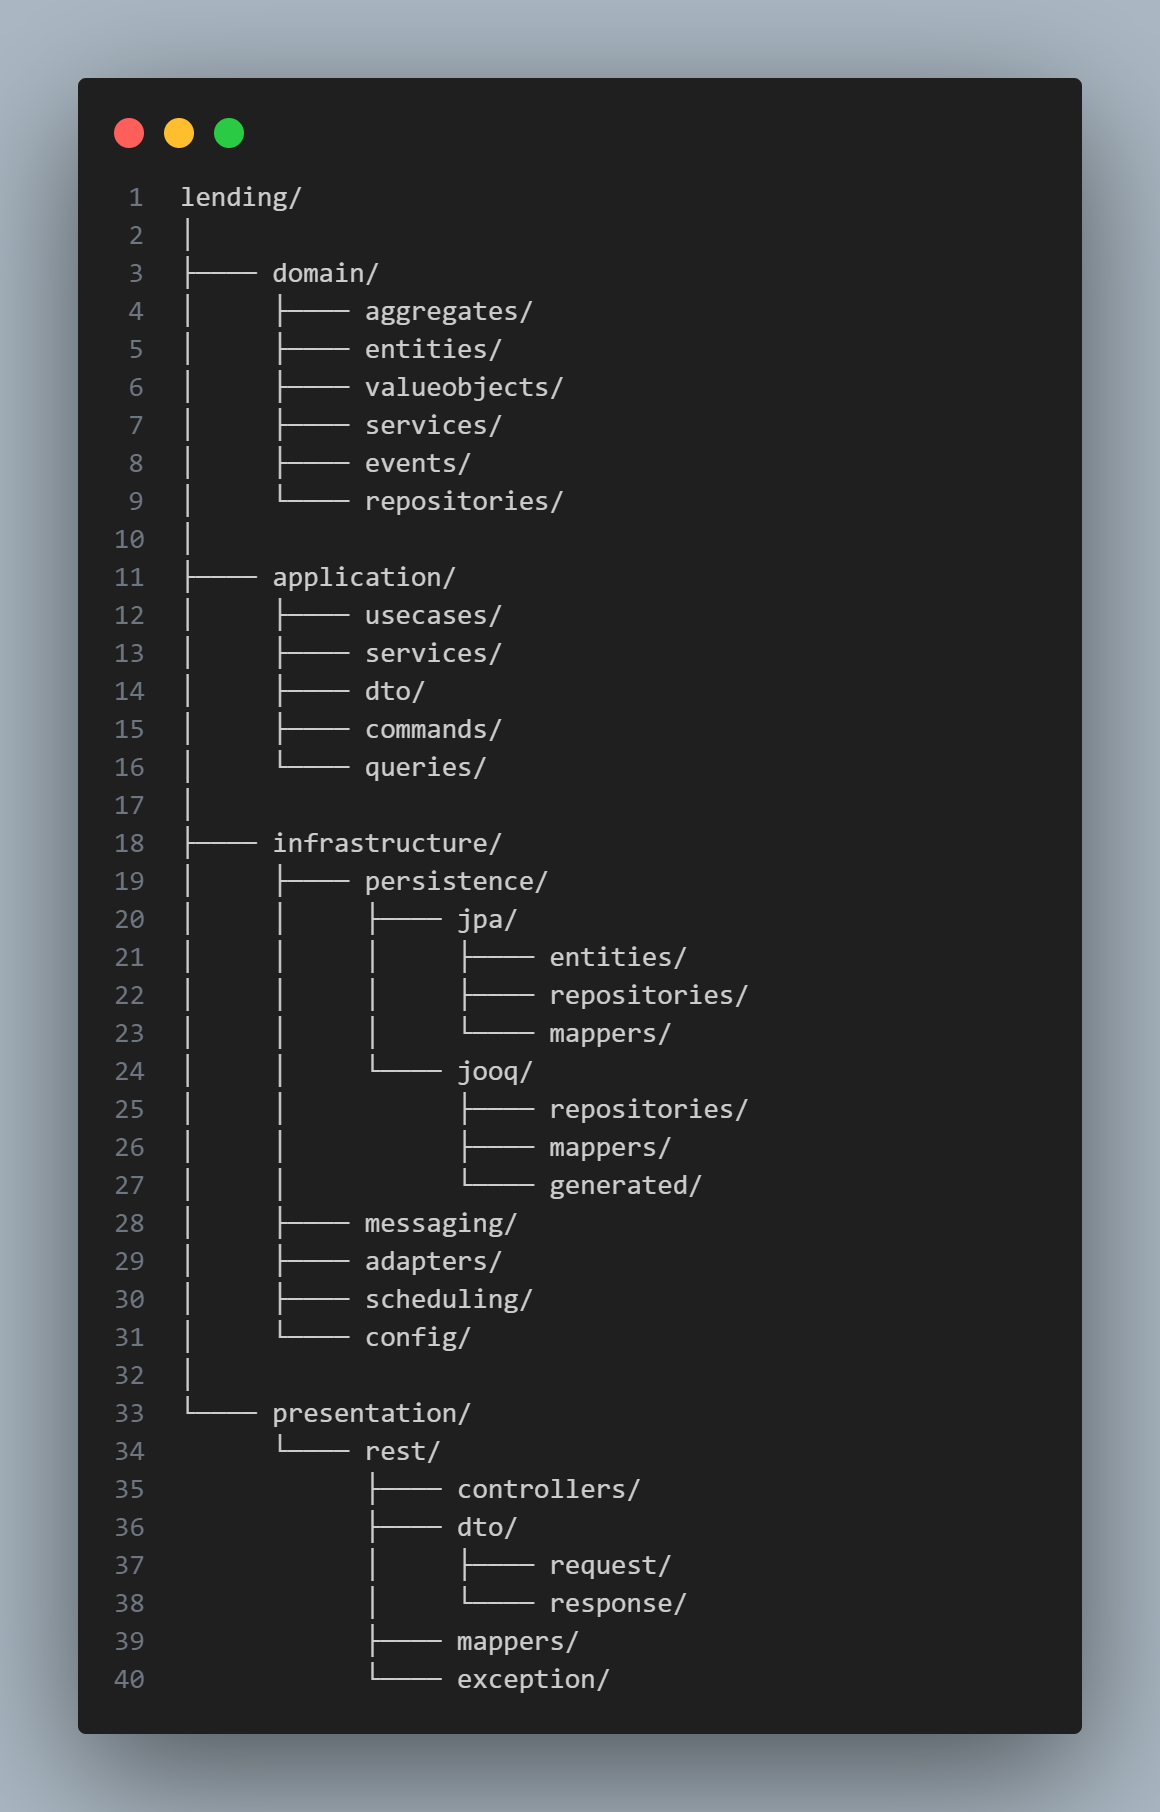
\includegraphics[width=0.8\linewidth]{figures/ch05/architecture/folder_structure_backend.png}
 \caption{Cấu trúc Clean Architecture kết hợp Domain-Driven Design trong một Module}
 \label{fig:clean_architecture_in_module}
\end{figure}

\textbf{1. Domain Layer (Lõi nghiệp vụ - Innermost):}
\begin{itemize}
    \item \textbf{Entities và Aggregates:} Chứa các đối tượng nghiệp vụ cốt lõi với business invariants. Ví dụ:
    \begin{itemize}
        \item \texttt{BorrowingTransaction} Aggregate: Đảm bảo vòng đời giao dịch từ yêu cầu mượn, xác nhận nhận sách, đang mượn, trả sách đến báo cáo sự cố.
        \item \texttt{Publication} Aggregate: Đảm bảo metadata ấn phẩm nhất quán, liên kết đúng tác giả, nhà xuất bản, danh mục, tag, ảnh bìa và tài liệu PDF.
        \item \texttt{Item} Aggregate: Đảm bảo mỗi bản sao có barcode riêng, trạng thái riêng và chỉ được mượn khi đang khả dụng.
    \end{itemize}

    \item \textbf{Value Objects:} Các đối tượng bất biến đại diện cho khái niệm nghiệp vụ không có identity riêng, ví dụ \texttt{Barcode}, \texttt{PublicationId}, \texttt{ItemId} hoặc trạng thái bản sao.

    \item \textbf{Domain Services:} Logic nghiệp vụ thuần không thuộc về một Entity/Aggregate cụ thể. Ở mức thiết kế, nhóm dự kiến đặt tại đây các quy tắc có thể dùng lại như:
    \begin{itemize}
        \item Tính số ngày quá hạn và xác định loại phí phát sinh theo chính sách lưu thông.
        \item Chọn bản sao phù hợp cho yêu cầu đặt trước dựa trên trạng thái bản sao, chi nhánh và thứ tự hàng đợi.
    \end{itemize}

    \item \textbf{Domain Events:} Biểu diễn các sự kiện nghiệp vụ quan trọng để application/infrastructure có thể phản ứng mà không làm domain phụ thuộc vào công nghệ cụ thể:
    \begin{itemize}
        \item Sự kiện mượn/trả, phát sinh phí phạt, thay đổi trạng thái đặt trước.
        \item Sự kiện yêu cầu gửi thông báo/email sau khi transaction nghiệp vụ hoàn tất.
        \item Sự kiện thay đổi trạng thái xử lý tài liệu sau khi pipeline AI hoàn tất hoặc thất bại.
    \end{itemize}

    \item \textbf{Repository Interfaces:} Domain định nghĩa các interface (contract) mà Infrastructure sẽ implement. Domain không quan tâm dùng JPA, JDBC hay MongoDB.

    \item \textbf{Ràng buộc nghiêm ngặt:} Domain Layer KHÔNG ĐƯỢC phụ thuộc vào bất kỳ layer nào khác, không import Spring annotations, không biết HTTP hay Database. Đây là "business logic in pure Java".
\end{itemize}

\textbf{2. Application Layer (Use Cases - Orchestrator):}
\begin{itemize}
    \item \textbf{Use Case Services:} Mỗi use case là một entry point cho một chức năng nghiệp vụ hoàn chỉnh. Ví dụ:
    \begin{itemize}
        \item \texttt{BorrowRequestUseCase}: Điều phối luồng gửi yêu cầu mượn từ bạn đọc.
        \item \texttt{BorrowDirectUseCase}: Điều phối luồng thủ thư cho mượn trực tiếp tại quầy.
        \item \texttt{ConfirmPickupUseCase}: Xác nhận bạn đọc đã nhận sách sau khi có yêu cầu mượn hoặc đặt trước.
        \item \texttt{ReturnBookUseCase}: Điều phối luồng trả sách, cập nhật bản sao và tính phí quá hạn nếu có.
        \item \texttt{ReportIssueUseCase}: Ghi nhận sách hư/mất và tạo phí sự cố.
    \end{itemize}

    \item \textbf{Trách nhiệm chính:}
    \begin{itemize}
        \item Orchestrate workflow: Gọi repositories để load aggregates, gọi domain services, và save kết quả.
        \item Quản lý transaction boundaries (sử dụng \texttt{@Transactional} annotation của Spring).
        \item Kích hoạt các side effect cần thiết như notification, email hoặc cập nhật trạng thái AI thông qua adapter tương ứng.
        \item Transform exceptions: Chuyển domain exceptions thành application-level error codes.
    \end{itemize}

    \item \textbf{Application Services:} Các facade cho phép module khác gọi vào (public API giữa các modules).

    \item \textbf{DTOs (Data Transfer Objects):} Chuyển đổi giữa domain objects và external representations (JSON, DTO cho API).

    \item \textbf{Lưu ý:} Application Layer được phép phụ thuộc vào Domain Layer và định nghĩa interfaces cho Infrastructure (Dependency Inversion Principle).
\end{itemize}


\textbf{3. Infrastructure Layer (Technical Implementation - Outermost):}
\begin{itemize}
    \item \textbf{Repository Implementations:} Hiện thực các repository interfaces từ Domain bằng JPA/Hibernate, JDBC, hoặc bất kỳ persistence technology nào. Ví dụ:
    \begin{itemize}
        \item \texttt{BorrowingTransactionJpaRepository}: Truy vấn và cập nhật giao dịch mượn--trả.
        \item Mapping giữa domain/use case và JPA Entity như \texttt{BorrowingTransactionEntity}, \texttt{FineEntity}, \texttt{PublicationEntity}.
    \end{itemize}

    \item \textbf{External Service Adapters:} Tích hợp với các dịch vụ bên ngoài:
    \begin{itemize}
        \item Email/SMS Service (gửi notification)
        \item File Storage (S3-compatible storage để lưu ảnh bìa và PDF)
        \item Payment Gateway (PayOS cho thanh toán phạt trực tuyến)
        \item OAuth Provider (Google Authentication)
    \end{itemize}

    \item \textbf{Event Infrastructure:} Hiện thực event publishing/subscribing:
    \begin{itemize}
        \item Kafka producer/consumer cho notification, email và các tác vụ cần tách khỏi request chính.
        \item REST client đến AI Service cho semantic search, recommendation và xử lý PDF.
    \end{itemize}

    \item \textbf{Technical Services:}
    \begin{itemize}
        \item Scheduler (Spring \texttt{@Scheduled}) cho background jobs (check overdue daily).
        \item WebSocket/STOMP cho thông báo realtime.
        \item Security (JWT token generation/validation, password hashing).
    \end{itemize}

    \item \textbf{Configuration:} Database connection pools, Kafka/WebSocket configuration, S3, PayOS, AI gateway, security settings.
\end{itemize}


\textbf{4. Presentation Layer (Interface Adapters):}
\begin{itemize}
    \item \textbf{REST Controllers:} Expose các use cases qua HTTP/REST API. Mỗi Bounded Context có controller riêng:
    \begin{itemize}
        \item \texttt{UserController} (\texttt{/api/v1/users/*})
        \item \texttt{PublicationController} (\texttt{/api/v1/publications/*})
        \item \texttt{BorrowingTransactionController} (\texttt{/api/v1/transactions/*})
        \item \texttt{ReservationController} (\texttt{/api/v1/reservations/*})
        \item \texttt{FineController} (\texttt{/api/v1/fines/*})
        \item \texttt{RecommendationController} (\texttt{/api/v1/recommendations/*})
        \item \texttt{AiSearchController} (\texttt{/api/v1/ai/semantic-search})
    \end{itemize}

    \item \textbf{Trách nhiệm:}
    \begin{itemize}
        \item Nhận HTTP requests, validate syntax (JSON format, required fields, regex).
        \item Chuyển đổi Request DTOs → Commands/Queries cho Application Layer.
        \item Authentication \& Authorization: Extract user info từ JWT, check permissions.
        \item Chuyển đổi kết quả từ Application Layer → HTTP Response (JSON).
        \item Error handling: Chuyển exceptions thành HTTP status codes (400, 401, 403, 404, 500).
    \end{itemize}

    \item \textbf{Nguyên tắc:} Controllers phải "thin" - chỉ làm việc chuyển đổi và delegation, KHÔNG chứa business logic.
\end{itemize}

\textbf{Dependency Rule (Nguyên tắc phụ thuộc):}
Clean Architecture tuân thủ nguyên tắc: \textbf{Dependencies chỉ được point inward} (từ ngoài vào trong):

\begin{center}
\texttt{Presentation → Application → Domain ← Infrastructure}
\end{center}

\begin{itemize}
    \item Domain Layer: Không phụ thuộc vào ai (pure business logic).
    \item Application Layer: Chỉ phụ thuộc Domain, định nghĩa interfaces cho Infrastructure.
    \item Infrastructure \& Presentation: Phụ thuộc cả Domain và Application, implement interfaces.
\end{itemize}

Điều này đảm bảo business logic (Domain) không bị "ô nhiễm" bởi framework, database hay HTTP concerns.


%-----------------------------AI-----------------------------------


\textbf{C. Kiến trúc AI Service (Python FastAPI)}
Hệ thống AI Service được thiết kế như một \textit{Dịch vụ Vệ tinh Độc lập} (AI Satellite Service), tách biệt khỏi khối Monolith (Spring Boot). Quyết định này nhằm tận dụng sức mạnh của hệ sinh thái Python trong các tác vụ Học máy (Machine Learning) và Xử lý ngôn ngữ tự nhiên (NLP), đồng thời đảm bảo khả năng mở rộng độc lập cho các tác vụ tính toán nặng.
\textbf{C.1. Chiến lược thiết kế và Lựa chọn công nghệ}
Khác với Backend chính tập trung vào tính toàn vẹn dữ liệu giao dịch, AI Service tập trung vào hiệu năng tính toán ma trận và xử lý bất đồng bộ.
\begin{itemize}
\item \textbf{Web Framework - FastAPI:} Được lựa chọn thay vì Flask/Django vì nhẹ, dễ định nghĩa API contract, hỗ trợ Pydantic để kiểm soát dữ liệu đầu vào và phù hợp với các endpoint inference như semantic search, recommendation và publication processing.
\item \textbf{Kiến trúc Phi trạng thái (Stateless):} AI Service không lưu trữ session người dùng. Mọi trạng thái cần thiết được truyền qua payload của request hoặc truy xuất từ PostgreSQL/model artifact, giúp dễ dàng mở rộng theo chiều ngang (Horizontal Scaling) bằng cách tăng số lượng container.
\end{itemize}
\textbf{C.2. Cấu trúc Phân tầng (Layered Architecture)} \\
Kiến trúc nội bộ của AI Service được tinh gọn thành 3 tầng chính để tối ưu hóa đường đi của dữ liệu: \\
\textbf{a. API Layer (Giao tiếp \& Định tuyến):}
\begin{itemize}
\item \textit{Semantic Search Router:} \texttt{POST /api/v1/semantic-search}
\begin{itemize}
\item Xử lý truy vấn tìm kiếm bằng ngôn ngữ tự nhiên.
\item Pipeline: Tiền xử lý text $\rightarrow$ Encoding $\rightarrow$ Vector Search.
\end{itemize}
\item \textit{Recommendation Router:} \texttt{POST /api/v1/recommendations}
\begin{itemize}
\item Trả về danh sách gợi ý cá nhân hóa dựa trên ngữ cảnh (Trang chủ, Chi tiết sách).
\item Có thể mở rộng thêm endpoint làm mới gợi ý theo người dùng khi cần cập nhật mô hình hoặc dữ liệu tương tác.
\end{itemize}
\item \textit{Similar Publications Router:} \texttt{GET /api/v1/publications/\{publicationId\}/similar}
\begin{itemize}
\item Trả về các ấn phẩm tương tự với một sách cụ thể, phục vụ khối gợi ý ở trang chi tiết sách.
\end{itemize}
\item \textit{Data Ingestion Router:} \texttt{POST /api/v1/publications/process}
\begin{itemize}
\item Endpoint nhận yêu cầu xử lý tài liệu mới, trích xuất text PDF, sinh metadata AI và lưu embedding.
\end{itemize}
\end{itemize}
\textbf{b. Service Layer (Logic nghiệp vụ ML):}
Đây là trái tim của hệ thống, chứa các pipeline xử lý dữ liệu phức tạp:
\begin{itemize}
\item \textbf{Embedding Service:} Sử dụng mô hình \texttt{bkai-foundation-models/vietnamese-bi-encoder} hoặc mô hình tương đương để chuyển đổi văn bản tiếng Việt thành vector 768 chiều. Mô hình được load một lần khi service/worker khởi động để giảm độ trễ suy luận.
\item \textbf{PDF Processing Pipeline:}
\begin{itemize}
\item \textit{Extraction:} Sử dụng \textbf{PyMuPDF} để trích xuất văn bản tốc độ cao (nhanh hơn 10x so với pypdf).
\item \textit{Chunking:} Áp dụng chiến lược Cửa sổ trượt theo ký tự với kích thước chunk 1500 và overlap 150 để bảo toàn ngữ cảnh giữa các đoạn cắt.
\item \textit{Metadata Reduce:} Chọn các chunk đại diện, gửi một prompt chính đến Gemini để tạo summary, audience và tag; nếu Gemini lỗi, hệ thống dùng fallback deterministic.
\end{itemize}
\item \textbf{Recommendation Engine:} Sử dụng thư viện \textbf{implicit} để huấn luyện mô hình ALS cho dữ liệu phản hồi ẩn, kết hợp thêm content-based recommendation và trending fallback cho người dùng mới hoặc dữ liệu ít.
\end{itemize}
\textbf{c. Data \& Storage Layer:}
\begin{itemize}
\item \textbf{Vector Database (PostgreSQL + pgvector):} Lưu trữ embeddings của các chunk nội dung PDF. Sử dụng chỉ mục \textbf{HNSW} (Hierarchical Navigable Small World) để tối ưu hóa tốc độ tìm kiếm láng giềng gần nhất (ANN) thay vì quét toàn bộ bảng.
\item \textbf{Model Store:} Các mô hình nặng (SBERT) được tải sẵn vào RAM khi khởi động (Pre-loaded) để giảm độ trễ (Latency).
\item \textbf{Recommendation Store:} Mô hình ALS sau khi huấn luyện được lưu dưới dạng artifact \texttt{.pkl}; kết quả gợi ý gần nhất có thể được lưu lại trong PostgreSQL để backend có dữ liệu fallback khi AI service tạm thời không phản hồi.
\end{itemize}


\begin{figure}[htbp]
\centering
\resizebox{\textwidth}{!}{%
    \begin{tikzpicture}[
      node distance=2.5cm and 2cm,
      auto,
      % Styles
      user/.style={
        rectangle, draw, rounded corners,
        minimum width=2.5cm, minimum height=1.2cm,
        fill=blue!5, align=center, font=\normalsize
      },
      service/.style={
        rectangle, draw, rounded corners,
        minimum width=3.5cm, minimum height=1.5cm,
        fill=gray!10, align=center, font=\normalsize
      },
      db/.style={
        cylinder, shape border rotate=90,
        draw, minimum height=1.5cm,
        minimum width=2cm, align=center,
        fill=orange!10, font=\small, aspect=0.25
      },
      queue/.style={
        rectangle, draw, dashed,
        minimum width=3cm, minimum height=1.2cm,
        fill=red!5, align=center, font=\normalsize
      },
      sync_arrow/.style={
        ->, thick, draw=blue!70, >=stealth
      },
      async_arrow/.style={
        ->, thick, dashed, draw=red!70, >=stealth
      },
      label_text/.style={
        font=\small, align=center, auto=false, fill=white, inner sep=1pt
      }
    ]

    % --- 1. NODES (KHỐI) ---

    % Main flow
    \node[user] (user) {User\\(Browser)};
    \node[service, right=of user] (frontend) {Frontend\\(React/Vite)};
    \node[service, right=of frontend] (backend) {Core Backend\\(Spring Boot)};

    % AI service
    \node[service, below=5cm of backend, fill=green!5, draw=green!60!black] (ai_api) {AI Service API\\(FastAPI)};
    \node[service, below=0.8cm of ai_api, fill=green!5, draw=green!60!black] (ai_worker) {AI Pipeline\\(PDF/Embed)};

    % Group AI
    \node[fit=(ai_api)(ai_worker), draw=green!60!black, dashed, inner sep=0.5cm, label={[green!60!black]above left:\textbf{AI Service}}] (ai_group) {};

    % Async trigger: backend gọi AI sau khi lưu document URL
    \node[queue, right=of backend, xshift=0.5cm, yshift=-2.5cm] (rabbitmq) {Queue/Callback\\(RabbitMQ/Celery)};

    % Storage layer
    \node[db, right=of ai_api, xshift=4.5cm] (pgvector) {Vector DB\\(pgvector)};

    % Metadata and file storage
    \node[db, above=2.5cm of pgvector] (redis) {PostgreSQL\\Metadata};
    \node[db, below=2.5cm of pgvector] (minio) {File Storage\\(S3-compatible)};

    % --- 2. EDGES (KẾT NỐI) ---

    % Synchronous flow
    \draw[sync_arrow] (user) -- node[below] {HTTP} (frontend);
    \draw[sync_arrow] (frontend) -- (backend);

    % Backend -> AI API
    \draw[sync_arrow] (backend) to[bend right=40] node[left, label_text, pos=0.5, xshift=-0.3cm] {1. Search/Rec Req} (ai_api);

    % AI API -> VectorDB
    \draw[sync_arrow] (ai_api) -- node[above, label_text] {2. Query} (pgvector);

    % AI API -> Metadata
    \draw[sync_arrow] (ai_api) |- node[near end, left, label_text, yshift=-0.5cm] {Metadata} (redis);

    % Asynchronous flow

    % A. Backend -> Async trigger
    \draw[async_arrow] (backend) to[bend left=20] node[right, label_text, pos=0.6, xshift=0.2cm] {A. Process PDF} (rabbitmq);

    % B. Trigger -> Worker
    % Đi vòng cung lớn để tránh đè lên chữ khác
    \draw[async_arrow] (rabbitmq.east) to[bend left=50] node[right, label_text, pos=0.5] {B. Execute} (ai_worker.east);

    % C. Pipeline -> File Storage
    \draw[async_arrow] (ai_worker) to[bend right=20] node[below, label_text] {C. Fetch PDF} (minio);

    % D. Worker -> VectorDB
    \draw[async_arrow] (ai_worker) to[bend right=25] node[right, label_text, pos=0.4] {D. Save Vectors} (pgvector);

    % Legend
    \node[draw, fill=white, font=\small, inner sep=6pt,
          below=1cm of minio, xshift=-2cm, anchor=north] {
        \begin{tabular}{@{}l@{\hspace{6pt}}l@{}}
        \tikz[baseline=-0.5ex]{\draw[sync_arrow] (0,0) -- (0.8,0);} & Sync (REST) \\[4pt]
        \tikz[baseline=-0.5ex]{\draw[async_arrow] (0,0) -- (0.8,0);} & Async (Background)
        \end{tabular}
    };

    \end{tikzpicture}
}
\caption{Sơ đồ luồng dữ liệu và Kiến trúc chi tiết AI Service}
\label{fig:ai_service_architecture_diagram}
\end{figure}



\textbf{Sơ đồ chi tiết AI Service} \\
\begin{figure}[htbp]
\centering
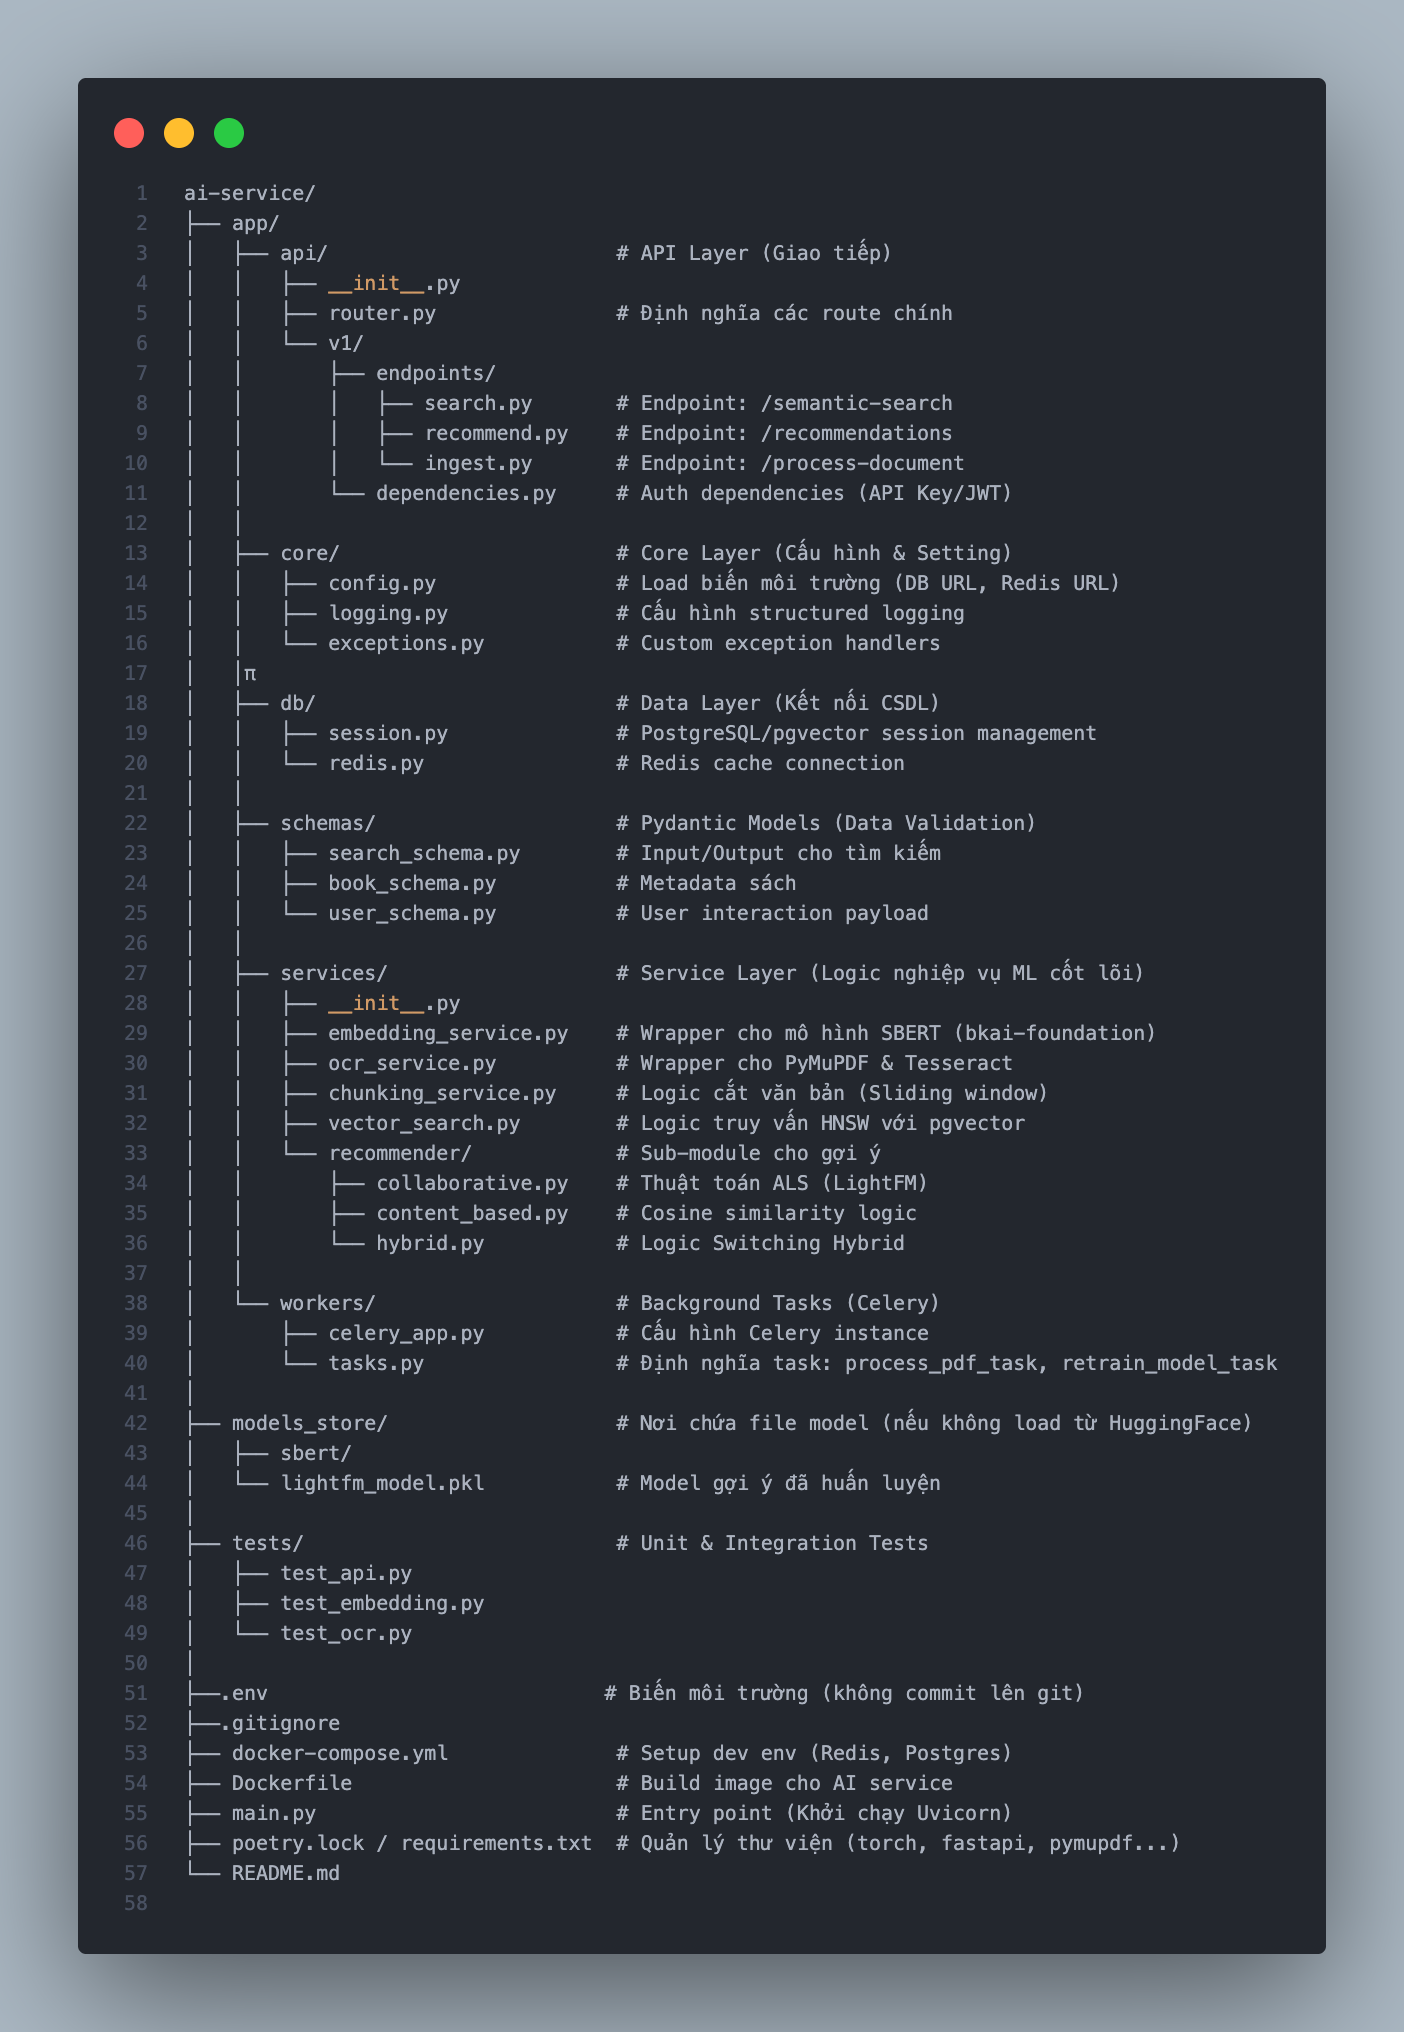
\includegraphics[width=0.95\linewidth]{figures/ch05/architecture/ai_service_architecture.png}
\caption{Kiến trúc chi tiết AI Service và Luồng dữ liệu}
\label{fig:ai_service_architecture_detail}
\end{figure}


%-----------------------------AI-----------------------------------


\subsubsection{Luồng giao tiếp (Communication Flows) nâng cao}

Hệ thống sử dụng hai pattern giao tiếp chính: \textbf{Synchronous Communication} (REST API) cho các tương tác cần phản hồi ngay, và \textbf{Asynchronous Communication} cho các tác vụ không nên chặn luồng nghiệp vụ chính. Ở mức thiết kế, giao tiếp bất đồng bộ được tách thành ba nhóm: Kafka/WebSocket cho notification nội bộ, scheduler/executor cho tác vụ định kỳ hoặc nền trong backend, và queue/callback cho pipeline AI xử lý tài liệu.

\textbf{1. Giao tiếp đồng bộ (Synchronous Communication - REST API):}

Được sử dụng khi:
\begin{itemize}
    \item Frontend cần phản hồi ngay lập tức để hiển thị cho người dùng.
    \item Thao tác đọc dữ liệu (queries) không có side effects.
    \item Validation errors cần trả về trực tiếp cho người dùng.
    \item Cần đảm bảo transaction hoàn thành trước khi tiếp tục workflow.
\end{itemize}

\textbf{Ví dụ 1: Semantic Search Flow}
Luồng tìm kiếm ngữ nghĩa yêu cầu phản hồi nhanh để UX tốt:

\begin{enumerate}
    \item User nhập query "sách về machine learning" trên giao diện tìm kiếm.

    \item \texttt{React/Vite Frontend} gửi \texttt{POST /api/v1/ai/semantic-search} đến Backend Monolith với payload JSON chứa query string và limit.

   \item \texttt{Backend} (\texttt{AiSearchController}/\texttt{AiGatewayService}) xử lý:
    \begin{itemize}
        \item Validate JWT token và extract user info.
        \item Validate query và giới hạn số lượng kết quả.
        \item Chuyển tiếp query sang AI Service qua \texttt{AiGatewayService}; lịch sử tìm kiếm được ghi nhận ở luồng frontend/backend riêng khi người dùng thực hiện tìm kiếm.
        \item Forward request đến AI Service qua internal network.
    \end{itemize}

    \item \texttt{Backend} gọi \texttt{POST http://ai-service:8000/api/v1/semantic-search}
    (internal URL, không expose ra internet).

    \item \texttt{AI Service} xử lý:
    \begin{itemize}
        \item Embedding Service chuyển query thành vector 768 chiều.
        \item Vector Search Service thực hiện ANN search trên bảng vector chunk bằng pgvector.
        \item Gom các chunk gần nhất về danh sách publication IDs với similarity scores.
    \end{itemize}

    \item \texttt{Backend} nhận response từ AI Service:
    \begin{itemize}
        \item Kiểm tra lỗi/timeout từ AI service và fallback sang tìm kiếm catalog nếu cần.
        \item Log request (userId, query, resultCount, responseTime) để phân tích.
    \end{itemize}

    \item \texttt{Backend} query PostgreSQL để lấy metadata chi tiết
    (title, author, cover, availability) của các publication IDs.

    \item \texttt{Backend} merge AI results + metadata, trả về Frontend.

    \item Frontend render kết quả tìm kiếm.
\end{enumerate}

\textbf{Đặc điểm kỹ thuật:}
\begin{itemize}
    \item \textbf{Request-Response pattern:} Client chờ response trước khi tiếp tục (blocking call).
    \item \textbf{Timeout handling:} Backend cấu hình timeout khi gọi AI service để tránh làm treo request người dùng.
    \item \textbf{Fallback:} Nếu AI service lỗi, hệ thống vẫn có thể trả kết quả từ tìm kiếm keyword/catalog truyền thống.
    \item \textbf{Tách trách nhiệm:} AI service chỉ trả về ranking theo ngữ nghĩa; backend chịu trách nhiệm lấy metadata, tình trạng bản sao và quyền truy cập.
\end{itemize}

\textbf{2. Giao tiếp bất đồng bộ - Sự kiện nội bộ và Kafka/WebSocket:}

Backend sử dụng các cơ chế bất đồng bộ cho những tác vụ không nên làm chậm request chính, đặc biệt là gửi email, tạo thông báo, đẩy realtime và xử lý tác vụ nền.

\textbf{Đặc điểm:}
\begin{itemize}
    \item Kafka được dùng để tách các tác vụ notification/email khỏi transaction nghiệp vụ chính.
    \item WebSocket/STOMP được dùng để đẩy thông báo realtime đến frontend sau khi thông báo được tạo.
    \item Các tác vụ nền được xử lý bằng executor/scheduler khi cần, ví dụ kiểm tra trạng thái quá hạn hoặc hết hạn nhận sách theo lịch.
\end{itemize}
\textbf{Ví dụ 2: Quy trình Trả sách và Tính toán Phạt (Return Book with Fine Calculation)}

Khi người dùng trả sách, hàng loạt các tác vụ phụ (side effects) cần được thực hiện. Tuy nhiên, để đảm bảo trải nghiệm người dùng, các tác vụ này không được phép làm chặn (block) phản hồi của API chính:

\begin{enumerate}
    \item Thủ thư thực hiện trả sách thông qua API \texttt{POST /api/v1/transactions/return}.

    \item \texttt{ReturnBookUseCase} bên trong \textbf{Mô-đun Circulation} thực hiện:
    \begin{itemize}
        \item Tải \texttt{BorrowingTransaction} đang hoạt động từ cơ sở dữ liệu.
        \item Kiểm tra bản sao tương ứng với barcode hoặc item id.
        \item Cập nhật ngày trả và trạng thái giao dịch thành đã trả.
        \item Tính toán trễ hạn dựa trên \texttt{dueDate}; nếu quá hạn, tạo bản ghi phí phạt.
        \item Cập nhật trạng thái bản sao về khả dụng hoặc trạng thái phù hợp nếu có sự cố.
        \item Gửi thông báo/email cho bạn đọc thông qua hạ tầng notification.
    \end{itemize}

    \item Giao dịch cơ sở dữ liệu hoàn tất, API trả kết quả cho thủ thư gồm trạng thái trả sách, ngày trả, số ngày quá hạn và phí phát sinh nếu có.

    \item Các tác vụ phụ như gửi thông báo, email hoặc cập nhật dashboard được xử lý sau luồng chính để thao tác trả sách tại quầy không bị chậm.
\end{enumerate}

\textbf{Lợi ích của Internal Events:}
\begin{itemize}
    \item \textbf{Decoupling:} Circulation Module không phải tự xử lý mọi side effect như email, notification realtime hay thống kê.
    \item \textbf{Single Responsibility:} Mỗi module chỉ quan tâm đến domain logic của mình.
    \item \textbf{Extensibility:} Có thể bổ sung loại thông báo mới hoặc kênh gửi mới mà không phải viết lại nghiệp vụ trả sách.
    \item \textbf{Transaction safety:} Trạng thái giao dịch, bản sao và phí phạt được cập nhật trong luồng nghiệp vụ chính trước khi phát sinh side effect.
    \item \textbf{Testability:} Có thể kiểm thử use case trả sách độc lập với kênh gửi thông báo.
\end{itemize}

\textbf{3. Giao tiếp bất đồng bộ với AI Service:}

Với xử lý PDF, hệ thống không để request upload phải chờ toàn bộ pipeline AI hoàn tất. Backend lưu thông tin tài liệu, ghi trạng thái ETL và kích hoạt AI service bằng REST trong một tác vụ nền. AI service có thể xử lý trực tiếp qua FastAPI hoặc qua worker nền khi cần mở rộng, nhưng hợp đồng chính giữa backend và AI vẫn là API rõ ràng.

\textbf{Đặc điểm kỹ thuật:}
\begin{itemize}
    \item \textbf{Không chặn luồng nghiệp vụ:} Thủ thư có thể hoàn tất thao tác tạo/cập nhật ấn phẩm trước khi AI xử lý xong PDF.
    \item \textbf{Theo dõi trạng thái:} Backend lưu trạng thái \texttt{QUEUED}, \texttt{SUCCESS} hoặc \texttt{FAILED} trong bảng ETL để giao diện có thể hiển thị tiến độ.
    \item \textbf{Fallback:} Nếu AI hoặc Gemini lỗi, ấn phẩm vẫn tồn tại trong catalog và hệ thống vẫn hỗ trợ tìm kiếm keyword.
    \item \textbf{Callback có xác thực:} Backend có endpoint callback được bảo vệ bằng chữ ký HMAC để nhận kết quả từ AI worker khi chạy theo kiểu worker/callback.
\end{itemize}

\textbf{Ví dụ 3: Quy trình Thêm sách mới kèm Xử lý PDF (Add Book with PDF Processing)}

Quá trình xử lý PDF, sinh embedding và gọi Gemini có thể tốn thời gian, do đó không nên sử dụng cơ chế chặn (blocking) trên request của thủ thư:

\begin{enumerate}
    \item Thủ thư tạo ấn phẩm mới thông qua API \texttt{POST /api/v1/publications} với metadata như tiêu đề, ISBN, tác giả, nhà xuất bản, danh mục, tag, ngôn ngữ và năm xuất bản.

    \item \texttt{CreatePublicationUseCase} và các use case upload tài liệu trong \textbf{Mô-đun Danh mục (Catalog Module)} thực hiện:
    \begin{itemize}
        \item Kiểm tra hợp lệ metadata và các quan hệ với tác giả, nhà xuất bản, danh mục, tag.
        \item Tạo đối tượng \texttt{Publication}.
        \item Upload ảnh bìa nếu có thông qua endpoint cover.
        \item Cấp presigned URL để frontend upload PDF lên S3-compatible storage.
        \item Lưu dữ liệu vào PostgreSQL.
        \item Khi frontend gửi document URL về backend, hệ thống ghi trạng thái ETL \texttt{QUEUED} và gọi AI service xử lý tài liệu.
    \end{itemize}

    \item API trả về mã HTTP 201 Created hoặc kết quả cập nhật document URL ngay sau khi metadata/PDF URL được lưu, không chờ toàn bộ AI pipeline.

    \item Thủ thư nhận trạng thái "đang xử lý AI" và có thể tiếp tục thực hiện công việc khác.

    \item \textbf{Dịch vụ AI} nhận yêu cầu xử lý \texttt{POST /api/v1/publications/process}:
    \begin{itemize}
        \item Nhận \texttt{publicationId}, \texttt{pdfUrl} và cờ \texttt{forceReprocess}.
        \item Tải PDF từ S3-compatible storage.
        \item Trích xuất văn bản bằng PyMuPDF và làm sạch header/footer, số trang, ký tự lỗi.
        \item Chia văn bản thành các chunk 1500 ký tự, overlap 150 ký tự.
        \item Tạo embedding 768 chiều cho từng chunk và lưu vào \texttt{ai\_engine.publication\_vectors}.
        \item Chọn các chunk đại diện, gọi Gemini để tạo summary, audience và tag; nếu lỗi thì dùng fallback deterministic.
        \item Cập nhật metadata AI và trạng thái ETL trong PostgreSQL.
    \end{itemize}

    \item Sau khi hoàn tất (hoặc thất bại sau tất cả lần thử):
    \begin{itemize}
        \item AI service trả kết quả cho backend hoặc cập nhật qua callback \texttt{POST /api/ai/callback} khi chạy theo mô hình worker.
        \item Backend cập nhật trạng thái xử lý AI.
        \item Nếu cần, hệ thống gửi thông báo cho thủ thư về kết quả xử lý.
    \end{itemize}

    \item Kết quả: Nếu xử lý thành công, sách xuất hiện trong kết quả tìm kiếm ngữ nghĩa. Nếu thất bại, sách vẫn có trong danh mục nhưng chỉ hỗ trợ tìm kiếm theo từ khóa truyền thống.
\end{enumerate}

\textbf{Đặc điểm của mẫu xử lý nền cho AI:}
\begin{itemize}
    \item \textbf{Xử lý bất đồng bộ (Async processing):} Backend không bị chặn (non-blocking), trả phản hồi ngay lập tức cho người dùng để tối ưu trải nghiệm.
    \item \textbf{Idempotent processing:} AI pipeline dùng \texttt{publicationId}, hash file và cờ \texttt{forceReprocess} để tránh xử lý trùng không cần thiết.
    \item \textbf{Khả năng phục hồi:} Khi PDF lỗi, Gemini rate-limit hoặc AI service tạm thời không phản hồi, hệ thống ghi trạng thái thất bại thay vì làm hỏng dữ liệu catalog.
    \item \textbf{Mở rộng từng bước:} Khi tải tăng, AI service có thể bổ sung worker/Celery để xử lý hàng đợi nội bộ mà không cần thay đổi nghiệp vụ frontend/backend.
    \item \textbf{Tách rủi ro AI khỏi nghiệp vụ chính:} Tạo sách, quản lý bản sao, mượn--trả và thanh toán không phụ thuộc tuyệt đối vào kết quả AI.
\end{itemize}

\textbf{4. Chuỗi sự kiện lan truyền - Quy trình nghiệp vụ đa mô-đun phức tạp (Event Cascade)}

Một số quy trình công việc (workflows) đòi hỏi sự kết hợp giữa cả gọi đồng bộ (sync calls) và sự kiện bất đồng bộ (async events) để đạt được sự cân bằng tối ưu giữa tính nhất quán dữ liệu (consistency) và hiệu năng (performance).

\textbf{Ví dụ 4: Quy trình Mượn sách hoàn chỉnh (Borrow Book - Complete Workflow)}

\begin{enumerate}
    \item \textbf{Giai đoạn 1: Kiểm tra hợp lệ Đồng bộ (Synchronous Validation)}
    \begin{itemize}
        \item Bạn đọc nhấn "Mượn sách" $\rightarrow$ Frontend gửi yêu cầu \texttt{POST /api/v1/transactions/borrow}; nếu thủ thư cho mượn tại quầy, frontend dùng \texttt{POST /api/v1/transactions/borrow-direct}.
        \item \texttt{BorrowingTransactionController} kiểm tra JWT, vai trò và tính hợp lệ của request.
        \item Use case kiểm tra tài khoản người dùng, phí phạt còn tồn tại, số lượng sách đang mượn và tình trạng bản sao/ấn phẩm.
        \item Với yêu cầu từ bạn đọc, hệ thống tạo giao dịch chờ xác nhận nhận sách. Với mượn trực tiếp, hệ thống ghi nhận bản sao cụ thể và ngày đến hạn.
        \item Tạo \texttt{BorrowingTransaction}, lưu vào cơ sở dữ liệu, cập nhật trạng thái bản sao khi cần và cam kết giao dịch.
        \item API trả về mã \texttt{201 Created} (tổng thời gian: $\sim$200ms).
    \end{itemize}

    \item \textbf{Giai đoạn 2: Tác vụ phụ sau giao dịch}
    \begin{itemize}
        \item Hệ thống tạo thông báo cho bạn đọc và/hoặc thủ thư tùy theo trạng thái giao dịch.
        \item Kafka/WebSocket giúp đẩy thông báo mà không làm chậm API chính.
        \item Mô-đun recommendation ghi nhận tương tác mượn để phục vụ mô hình gợi ý.
        \item Dashboard thủ thư phản ánh số lượng giao dịch mới, sách đang mượn và các yêu cầu cần xử lý.
    \end{itemize}

    \item \textbf{Giai đoạn 3: Tác động đến AI Recommendation}
    \begin{itemize}
        \item Dữ liệu tương tác mới được lưu trong PostgreSQL.
        \item Khi người dùng gọi API gợi ý, backend gọi AI service \texttt{POST /api/v1/recommendations}.
        \item AI service dùng ALS đã train, content-based và trending fallback để trả danh sách mới; mô hình ALS được refresh theo lịch hoặc khi gọi endpoint refresh.
    \end{itemize}
\end{enumerate}

\textbf{Dòng thời gian xử lý (Timeline):}
\begin{itemize}
    \item \textbf{T+0ms:} Người dùng nhấn nút "Mượn sách".
    \item \textbf{T+200ms:} API phản hồi \texttt{201 Created} $\rightarrow$ Người dùng thấy thông báo "Mượn sách thành công".
    \item \textbf{T+300ms:} Thông báo và các tác vụ phụ được xử lý nền.
    \item \textbf{T+vài giây/phút:} Dữ liệu tương tác được AI service sử dụng trong lần suy luận hoặc refresh recommendation tiếp theo.
\end{itemize}

\textbf{Lợi ích kiến trúc:}
\begin{itemize}
    \item \textbf{Phản hồi nhanh (Fast response):} Người dùng không phải chờ AI xử lý xong mới mượn được sách.
    \item \textbf{Tính nhất quán mạnh (Strong consistency):} Giao dịch cốt lõi (bản ghi mượn sách, kho hàng) đảm bảo nhất quán tuyệt đối nhờ ACID transaction.
    \item \textbf{Tính nhất quán cuối cùng (Eventual consistency):} Dữ liệu gợi ý có thể cập nhật sau nghiệp vụ mượn sách; đây là độ trễ chấp nhận được vì recommendation không quyết định tính đúng sai của giao dịch.
    \item \textbf{Khả năng phục hồi (Resilience):} Nếu Dịch vụ AI gặp sự cố, chức năng mượn sách cốt lõi vẫn hoạt động bình thường, hệ thống chỉ tạm thời dùng gợi ý fallback hoặc kết quả đã lưu trước đó.
\end{itemize}


\subsection{Thiết kế giao diện}

Toàn bộ giao diện hệ thống được thiết kế trên \textbf{Figma} trước khi hiện thực, đảm bảo sự thống nhất về phong cách (Design System) và luồng tương tác (User Flow) giữa các màn hình. Bản thiết kế đầy đủ có thể xem tại đường dẫn trong Phụ lục~\ref{appendix:resources}.

Hệ thống tuân thủ các nguyên tắc thiết kế cốt lõi: \textbf{tính nhất quán} (màu sắc, typography, hành vi component thống nhất toàn ứng dụng), \textbf{phản hồi trạng thái} (loading skeleton khi AI xử lý, toast notification sau thao tác), \textbf{tối giản} (nội dung trọng tâm là sách và thanh tìm kiếm), và \textbf{responsive} (Tailwind CSS Grid đảm bảo hiển thị tốt trên mọi thiết bị). Các component được xây dựng theo thiết kế Figma, kết hợp Tailwind CSS, lucide-react, sonner và một số thư viện nhỏ như react-select, react-day-picker để giữ giao diện linh hoạt nhưng vẫn nhất quán.

\subsubsection{Giao diện Public (Trang chủ và Tìm kiếm)}

\begin{figure}[htbp]
    \centering
    \begin{subfigure}[t]{0.48\linewidth}
        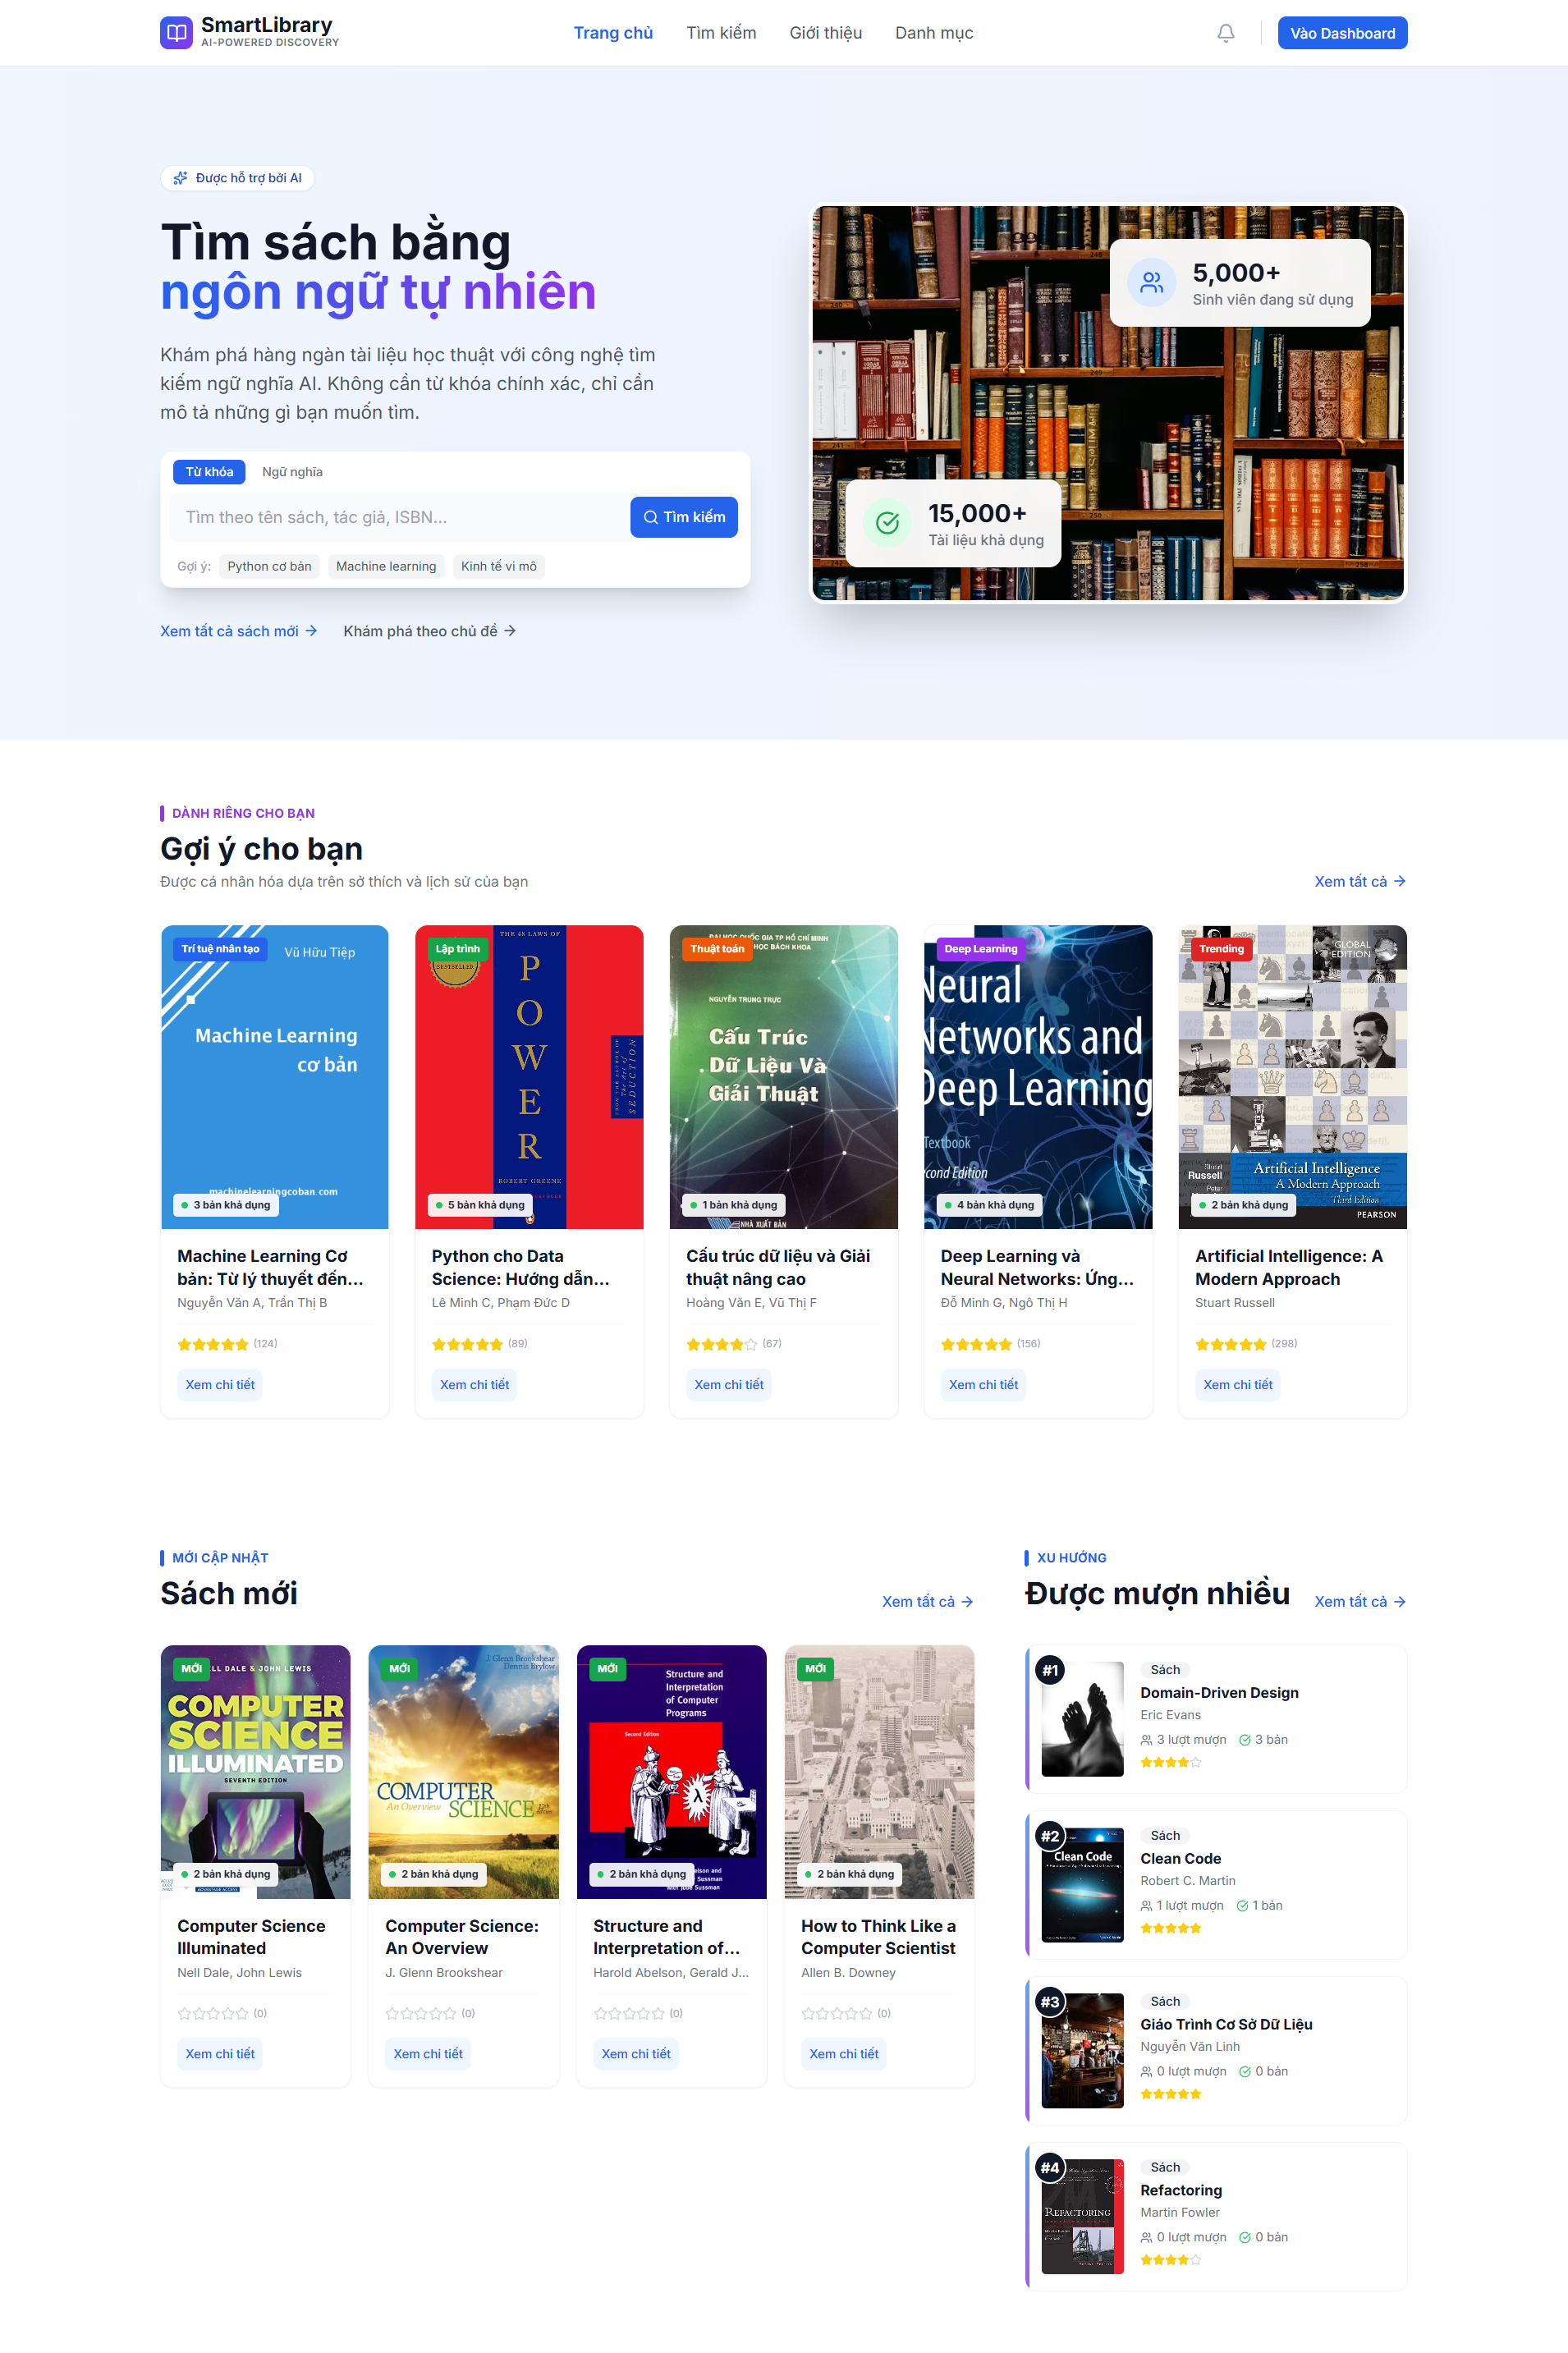
\includegraphics[width=\linewidth, height=0.38\textheight, keepaspectratio]{figures/ch05/ui/public/homepage.png}
        \caption{Trang chủ}
        \label{fig:home_page}
    \end{subfigure}
    \hfill
    \begin{subfigure}[t]{0.48\linewidth}
        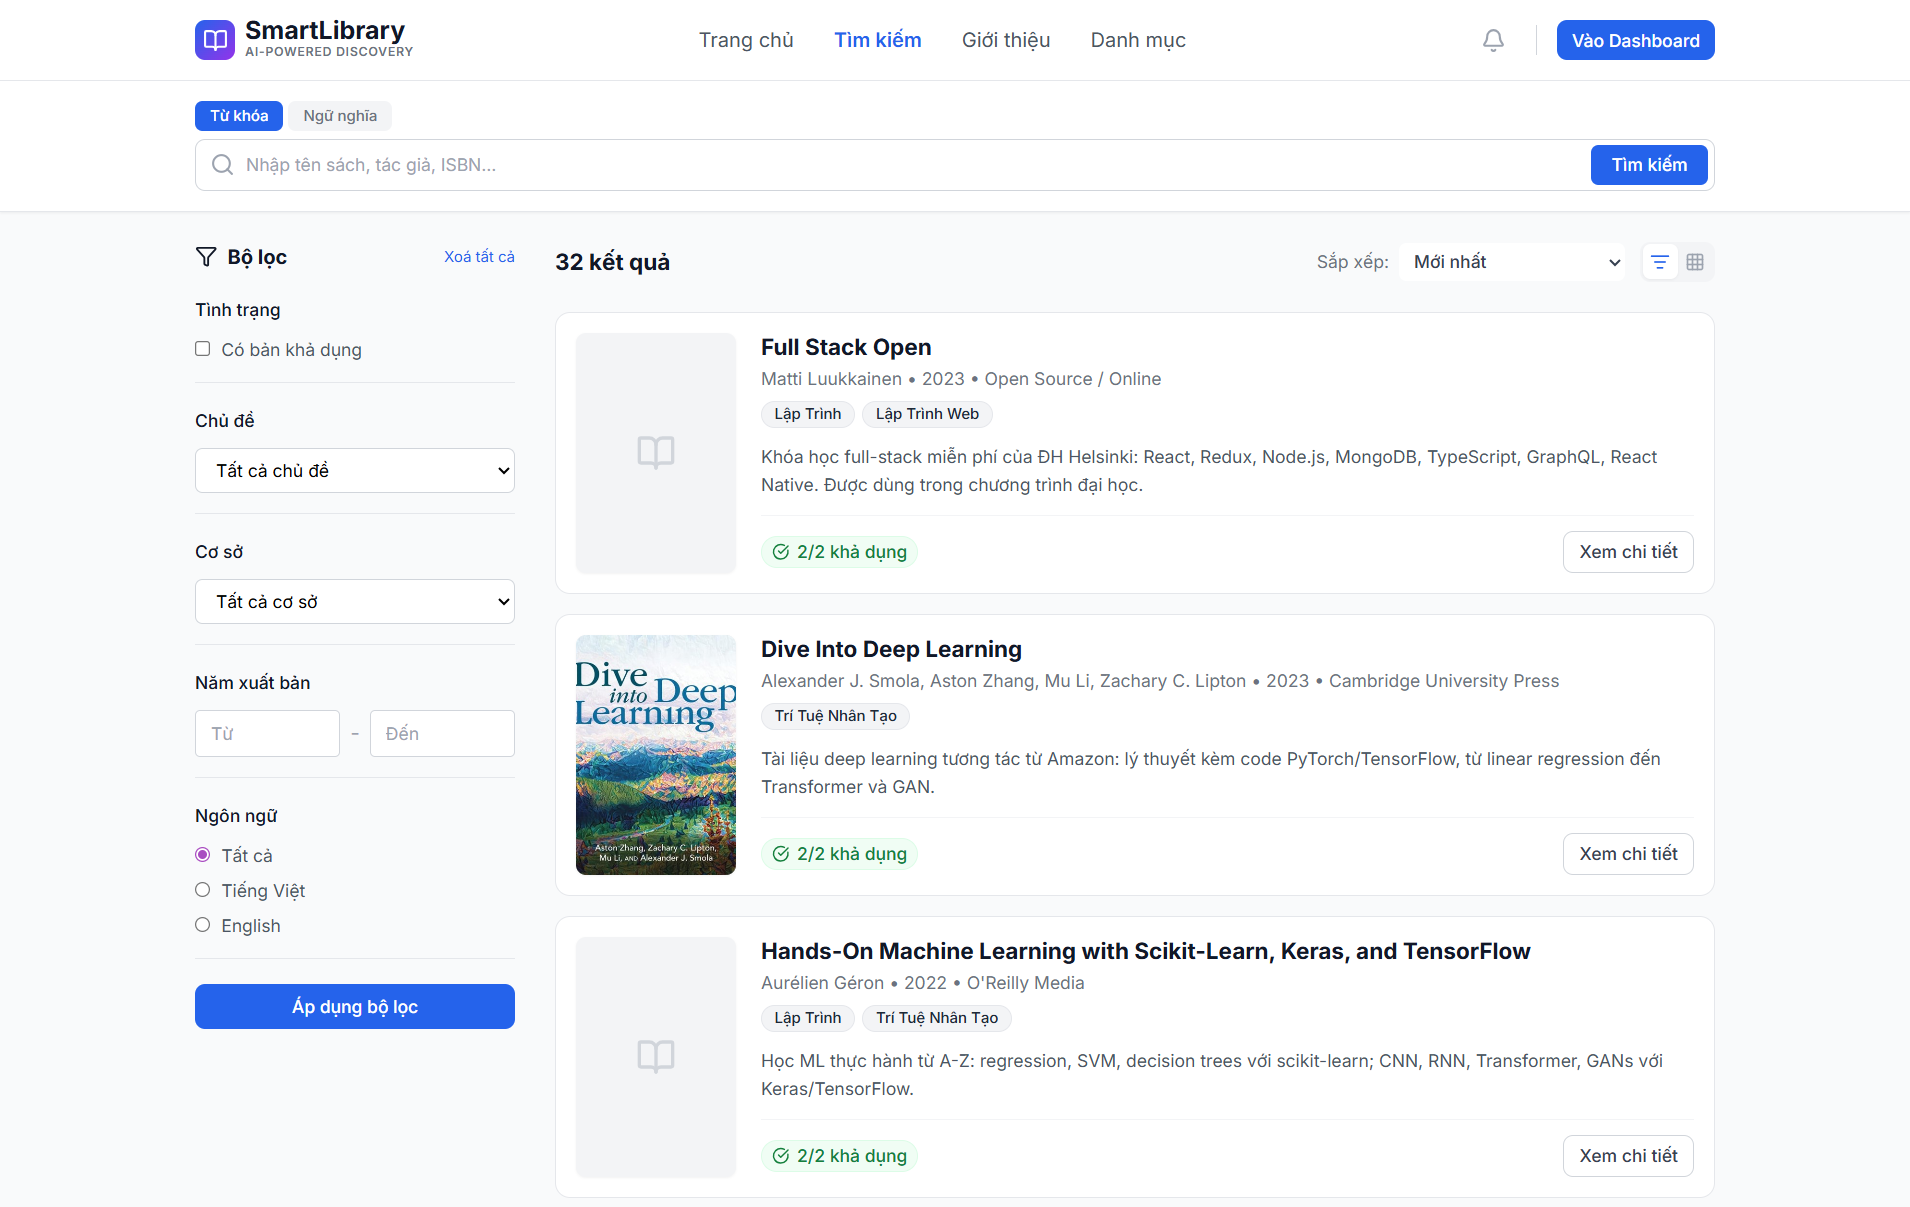
\includegraphics[width=\linewidth, height=0.38\textheight, keepaspectratio]{figures/ch05/ui/public/search_book.png}
        \caption{Tìm kiếm sách với bộ lọc}
        \label{fig:search_book}
    \end{subfigure}
    \caption{Giao diện Public: Trang chủ và Tìm kiếm}
\end{figure}


\begin{figure}[htbp]
    \centering
    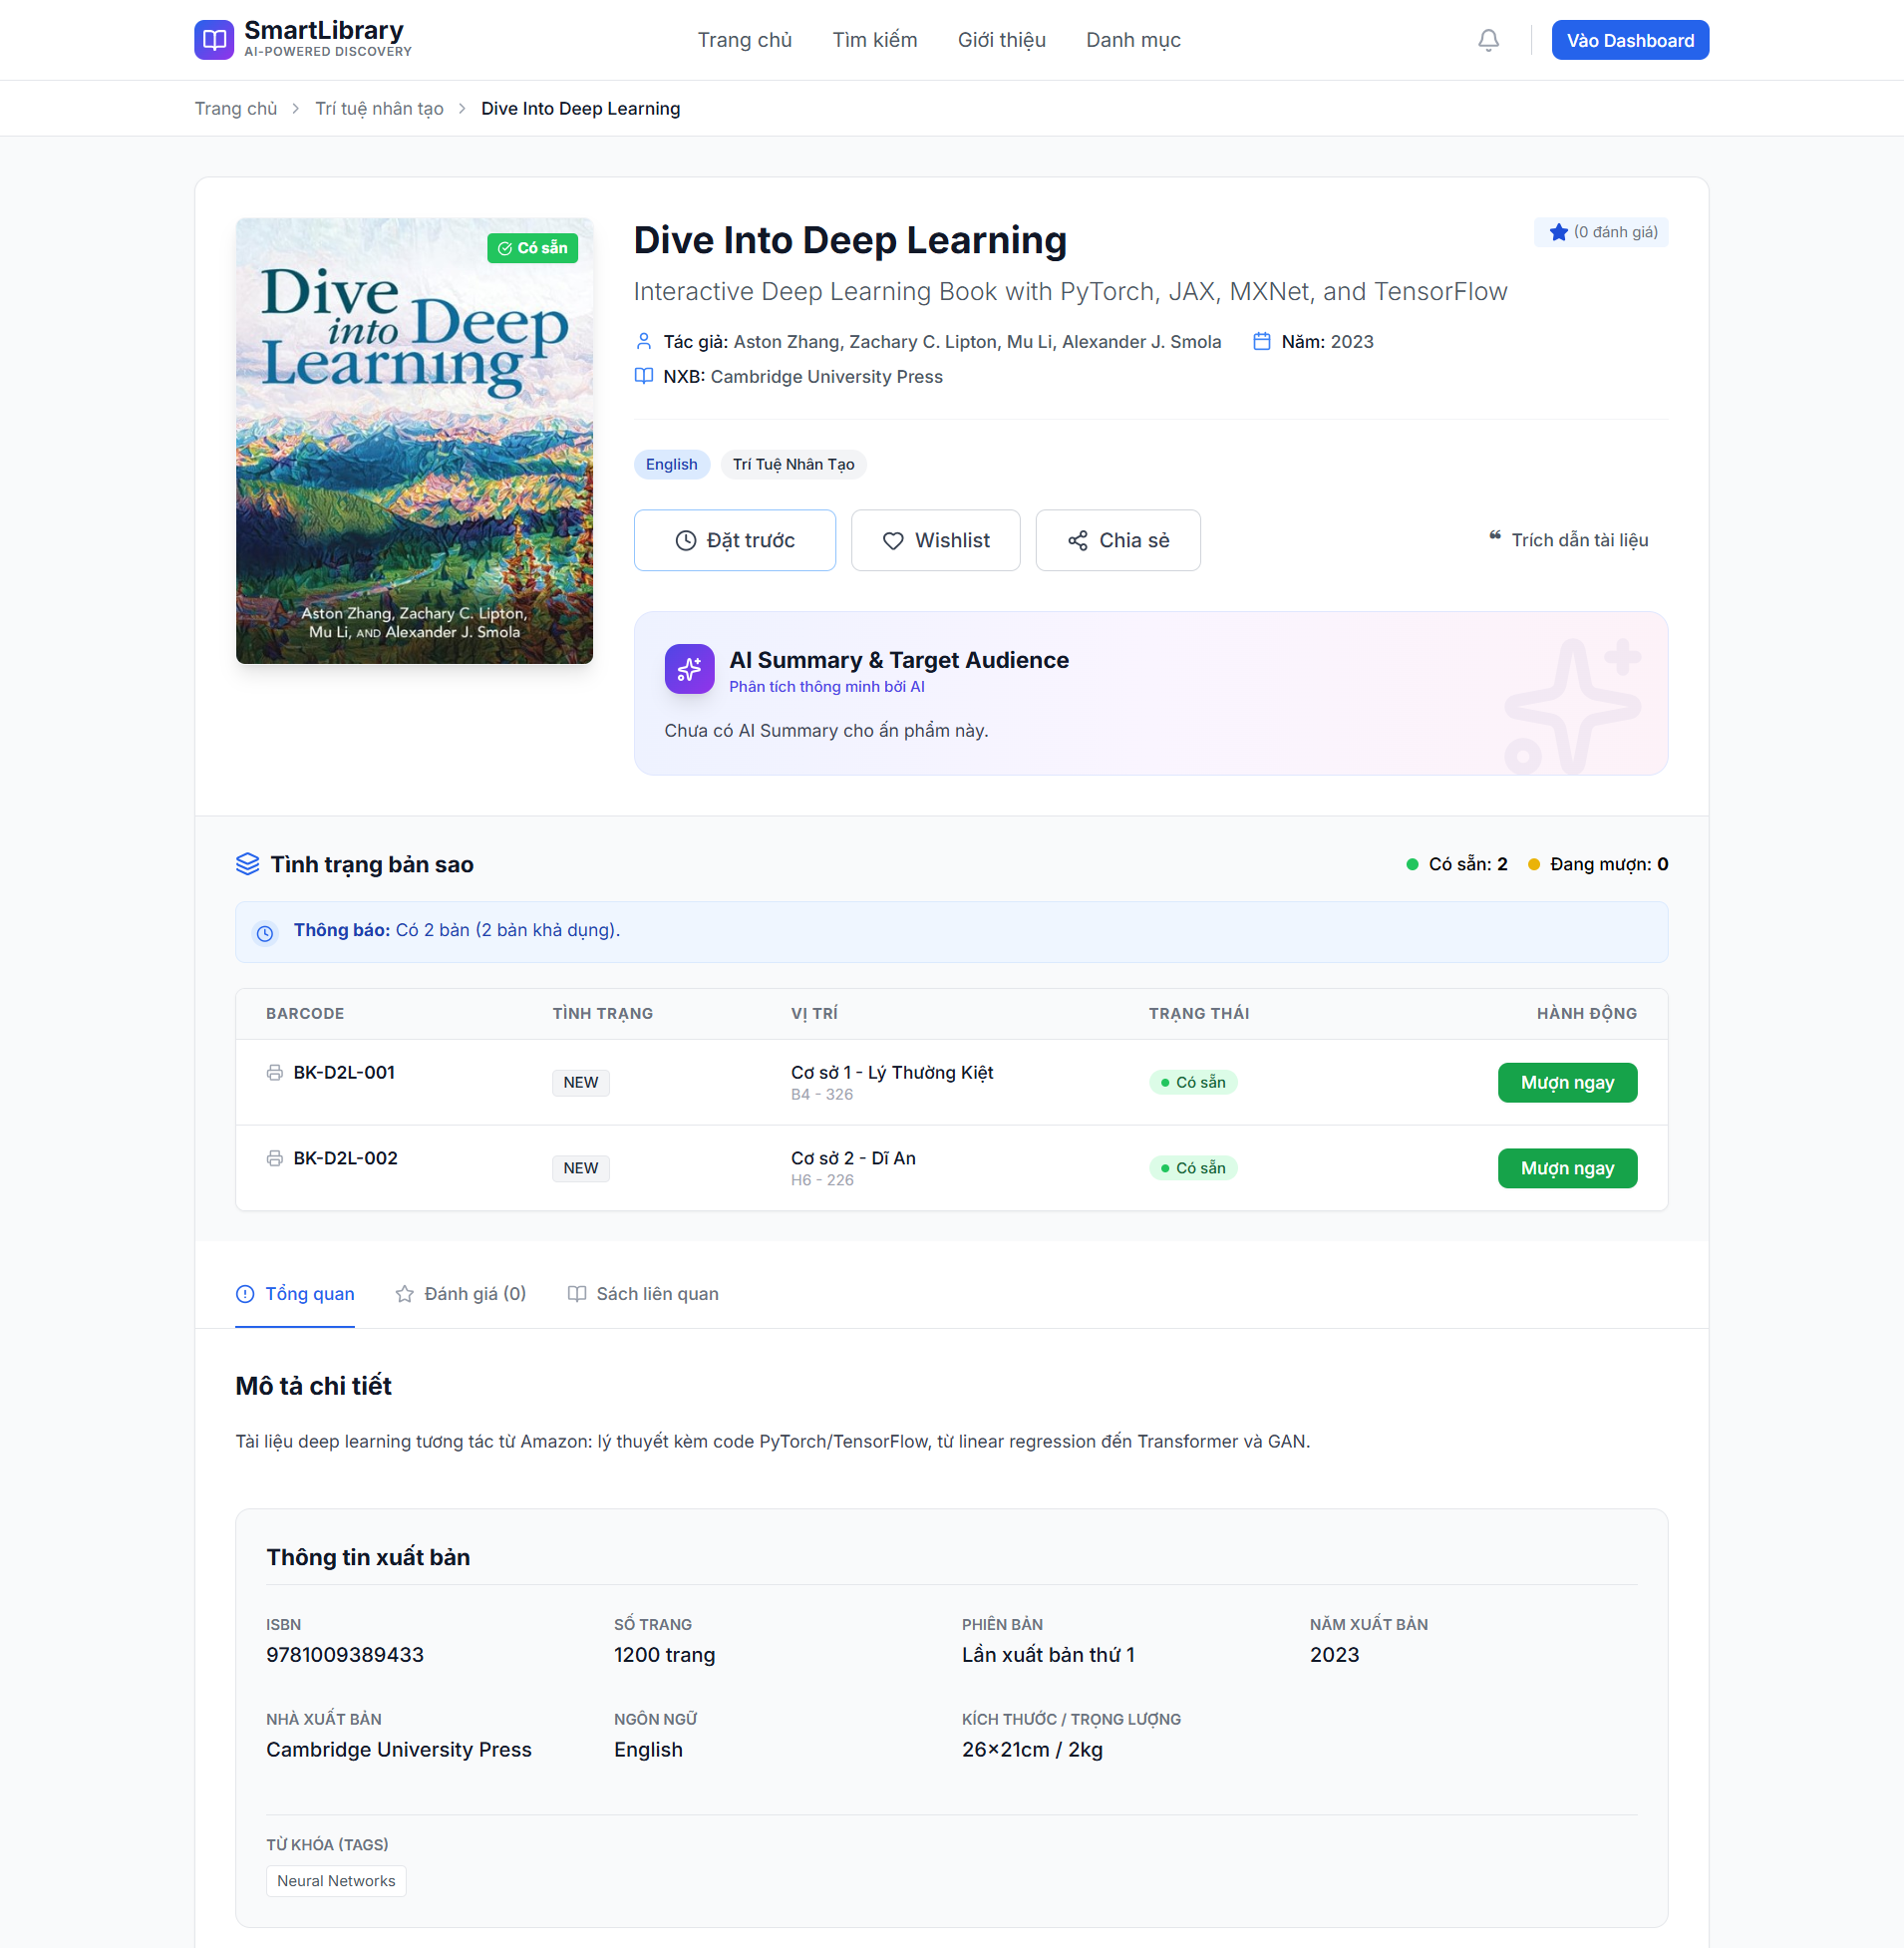
\includegraphics[width=0.6\linewidth]{figures/ch05/ui/public/book_detail.png}
    \caption{Giao diện Chi tiết sách}
    \label{fig:book_detail}
\end{figure}
\FloatBarrier

\subsubsection{Giao diện Độc giả (User Pages)}

\begin{figure}[htbp]
    \centering
    \begin{subfigure}[t]{0.48\linewidth}
        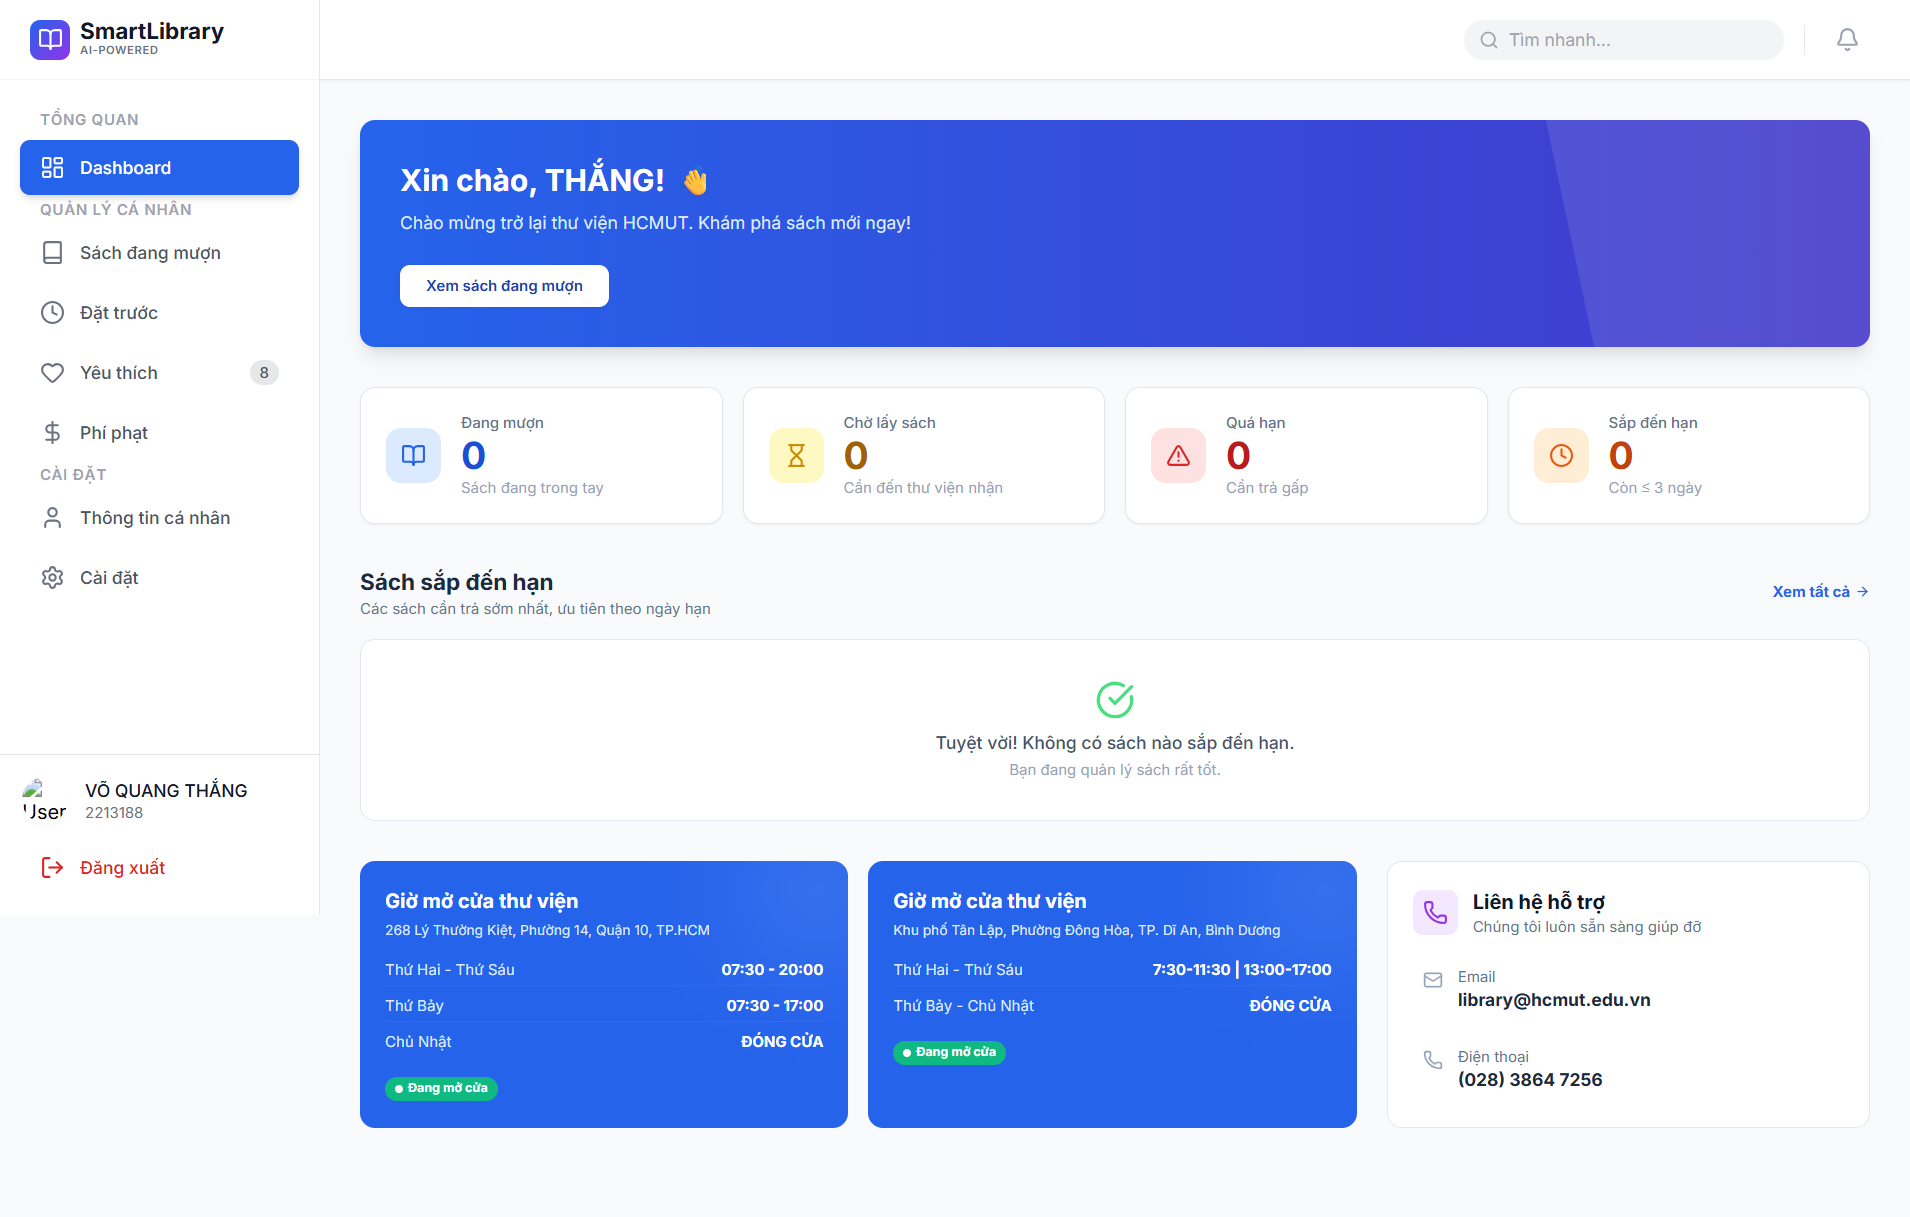
\includegraphics[width=\linewidth, height=0.38\textheight, keepaspectratio]{figures/ch05/ui/reader/dashboard.png}
        \caption{Dashboard tổng quan}
        \label{fig:user_dashboard}
    \end{subfigure}
    \hfill
    \begin{subfigure}[t]{0.48\linewidth}
        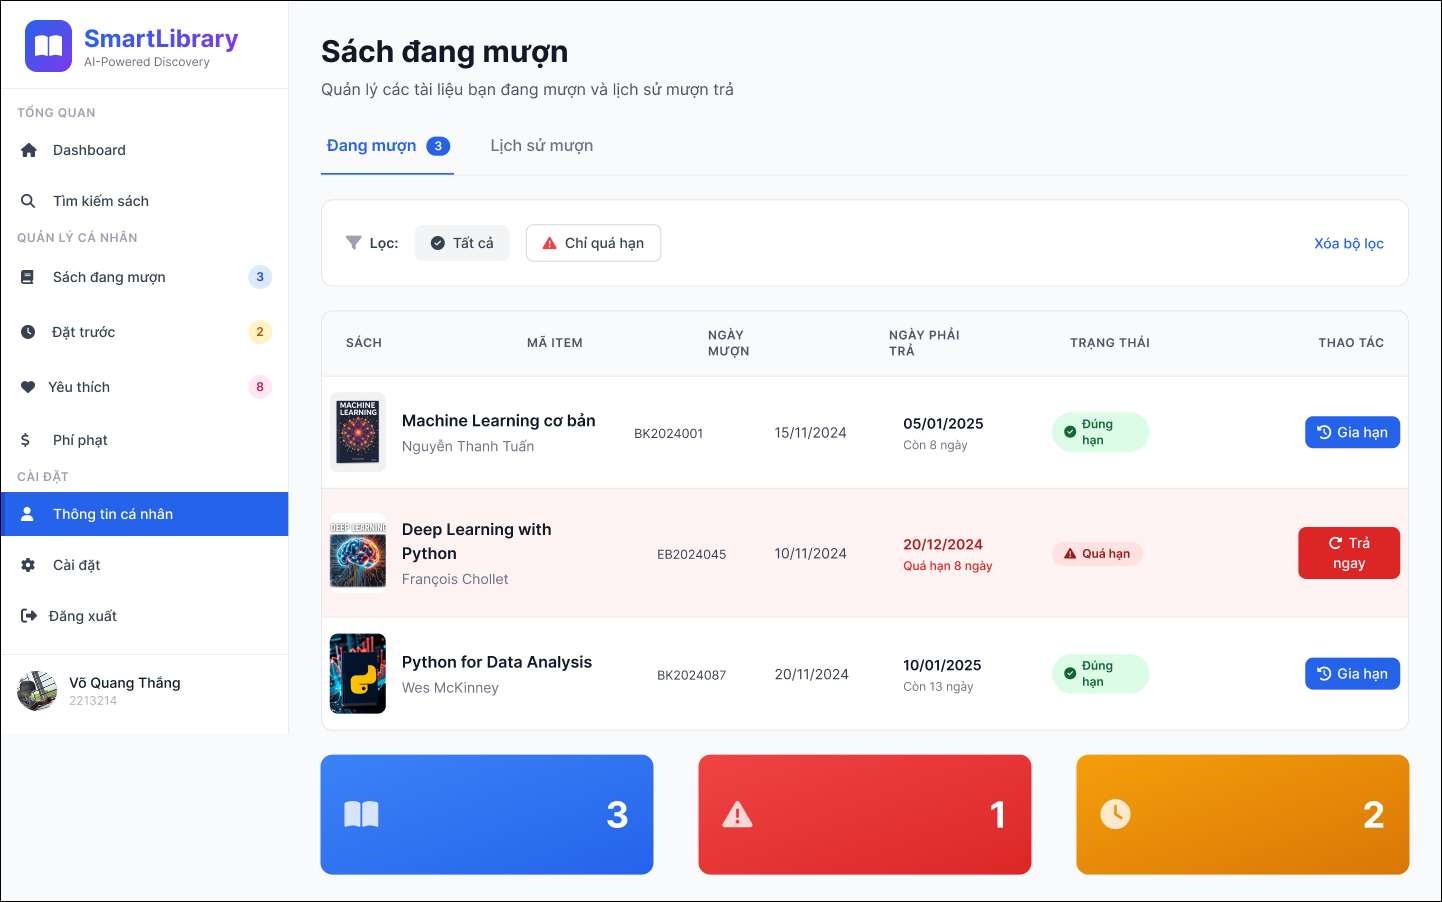
\includegraphics[width=\linewidth, height=0.38\textheight, keepaspectratio]{figures/ch05/ui/reader/current_books.png}
        \caption{Quản lý sách đang mượn}
        \label{fig:user_borrowing}
    \end{subfigure}
    \caption{Giao diện Độc giả: Dashboard và Quản lý mượn sách}
\end{figure}
\FloatBarrier

\subsubsection{Giao diện Thủ thư (Librarian Pages)}

\begin{figure}[htbp]
    \centering
    \begin{subfigure}[t]{0.48\linewidth}
        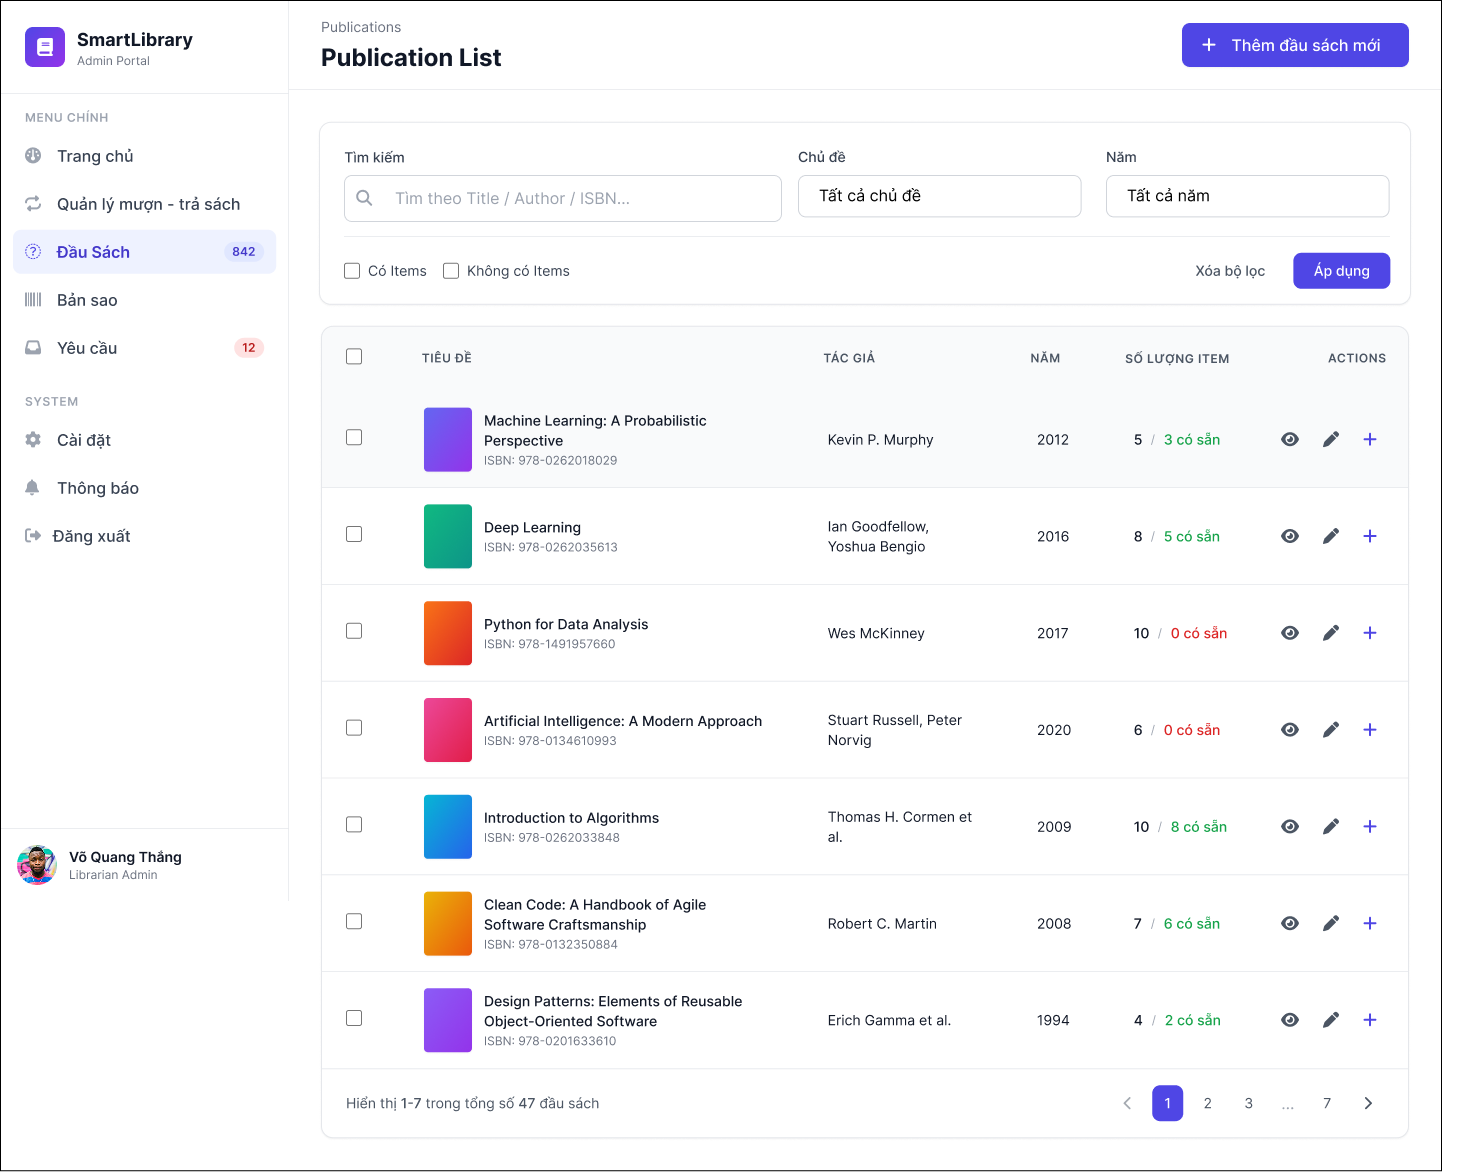
\includegraphics[width=\linewidth, height=0.38\textheight, keepaspectratio]{figures/ch05/ui/librarian/publication_list.png}
        \caption{Quản lý danh mục sách}
        \label{fig:lib_pub_list}
    \end{subfigure}
    \hfill
    \begin{subfigure}[t]{0.48\linewidth}
        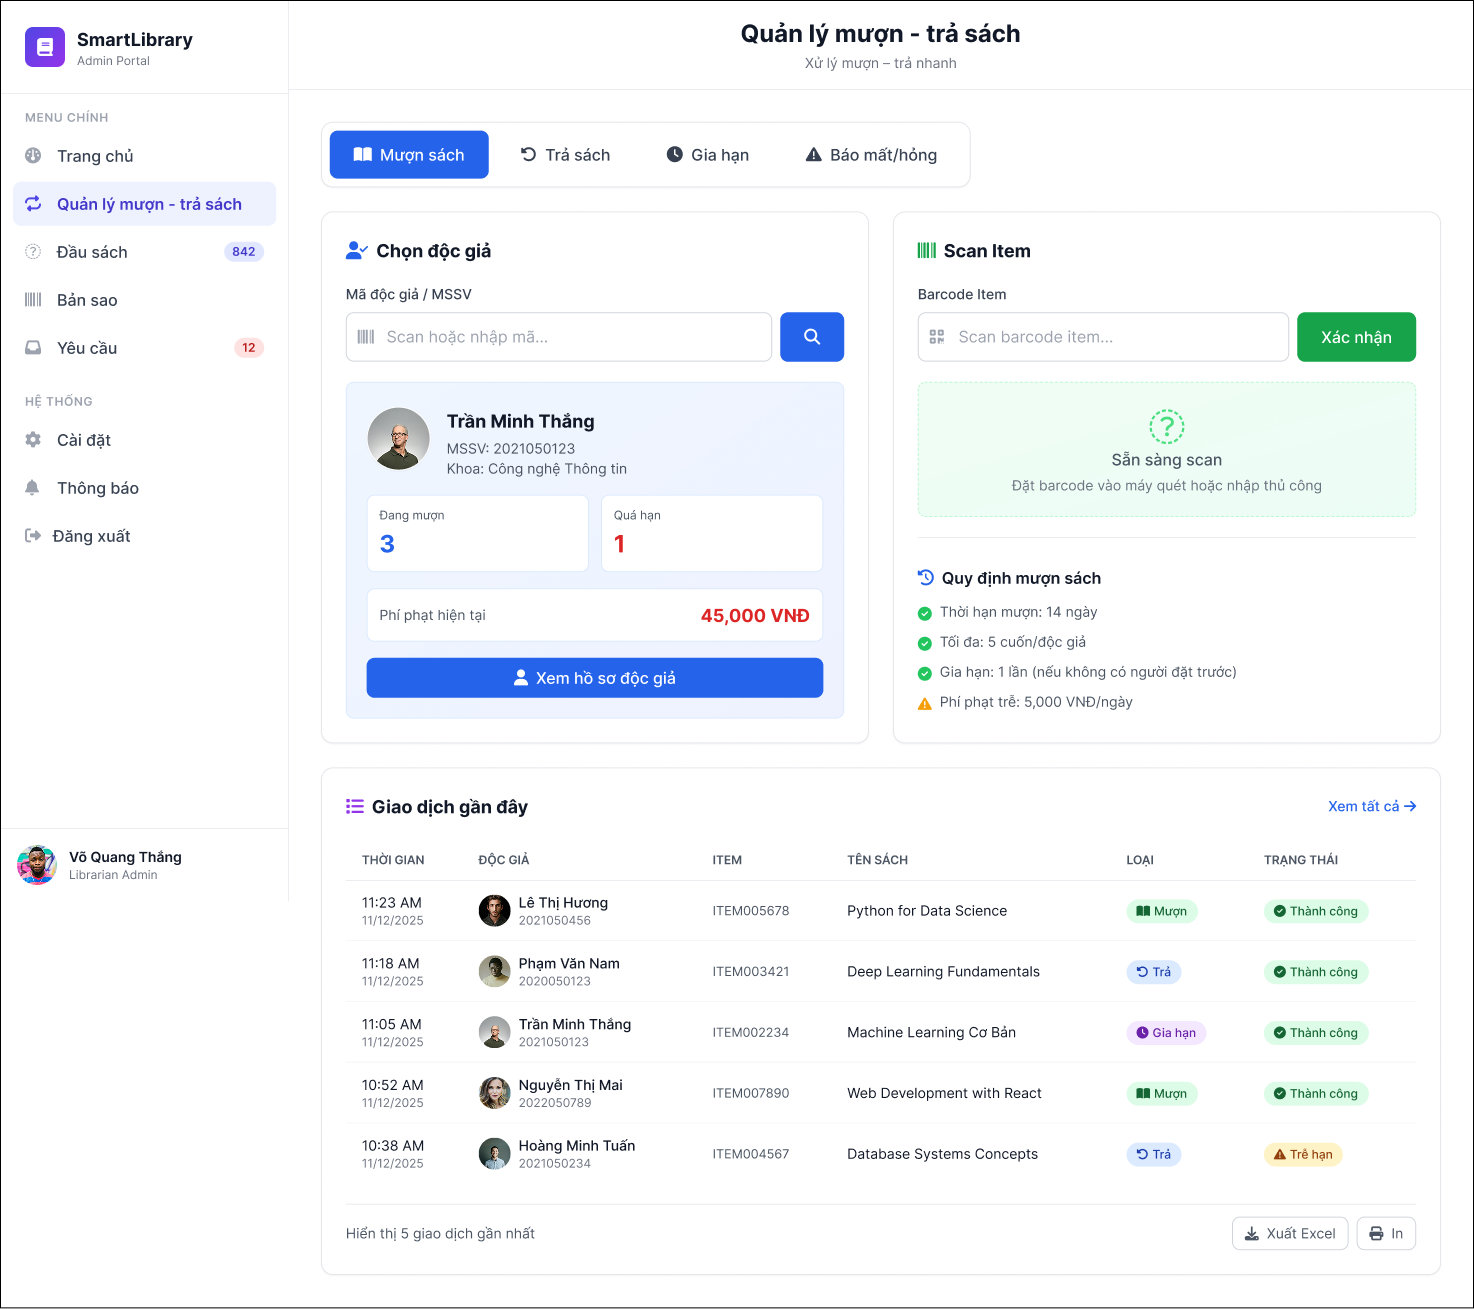
\includegraphics[width=\linewidth, height=0.38\textheight, keepaspectratio]{figures/ch05/ui/librarian/borrow_book.png}
        \caption{Ghi nhận mượn sách (Check-out)}
        \label{fig:lib_checkout}
    \end{subfigure}
    \caption{Giao diện Thủ thư: Quản lý danh mục và Lưu thông}
\end{figure}
\FloatBarrier
